\documentclass[10pt, letterpaper, twoside]{article}
\usepackage[utf8]{inputenc}
\usepackage{geometry}
\usepackage{hyperref}
\usepackage[english]{babel}
 \geometry{
 a4paper,
 total={170mm,257mm},
 left=20mm,
 top=20mm,
 }
\usepackage{graphicx}
\graphicspath{ {./images/} } 
\setcounter{section}{2}
\usepackage[font=small,labelfont=bf]{caption}
 
\title{Assignment 3 \\ MPI Point-to-Point and One-Sided Communication}
\author{Smith Agarwal \\ Shyam Arumugaswamy \\ Siddhesh Kandarkar}
\date{December 20, 2018}
 
\begin{document}
 
\begin{titlepage}
\maketitle


\section{Setting a Baseline}

\subsection{Required submission files}

\begin{enumerate}
\item \textbf{The updated Load-Leveler batch script.} 

Refer job\_updated.ll file from code scripts of Task 3.1   

\item \textbf{The performance plots and description in the report.} 

The various performance plots for the baseline are: \\
\vspace{5mm}
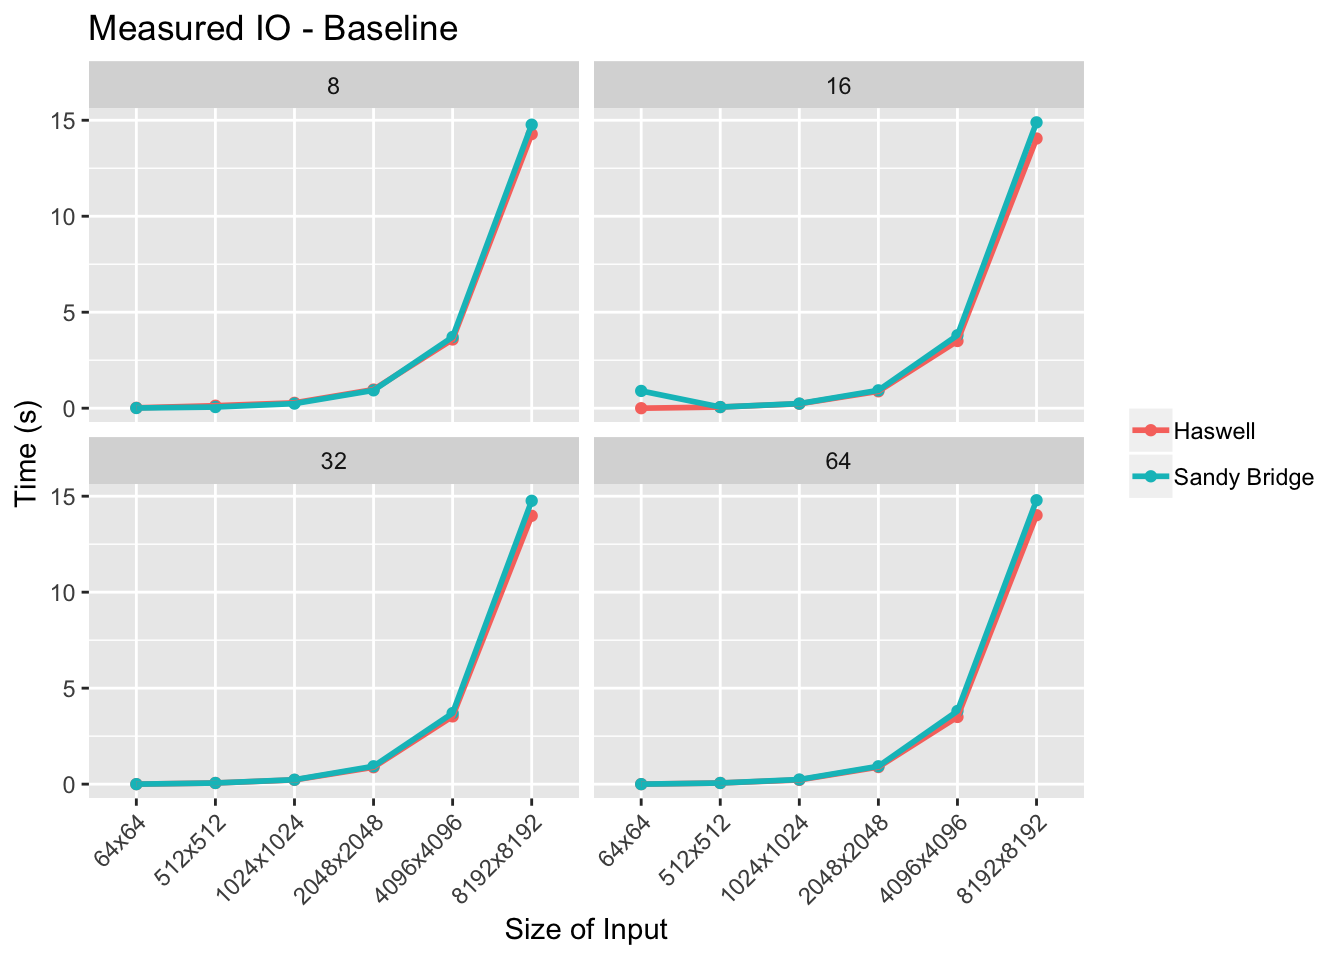
\includegraphics[scale = 0.18]{Baseline_Measured-IO_Processes.png}
%\captionof{figure}{example code for adding pic} 
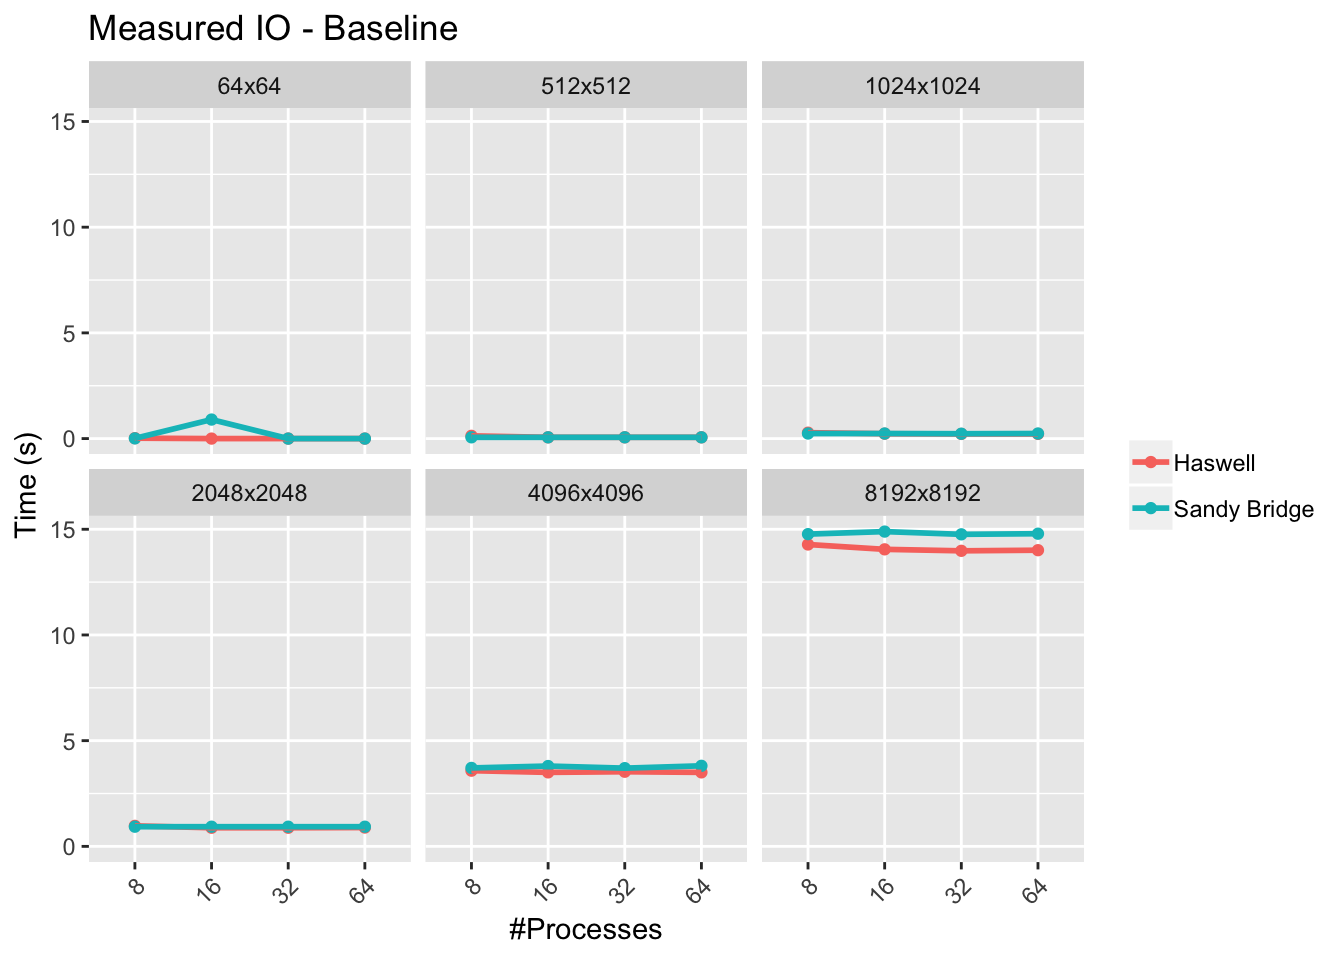
\includegraphics[scale = 0.18]{Baseline_Measured-IO_InputSize.png}
%\captionof{figure}{example code for adding pic} 
\vspace{5mm}
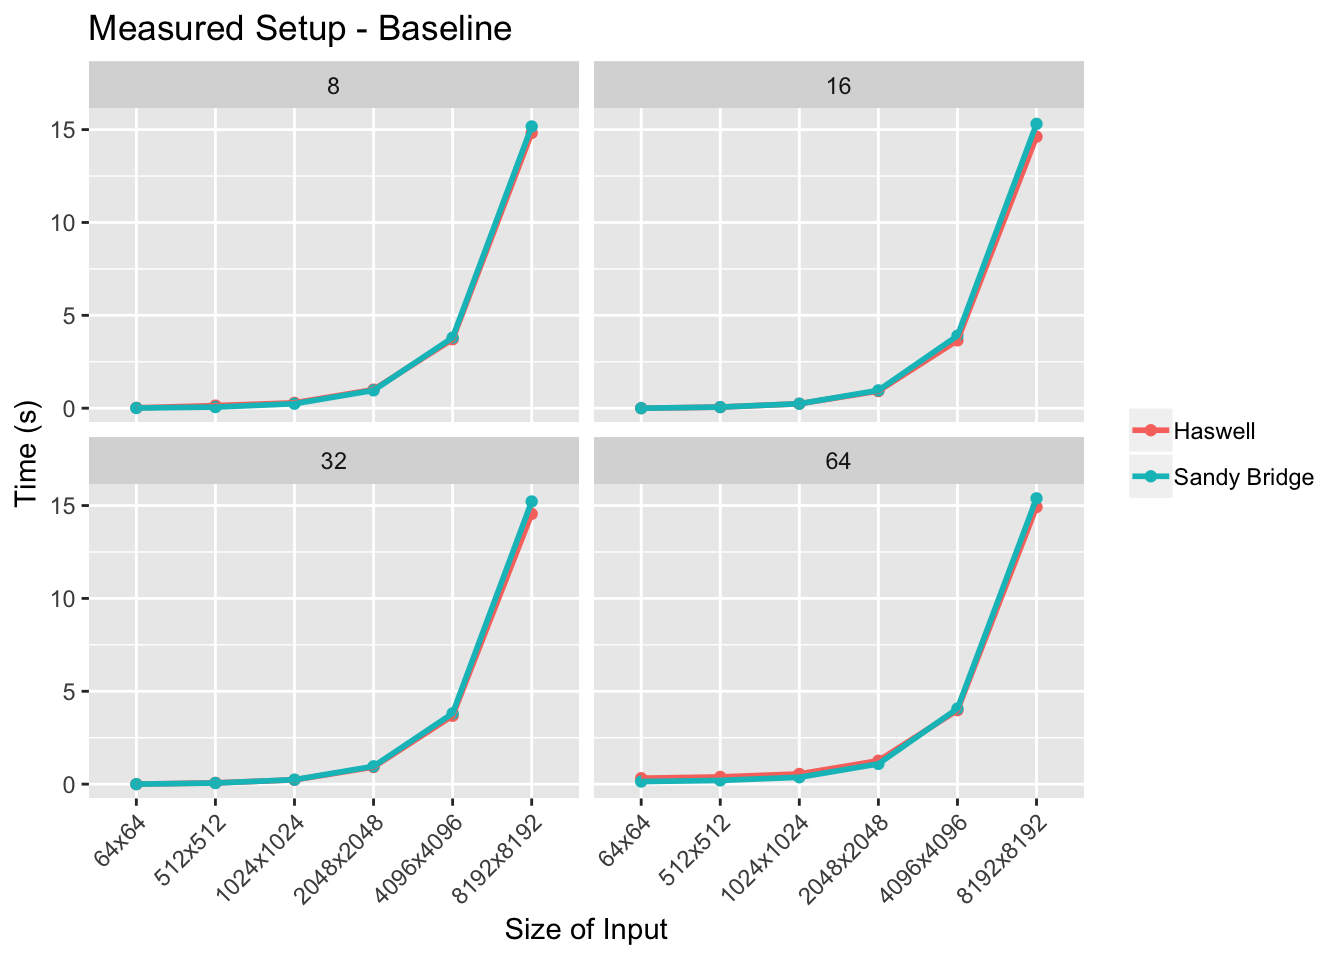
\includegraphics[scale = 0.18]{Baseline_Measured-Setup_Processes.png}
%\captionof{figure}{example code for adding pic} 
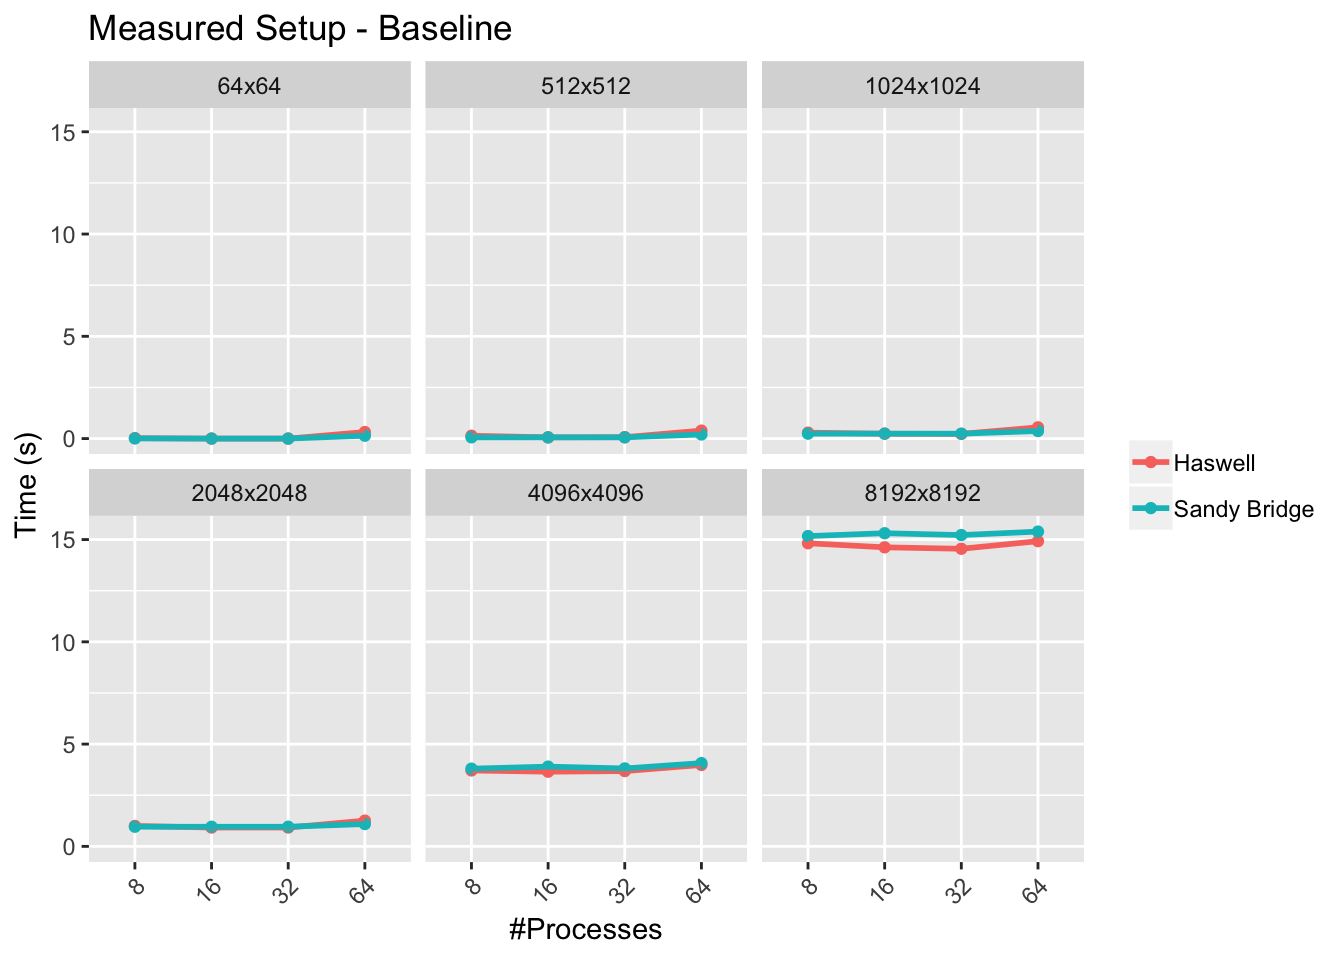
\includegraphics[scale = 0.18]{Baseline_Measured-Setup_InputSize.png}
%\captionof{figure}{example code for adding pic} 
\vspace{5mm}
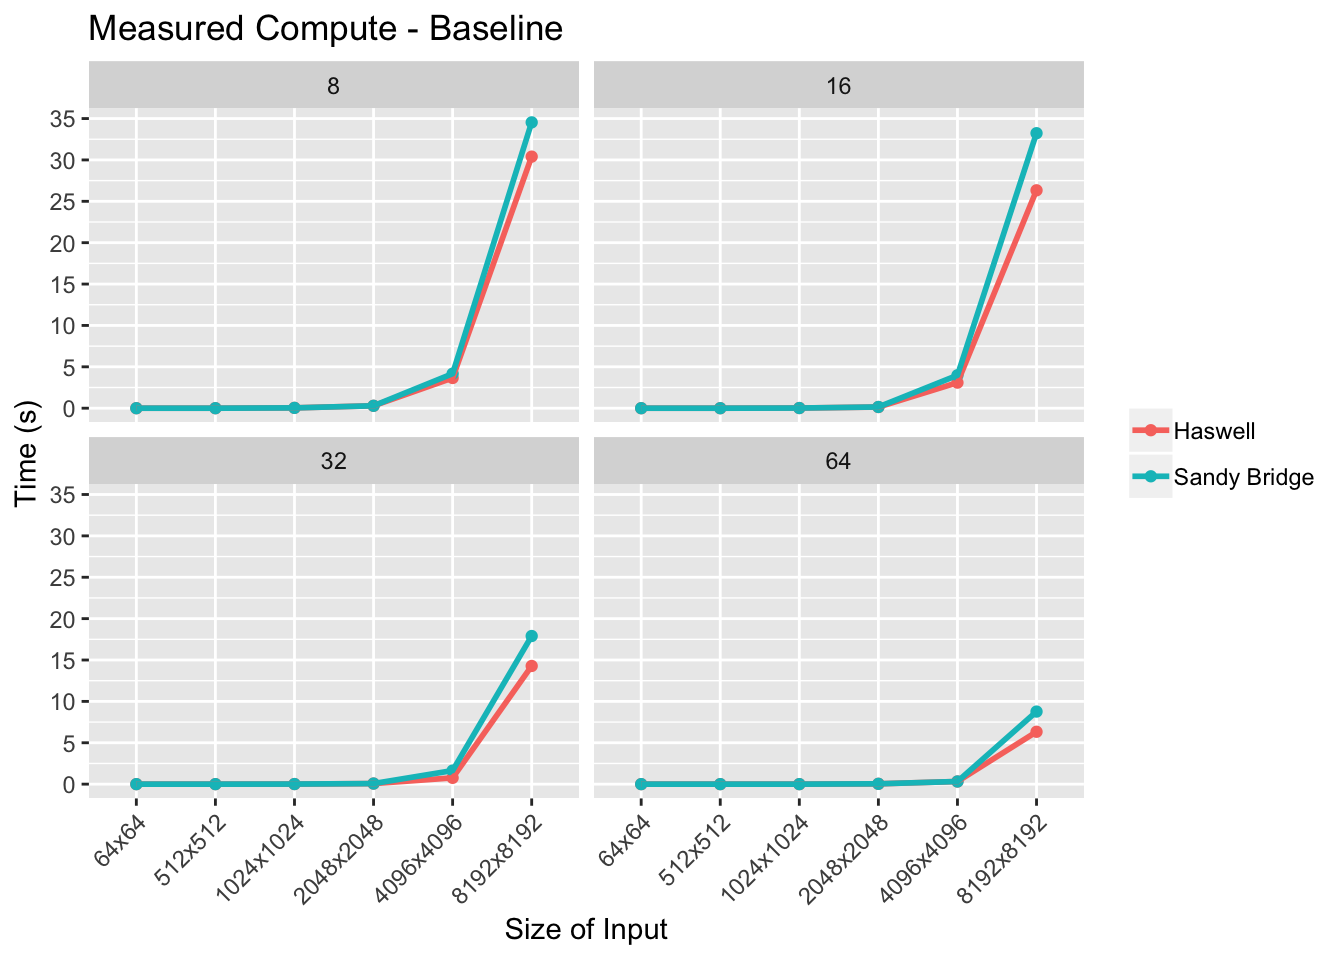
\includegraphics[scale = 0.18]{Baseline_Measured-Compute_Processes.png}
%\captionof{figure}{example code for adding pic} 
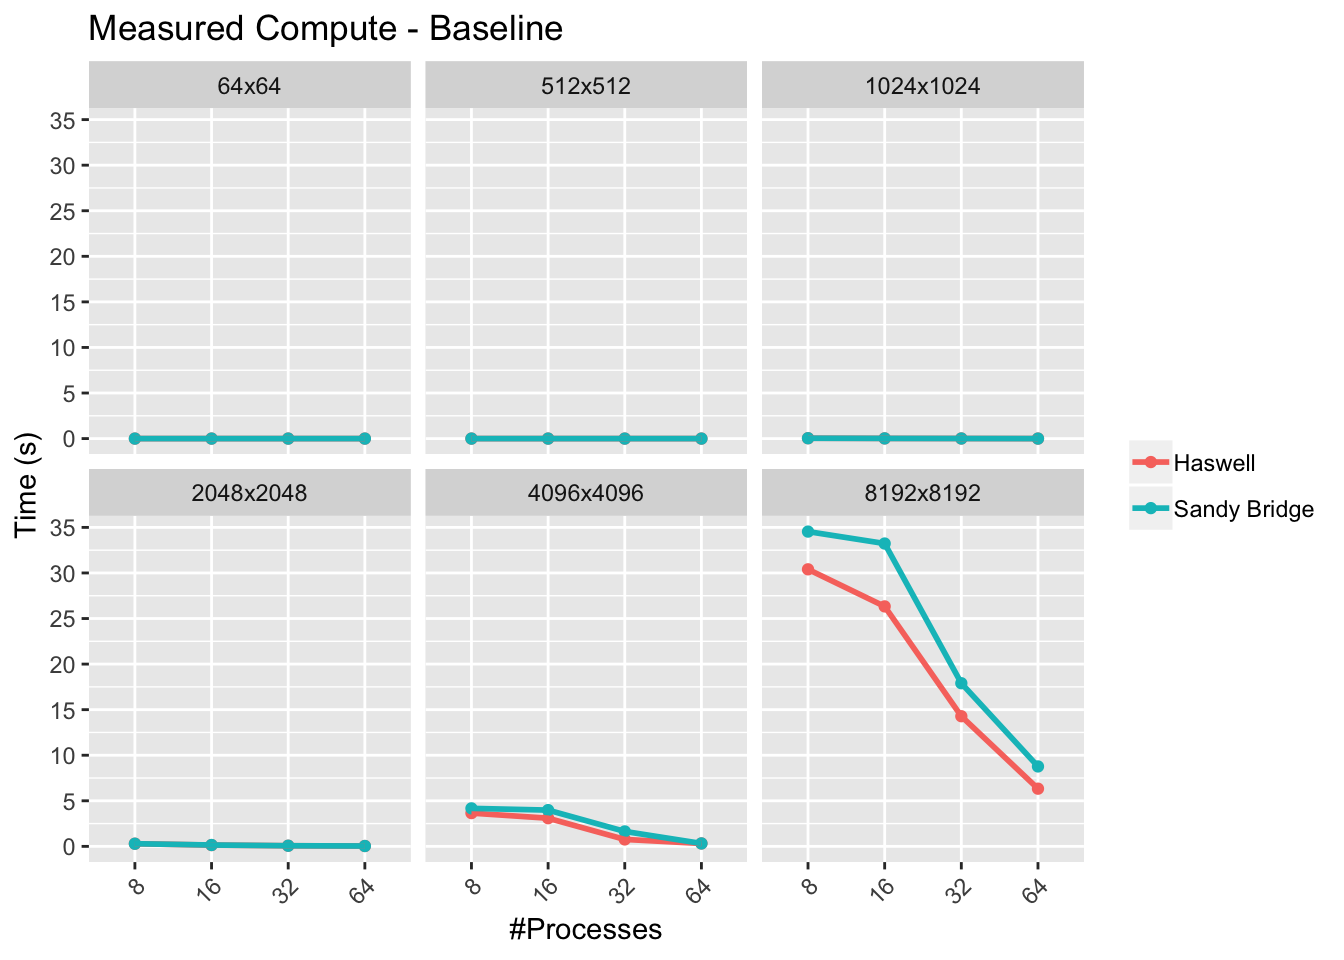
\includegraphics[scale = 0.18]{Baseline_Measured-Compute_InputSize.png}
%\captionof{figure}{example code for adding pic} 
\vspace{5mm}
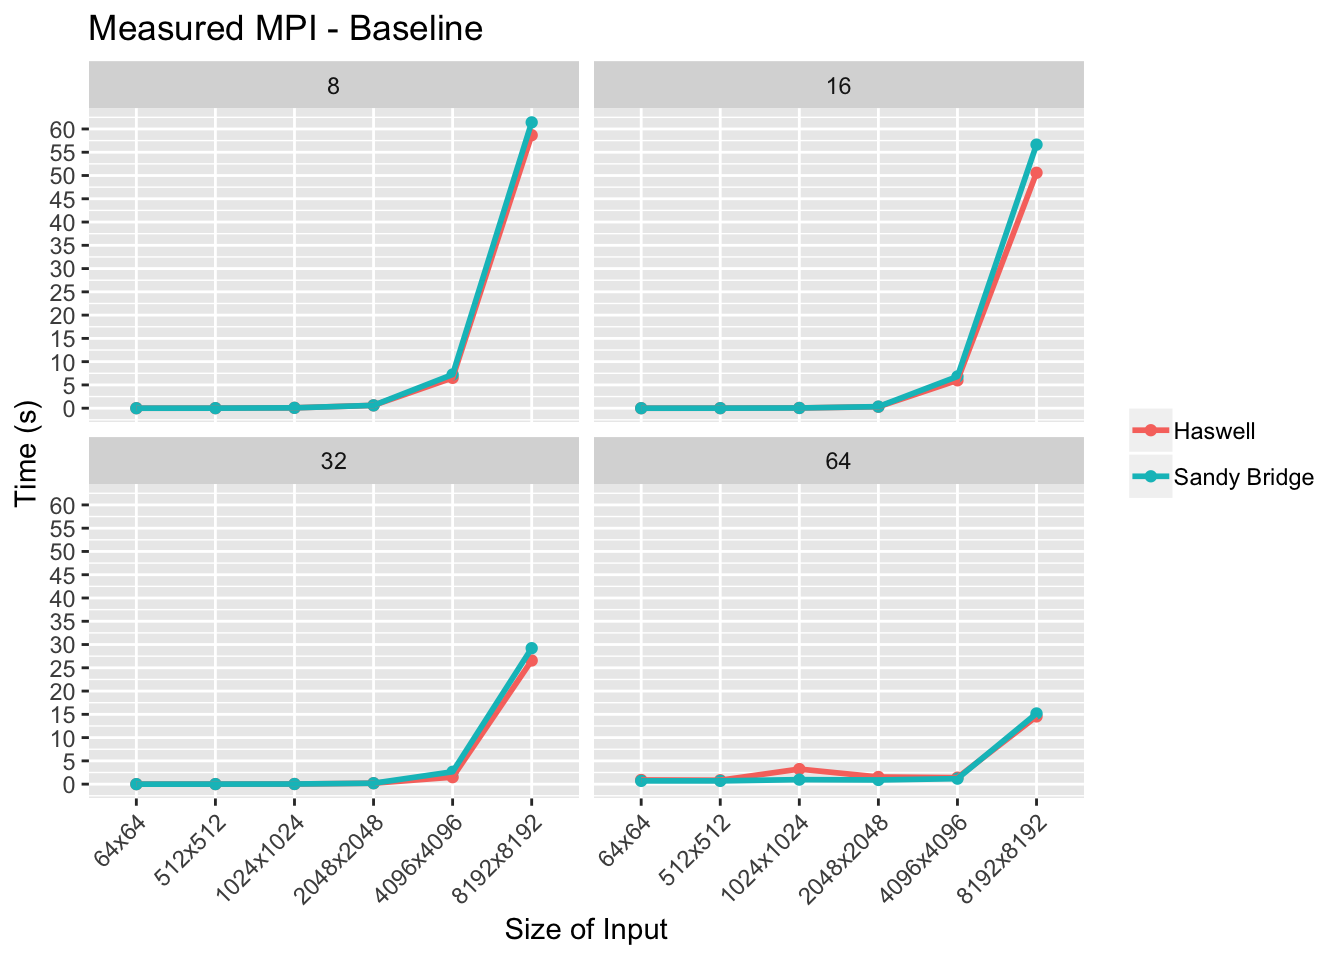
\includegraphics[scale = 0.18]{Baseline_Measured-MPI_Processes.png}
%\captionof{figure}{example code for adding pic} 
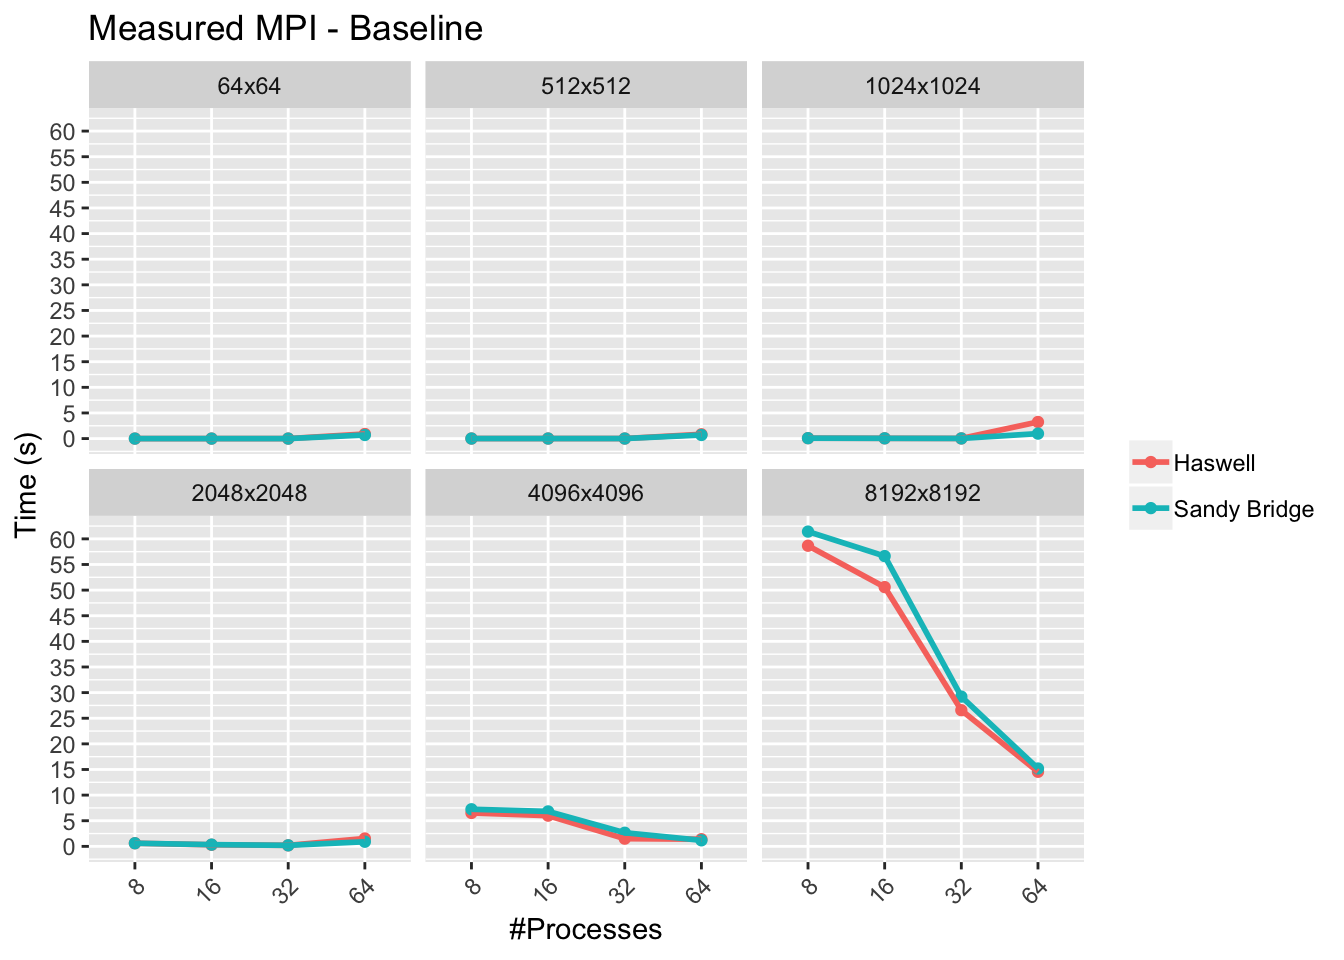
\includegraphics[scale = 0.18]{Baseline_Measured-MPI_InputSize.png}
%\captionof{figure}{example code for adding pic} 
\vspace{5mm}
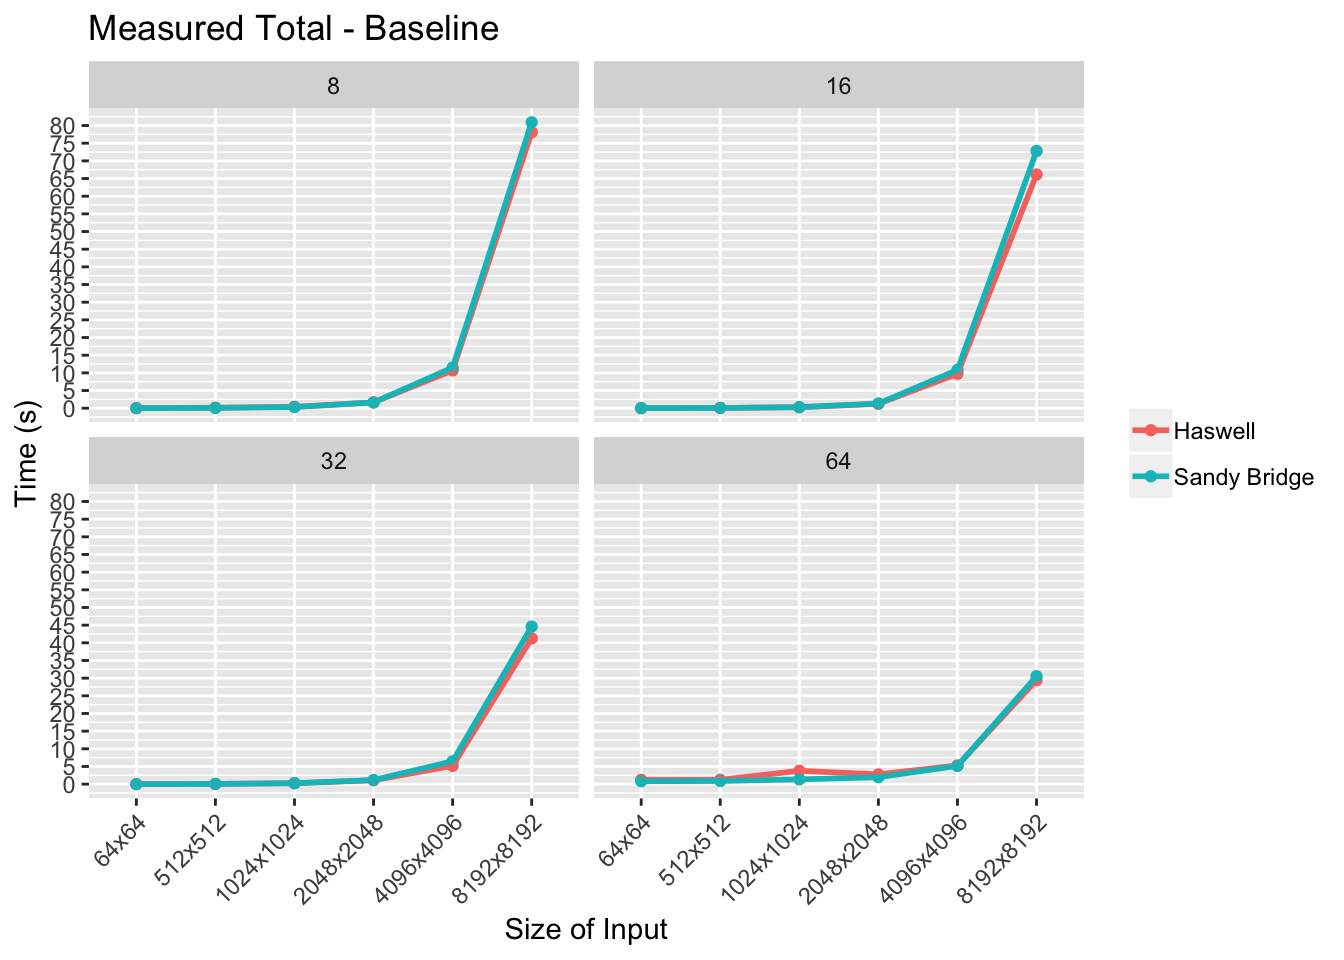
\includegraphics[scale = 0.18]{Baseline_Measured-Total_Processes.png}
%\captionof{figure}{example code for adding pic} 
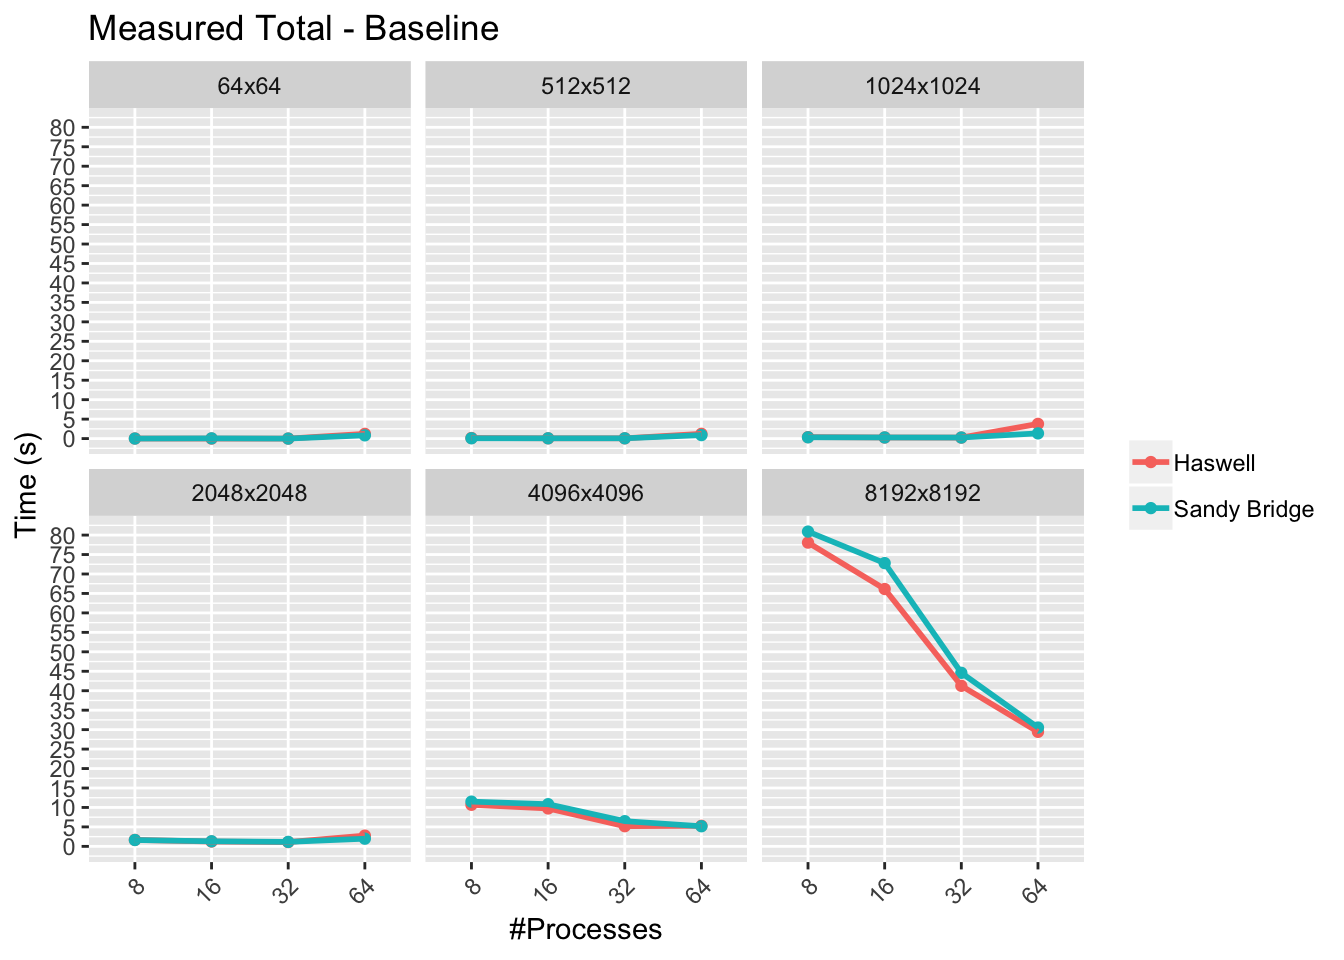
\includegraphics[scale = 0.18]{Baseline_Measured-Total_InputSize.png}
%\captionof{figure}{example code for adding pic} 

\end{enumerate} 

\subsection{Questions}

\begin{enumerate}
\item\textbf{Briefly describe the Gaussian Elimination and the provided implementation.} 

\url{[https://en.wikipedia.org/wiki/Gaussian_elimination]} \\	
Gaussian elimination (also known as row reduction) is an algorithm for solving systems of linear equations. It is usually understood as a sequence of operations performed on the corresponding matrix of coefficients. There are three steps of elementary row transformation:
\begin{enumerate}
\item{Swapping two rows}
\item{Multiplying a row by a nonzero number}
\item{Adding a multiple of one row to another row}
\end{enumerate}
Using these operations, a matrix can always be transformed into an upper triangular matrix. Our implementation divides the matrix into rows and then provides a set of them to each process. Each row performs the various operations mentioned above and sets the corresponding column values to zero thus resulting in a upper triangular matrix. 
	
\item\textbf{How is data distributed among the processes?} 

All the rows in the data should be divided equally among the processes in such a way that each of the process can take a max of row/processes number of rows of the matrix. 

\item \textbf{Explain the changes applied to the provided Load-Leveler batch script.} 

To address the variance between the runs, we ran each of the instance multiple times. For each combination of processes and input file size, the job was executed 3 times to find an average value.

\item \textbf{What were the challenges in getting an accurate baseline time for Gaussian Elimination.} 

To get accurate baseline time for Gaussian Elimination, we had to ensure less waiting time for each of the measured times. The factors affecting the various measured times are explained as follows. IO communication takes place sequentially, so the number of processes does not affect the time. Setup time is the time required by each process to receive the rows of the matrix. From the performance plots, we observe that setup time increases with increase in domain input size. Also, even for high number of processes, the setup time is low for lower domain size. Setup time is relatively constant when processes is increased keeping domain size constant. This may probably be due to communication overhead. Compute time measures the time interval between the start and end of gaussian elimination. It also includes the MPI time. Compute time should be constant for a domain size even though number of processes increase. MPI time is communication time. MPI time increases with increase domain size and for 1024 domain size, it decreases with increase in processes. Total time is time required for entire Gaussian elimination algorithm to execute.  

\item\textbf{Describe the compute and MPI times scalability with fixed process counts and varying size of input files for the Sandy Bridge and Haswell nodes. Did you observe any differences?}
 
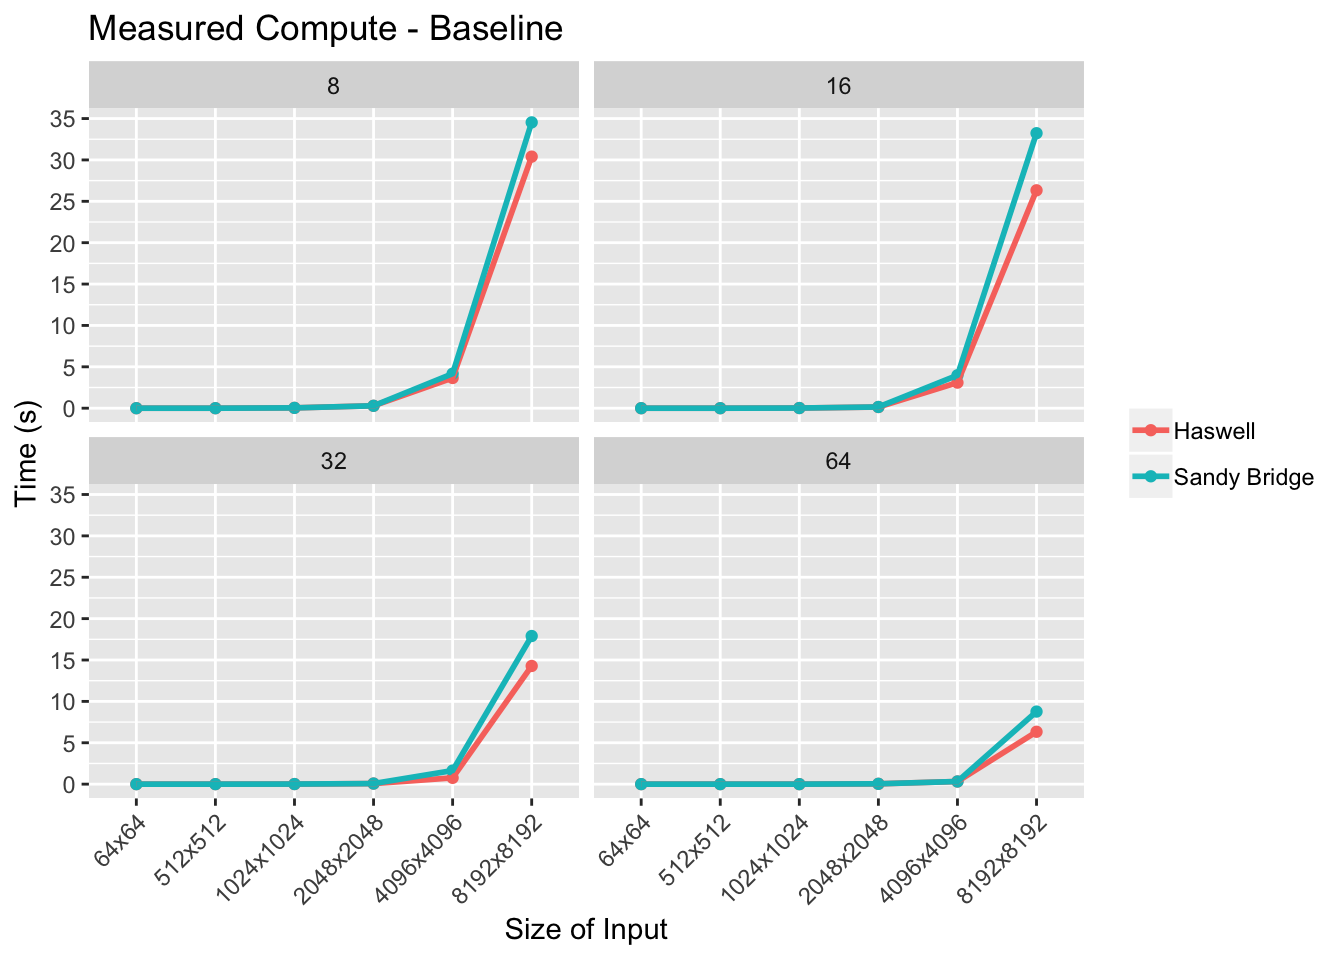
\includegraphics[scale = 0.18]{Baseline_Measured-Compute_Processes.png}
%\captionof{figure}{example code for adding pic} 
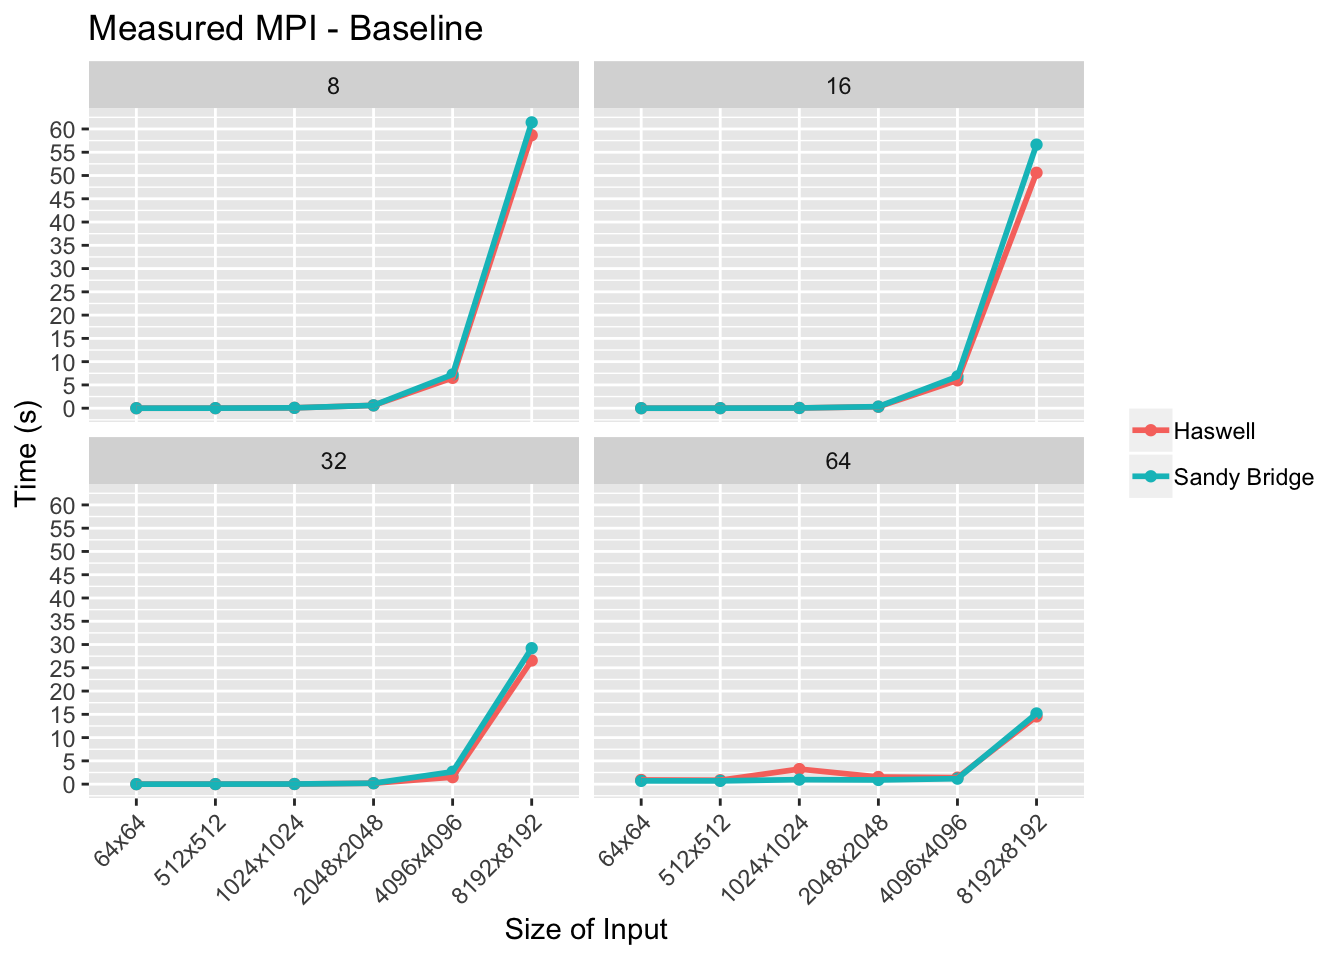
\includegraphics[scale = 0.18]{Baseline_Measured-MPI_Processes.png}
%\captionof{figure}{example code for adding pic} 
\\
With fixed process count and a varying size of input files, we observe that the compute time increases with input size. When comparing the performance of the Haswell and Sandy Bridge architectures, we observe that Haswell nodes generally have less compute times compared to Sandy Bridge when the domain size is between 2048 and 8192. However, the Sandy Bridge nodes have less compute times at small domain sizes.

At the same time, MPI time increases with domain size. We also see that Haswell nodes have shorter MPI times compared to Sandy Bridge nodes for when the domain size is above 4096. When the domain size is below 4096, Sandy Bridge nodes have shorter MPI times for all process count 64. Thus we observe that, the Haswell nodes perform slightly better. 

\item\textbf{Describe the compute and MPI times scalability with fixed input sets and varying process counts for the Sandy Bridge and Haswell nodes. Did you observe any differences?} 

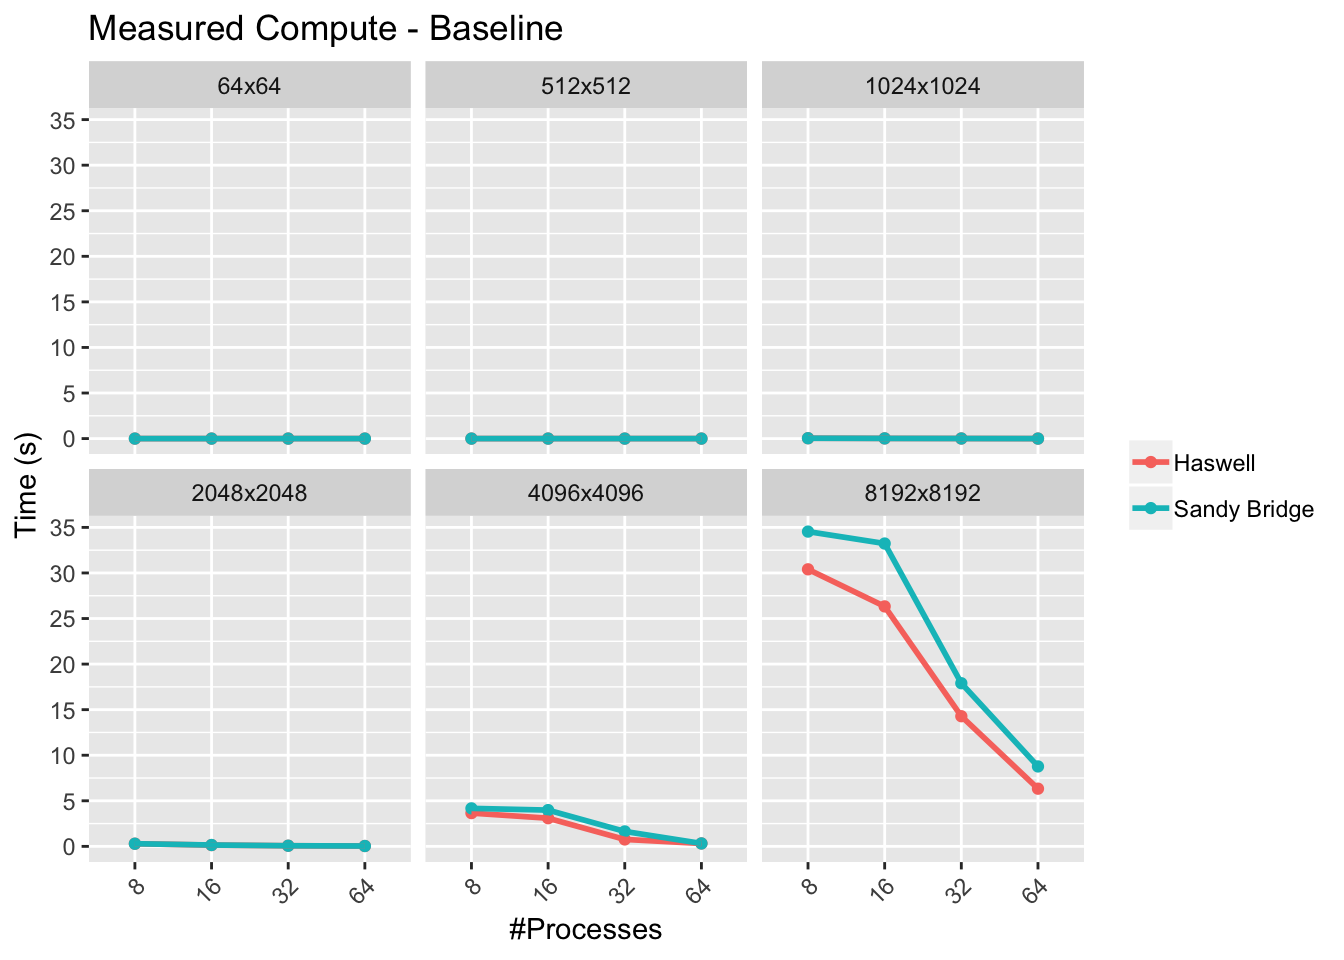
\includegraphics[scale = 0.18]{Baseline_Measured-Compute_InputSize.png}
%\captionof{figure}{example code for adding pic} 
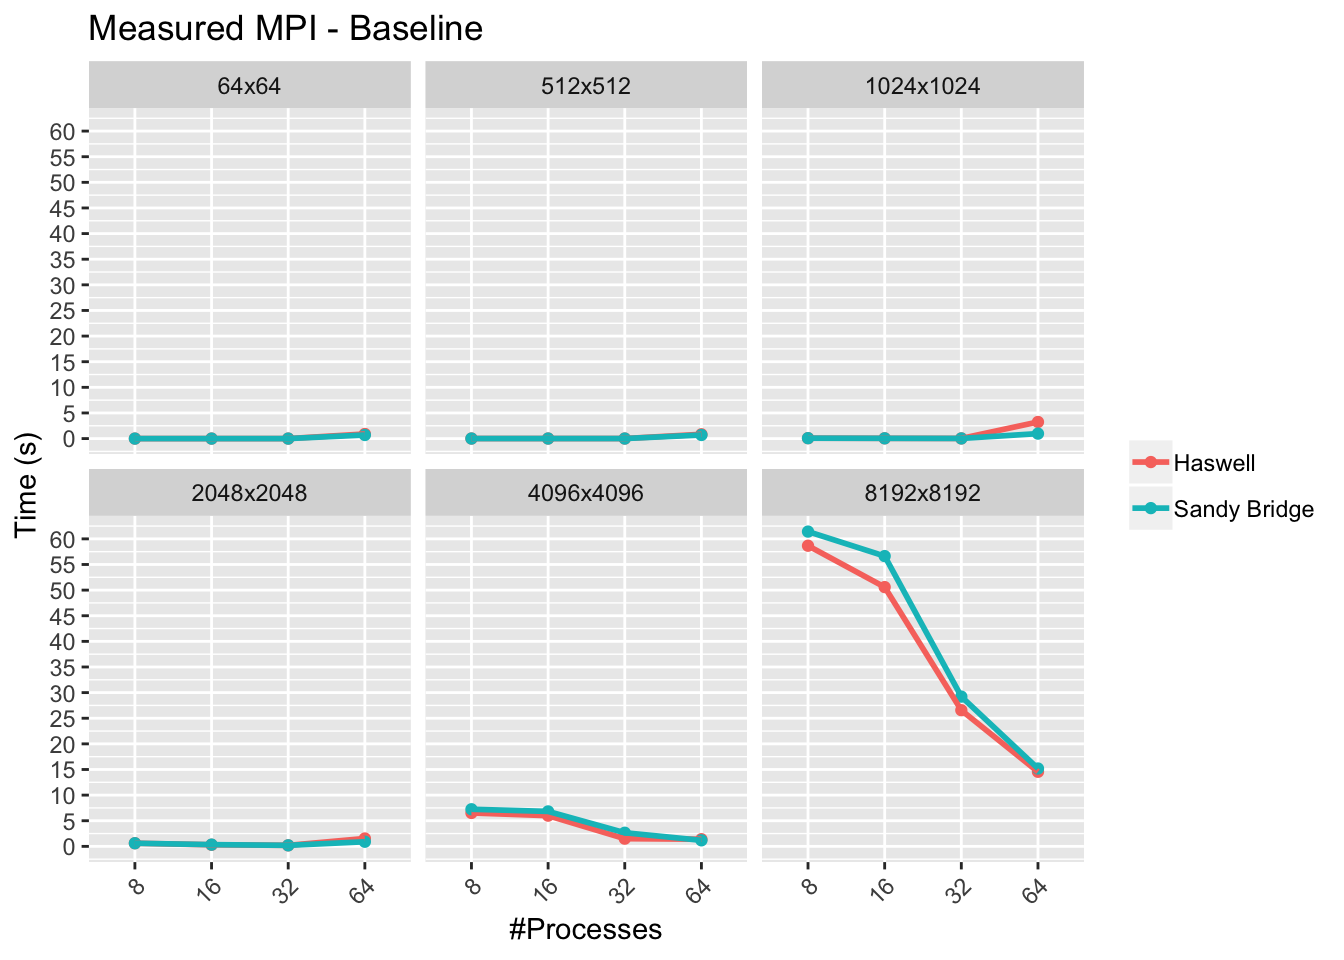
\includegraphics[scale = 0.18]{Baseline_Measured-MPI_InputSize.png}
%\captionof{figure}{example code for adding pic} 
\\
With fixed input size and increasing the process count, we observe that the compute time decreases with process count.The compute time is completely negligible in comparison to the communication time for small input size of 64. At higher domain size, we see that the Haswell nodes has comparatively shorter compute times for any processor count. However, the Sandy Bridge nodes still seem to scale better with a larger number of processes at a large domain size.

For smaller domain size, MPI time is longer as number of processes increase. But for larger domain size, the MPI time decreases and we observe Haswell has comparatively less MPI time than Sandy Bridge as processes increase. Overall, Haswell has better performance architecture. 

\end{enumerate}

\section{MPI Point-to-Point Communication}

\subsection{Required submission files}

\begin{enumerate}
\item \textbf{The updated gauss.c file.} 

Refer gauss\_nonblock.c file from code scripts of Task 4.1   

\item \textbf{The new performance plots and the description in the report.} 

The various performance plots for MPI Point-to-Point communication are: \\
\\
%\vspace{5mm}
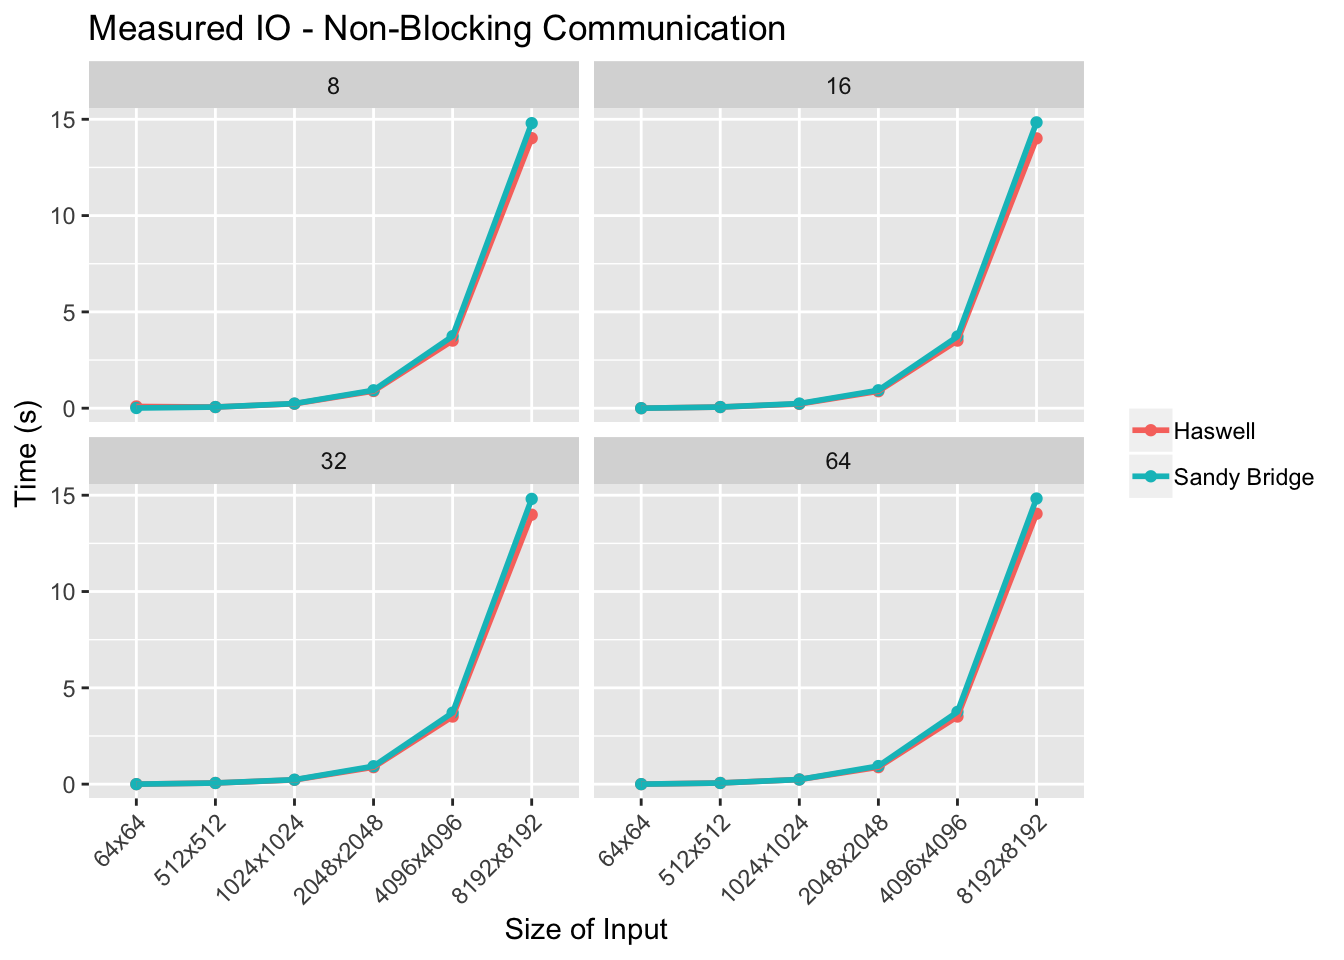
\includegraphics[scale = 0.18]{P2P_Measured-IO_Processes.png}
%\captionof{figure}{example code for adding pic} 
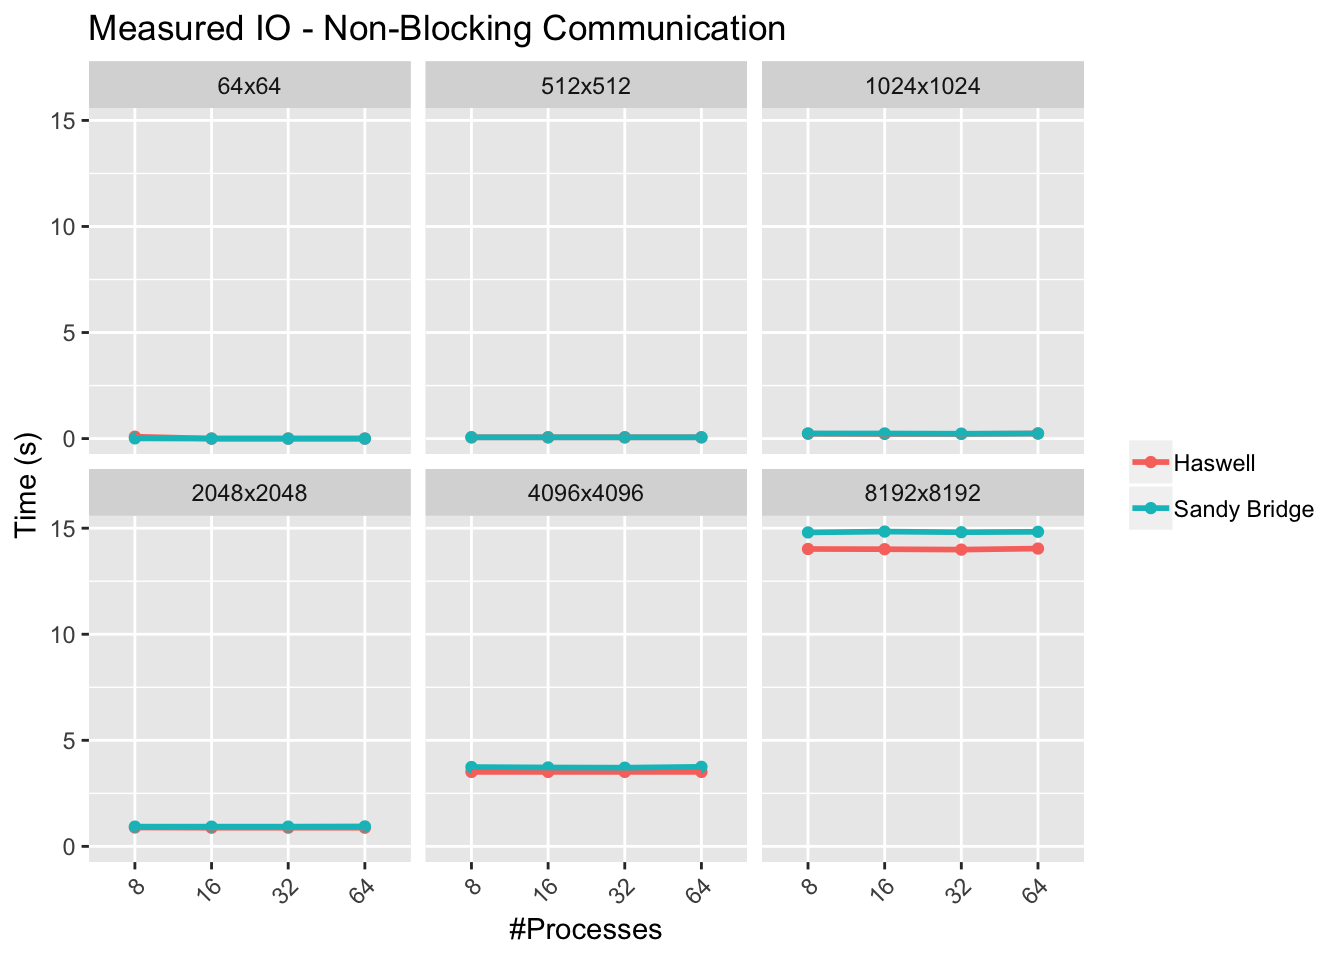
\includegraphics[scale = 0.18]{P2P_Measured-IO_InputSize.png}
%\captionof{figure}{example code for adding pic} 
\vspace{2mm}
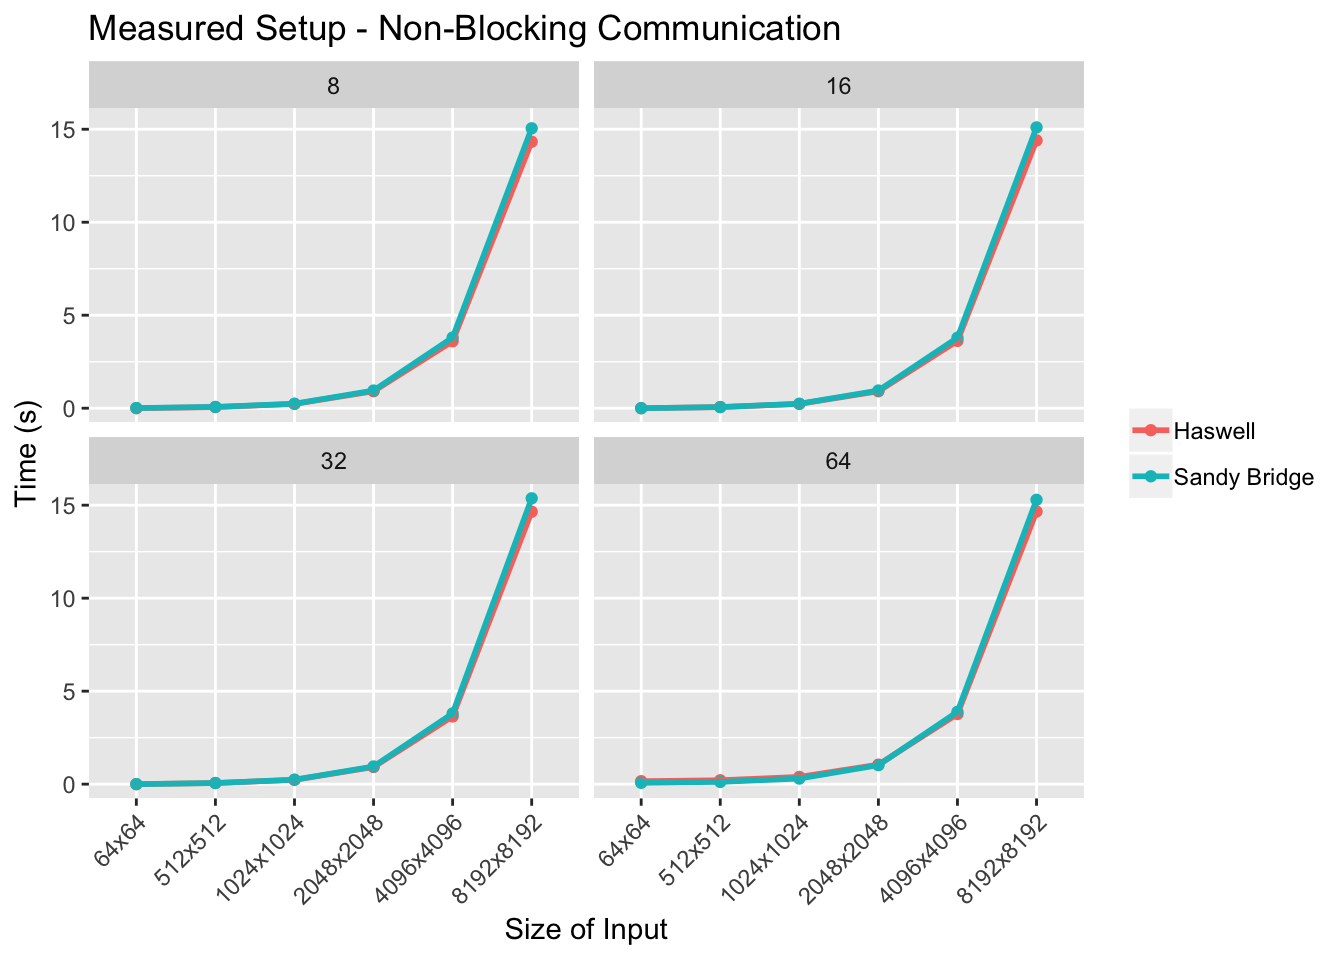
\includegraphics[scale = 0.18]{P2P_Measured-Setup_Processes.png}
%\captionof{figure}{example code for adding pic} 
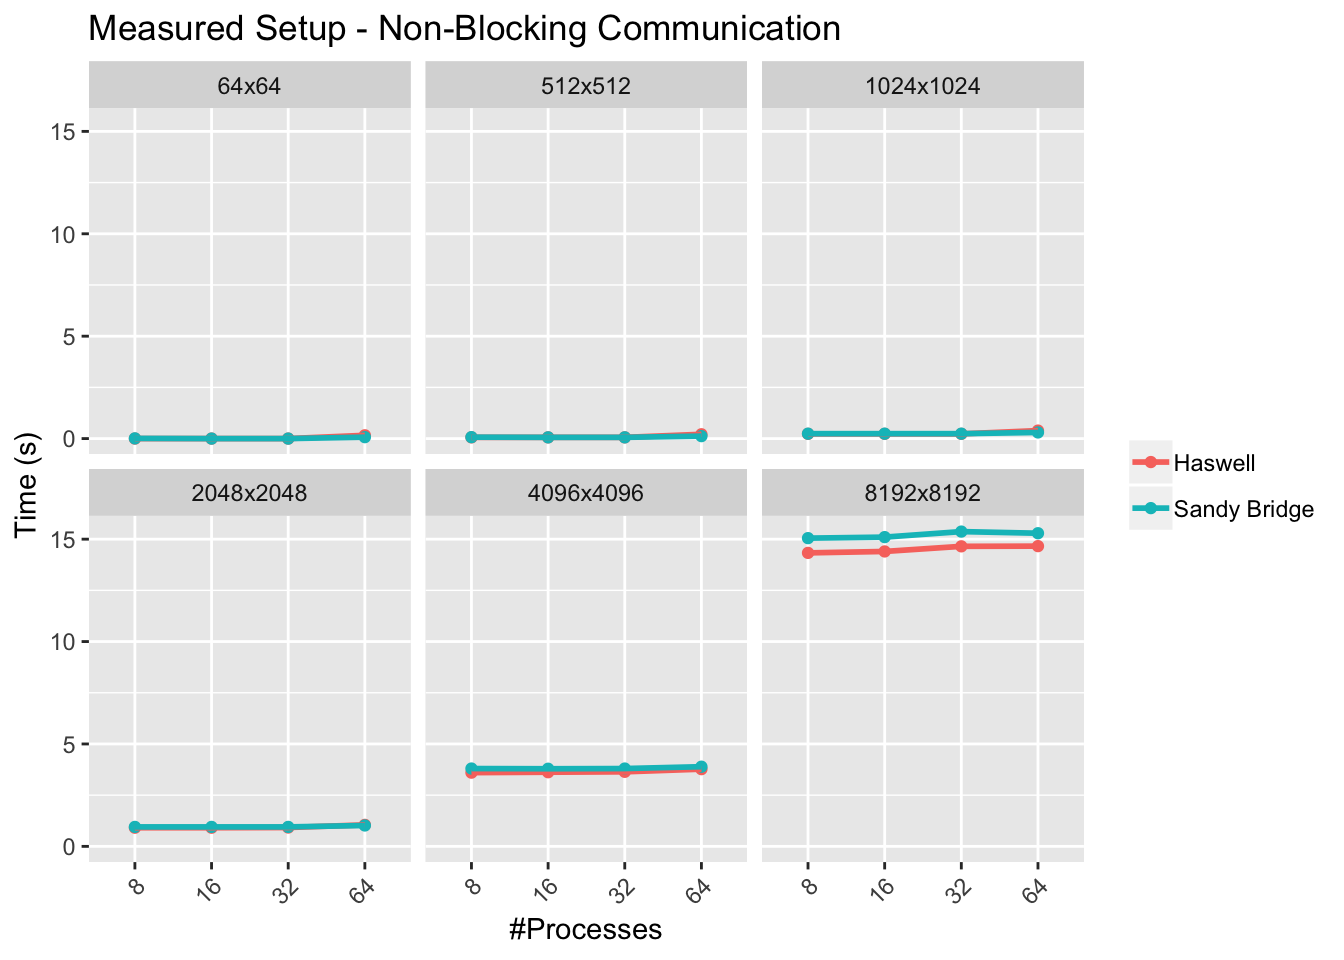
\includegraphics[scale = 0.18]{P2P_Measured-Setup_InputSize.png}
%\captionof{figure}{example code for adding pic} 
\vspace{5mm}
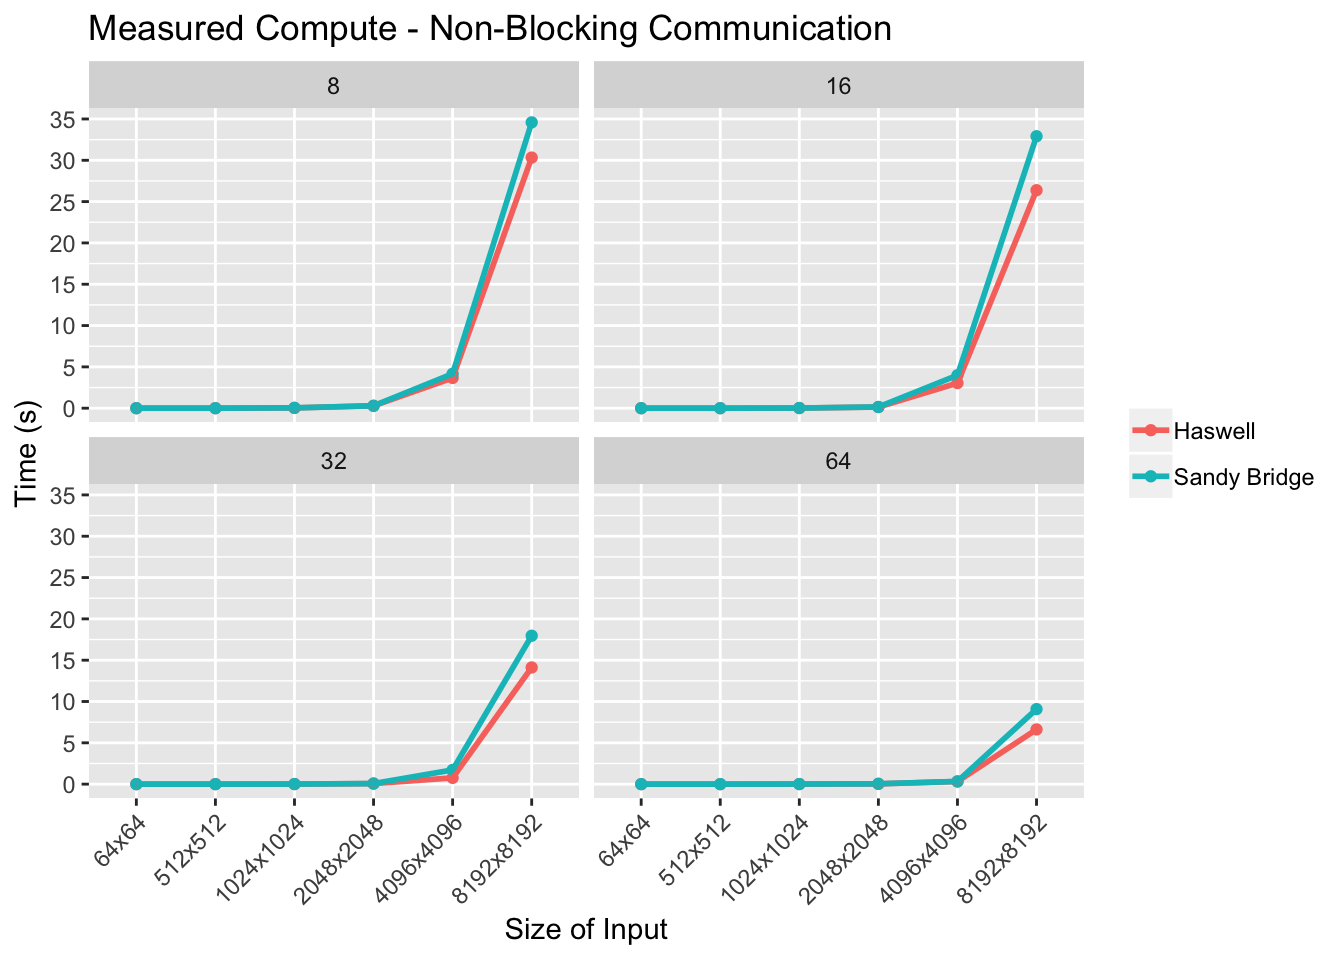
\includegraphics[scale = 0.18]{P2P_Measured-Compute_Processes.png}
%\captionof{figure}{example code for adding pic} 
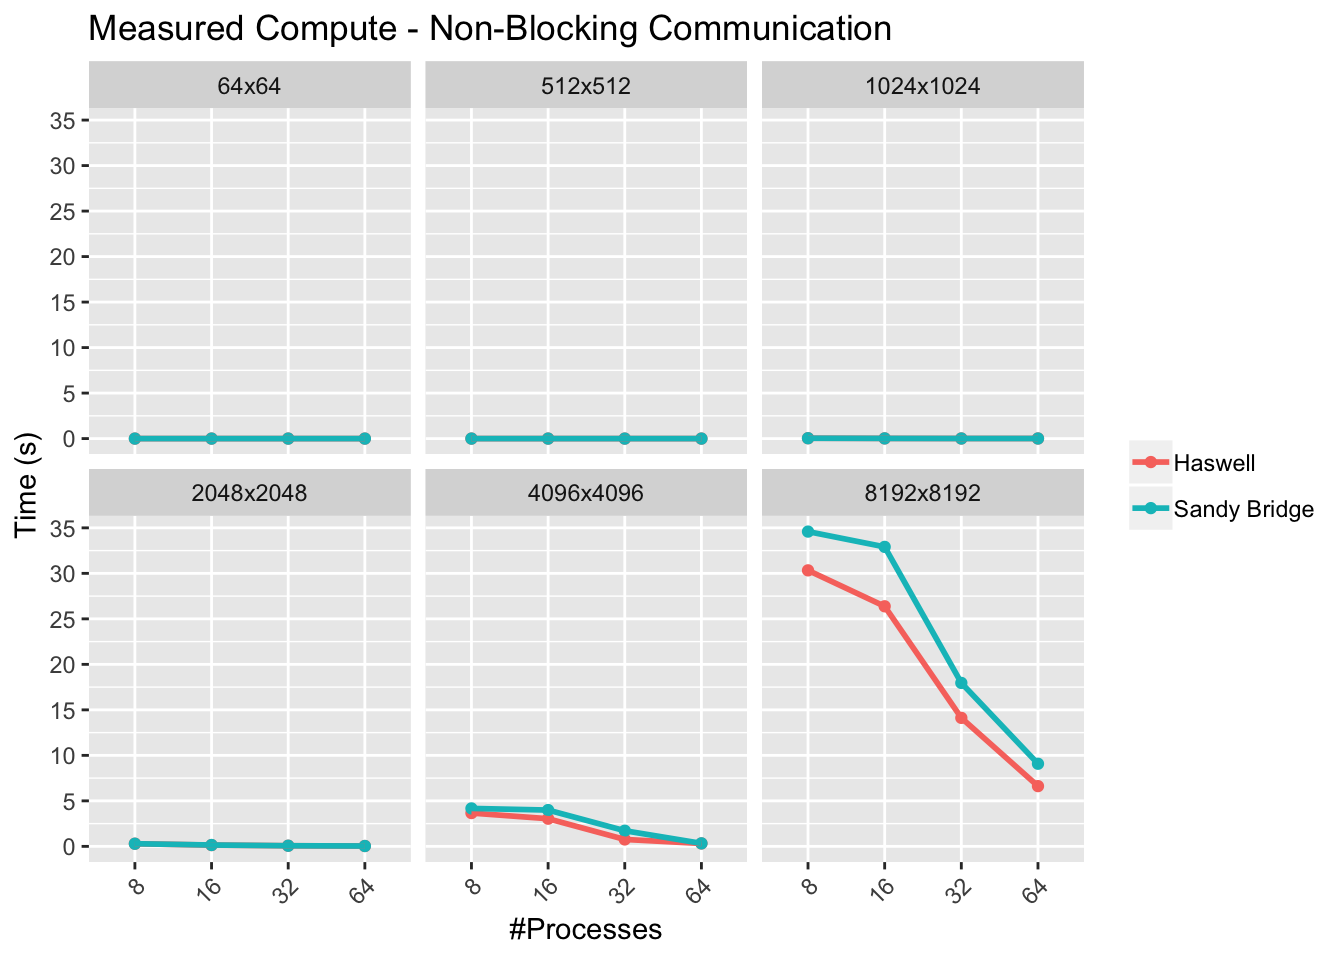
\includegraphics[scale = 0.18]{P2P_Measured-Compute_InputSize.png}
%\captionof{figure}{example code for adding pic} 
\vspace{5mm}
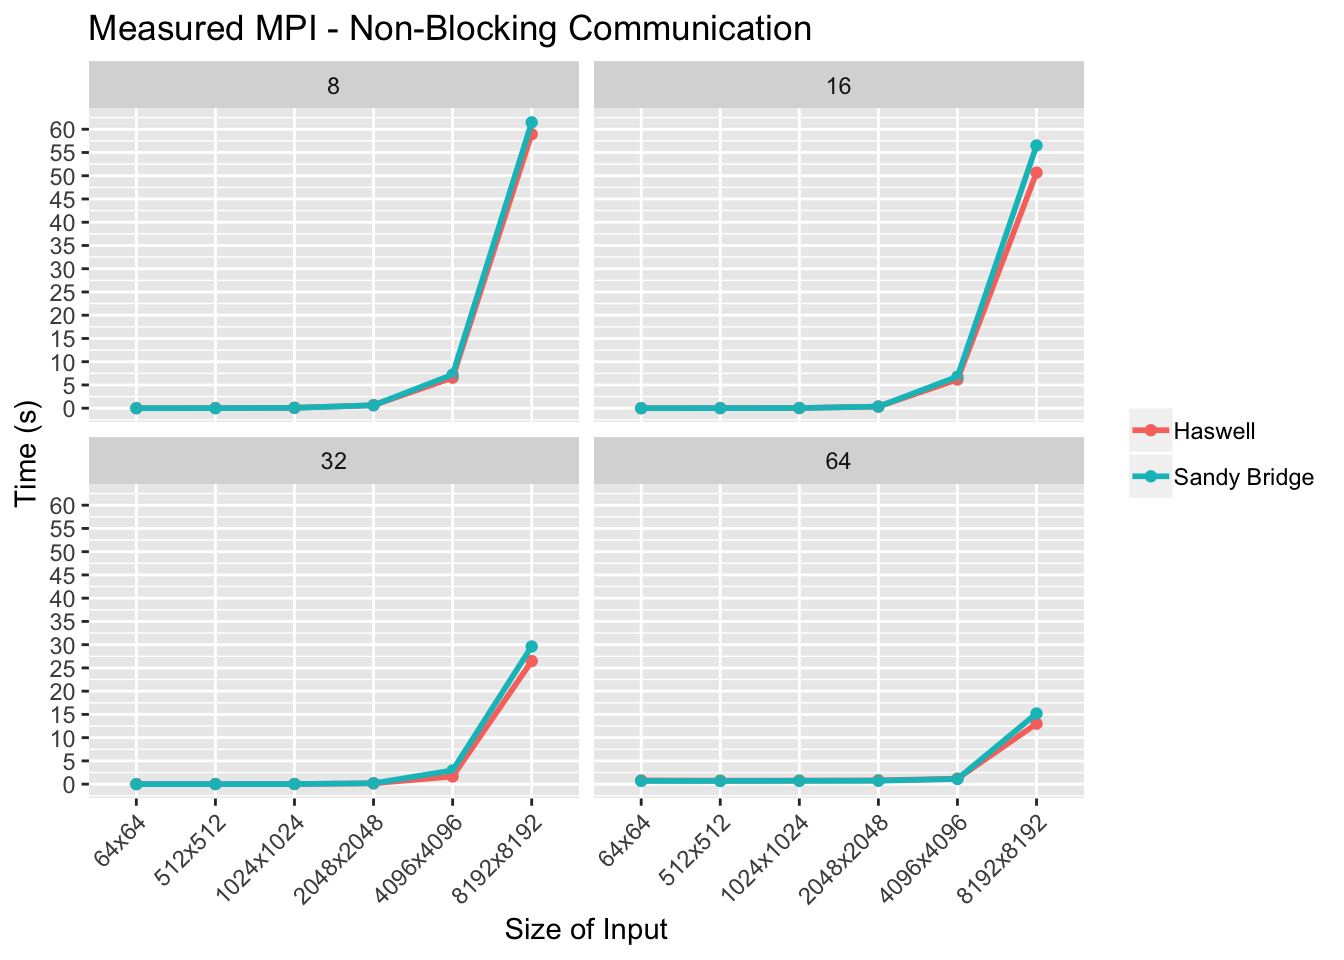
\includegraphics[scale = 0.18]{P2P_Measured-MPI_Processes.png}
%\captionof{figure}{example code for adding pic} 
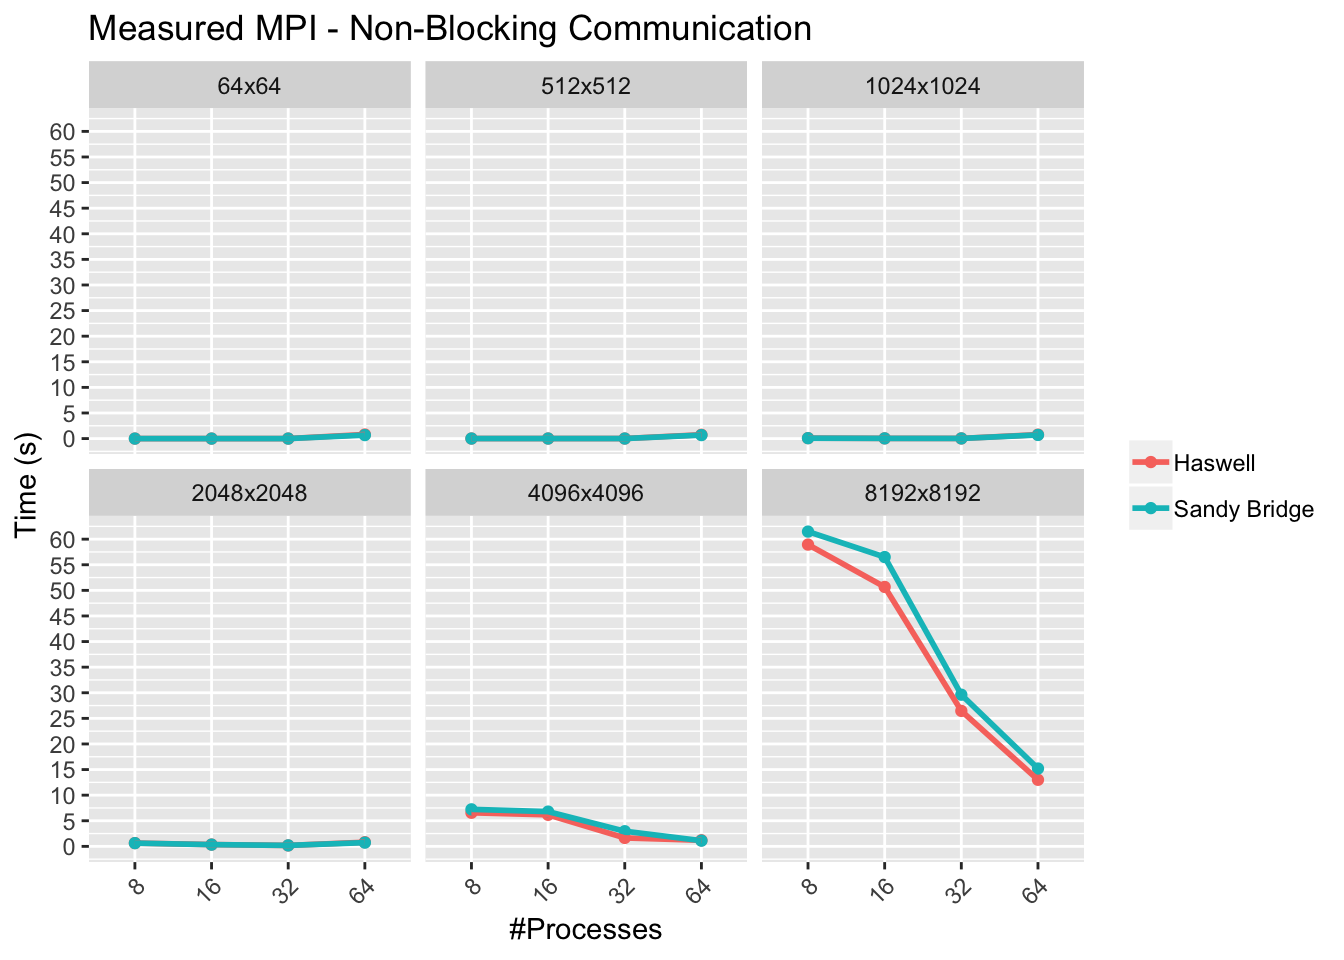
\includegraphics[scale = 0.18]{P2P_Measured-MPI_InputSize.png}
%\captionof{figure}{example code for adding pic} 
\vspace{5mm}
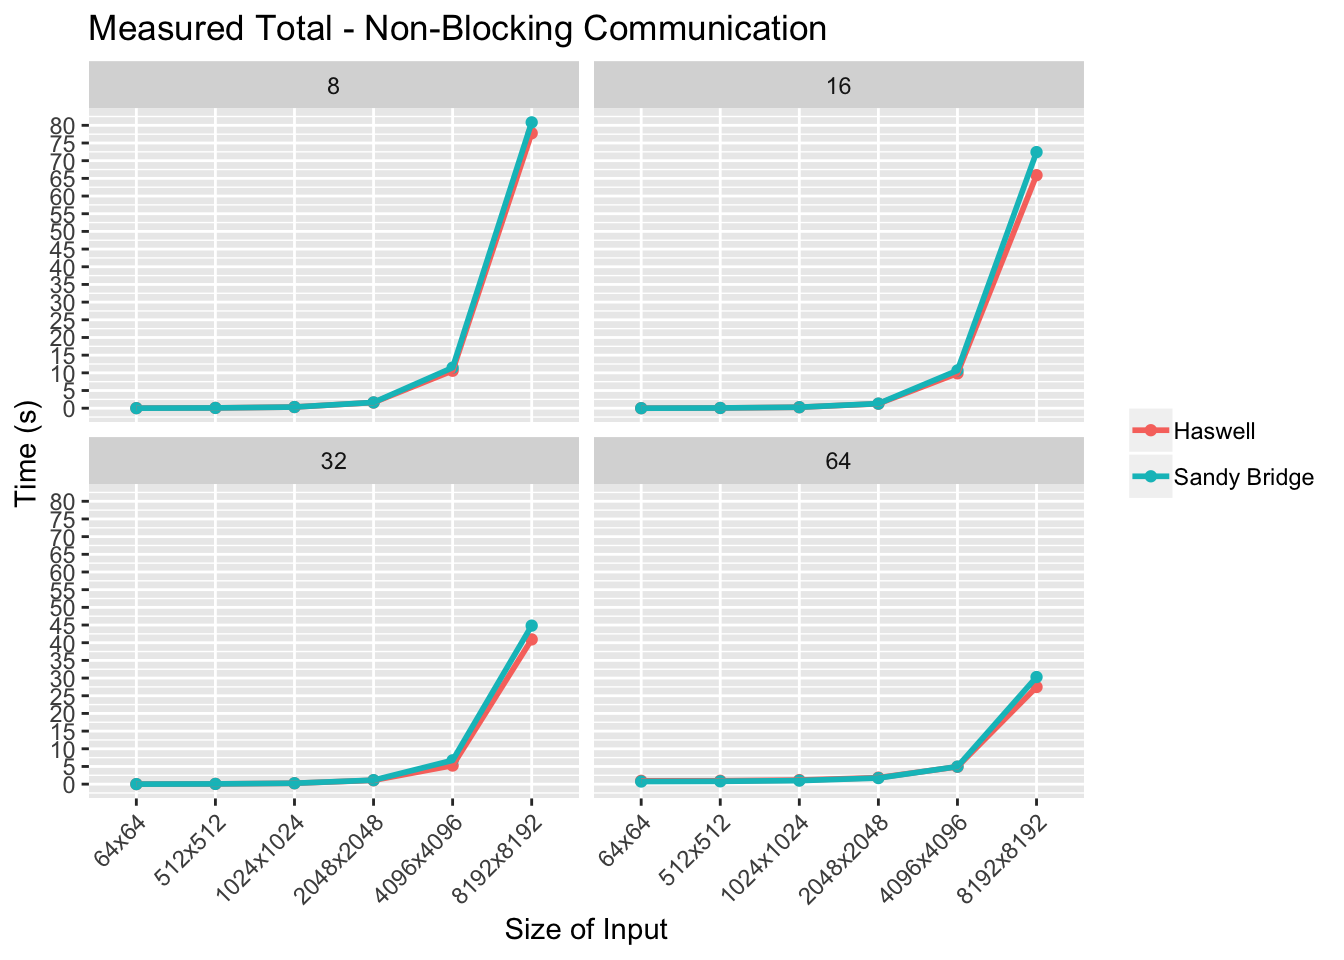
\includegraphics[scale = 0.18]{P2P_Measured-Total_Processes.png}
%\captionof{figure}{example code for adding pic} 
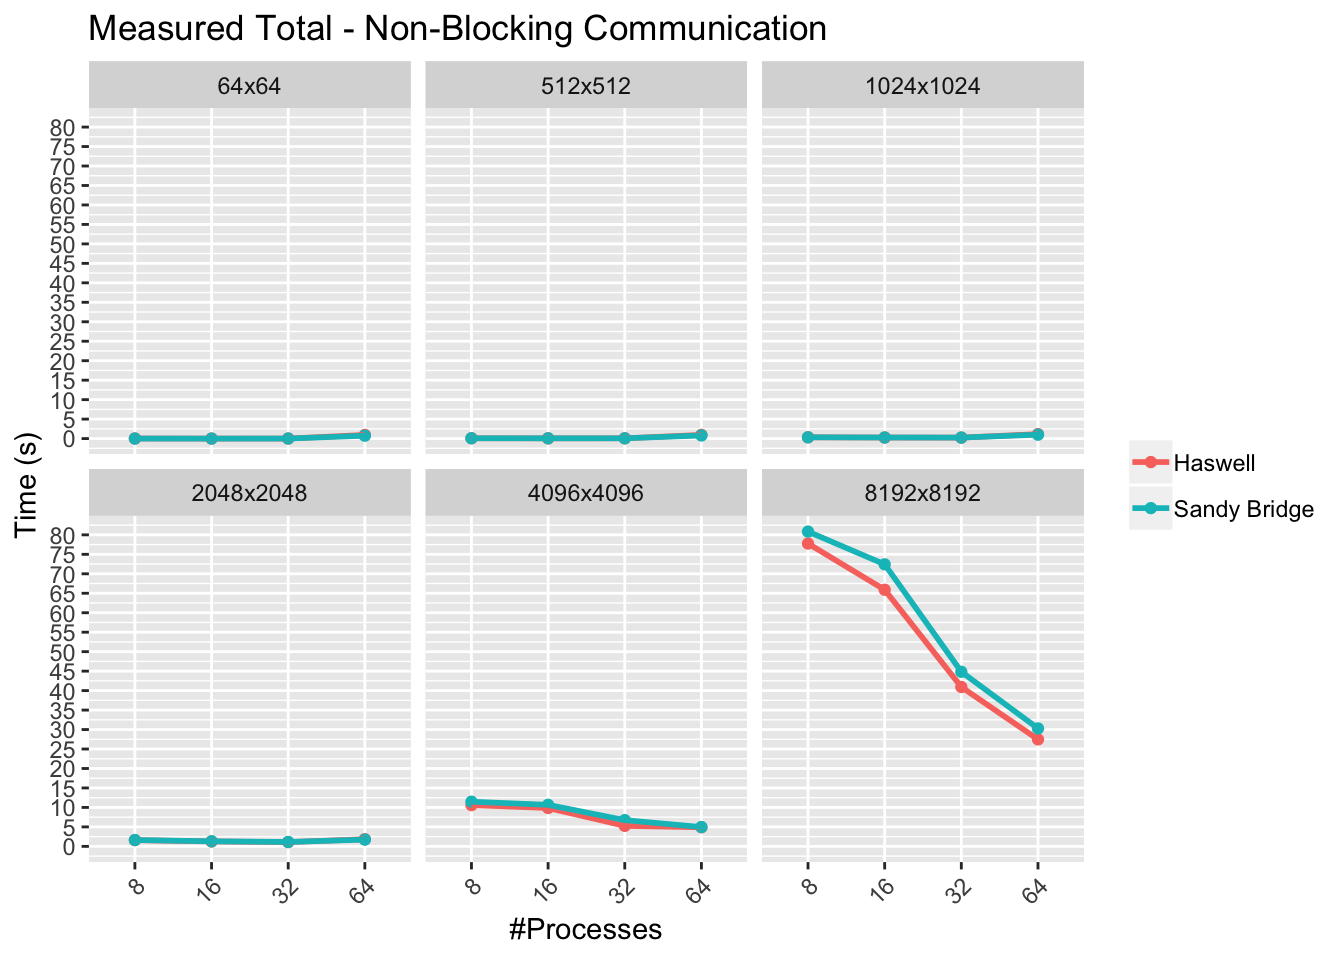
\includegraphics[scale = 0.18]{P2P_Measured-Total_InputSize.png}
%\captionof{figure}{example code for adding pic} 

\end{enumerate} 

\subsection{Questions}

\begin{enumerate}
\item\textbf{Which non-blocking operations were used? Justify your choice.} 
	
The non-blocking operations selected were \verb!MPI_Isend! and \verb!MPI_Irecv!. They seemed to provide the most amount of overlap, though its less than expected. \verb!MPI_Isend! was used to initiate the computation independent of whether data is received or not and thus reduce the waiting time. \verb!MPI_Irecv! was used to try to anticipate the communication.
    
\item\textbf{Was communication and computation overlap achieved? Use Vampir.} 
	
Communication and computation overlap was achieved, but not as much wanted. This can be observed from the below vampir plots. Some overlap done thanks to Isend but no Irecv as communication was performed for following loop iteration while computing the current one.

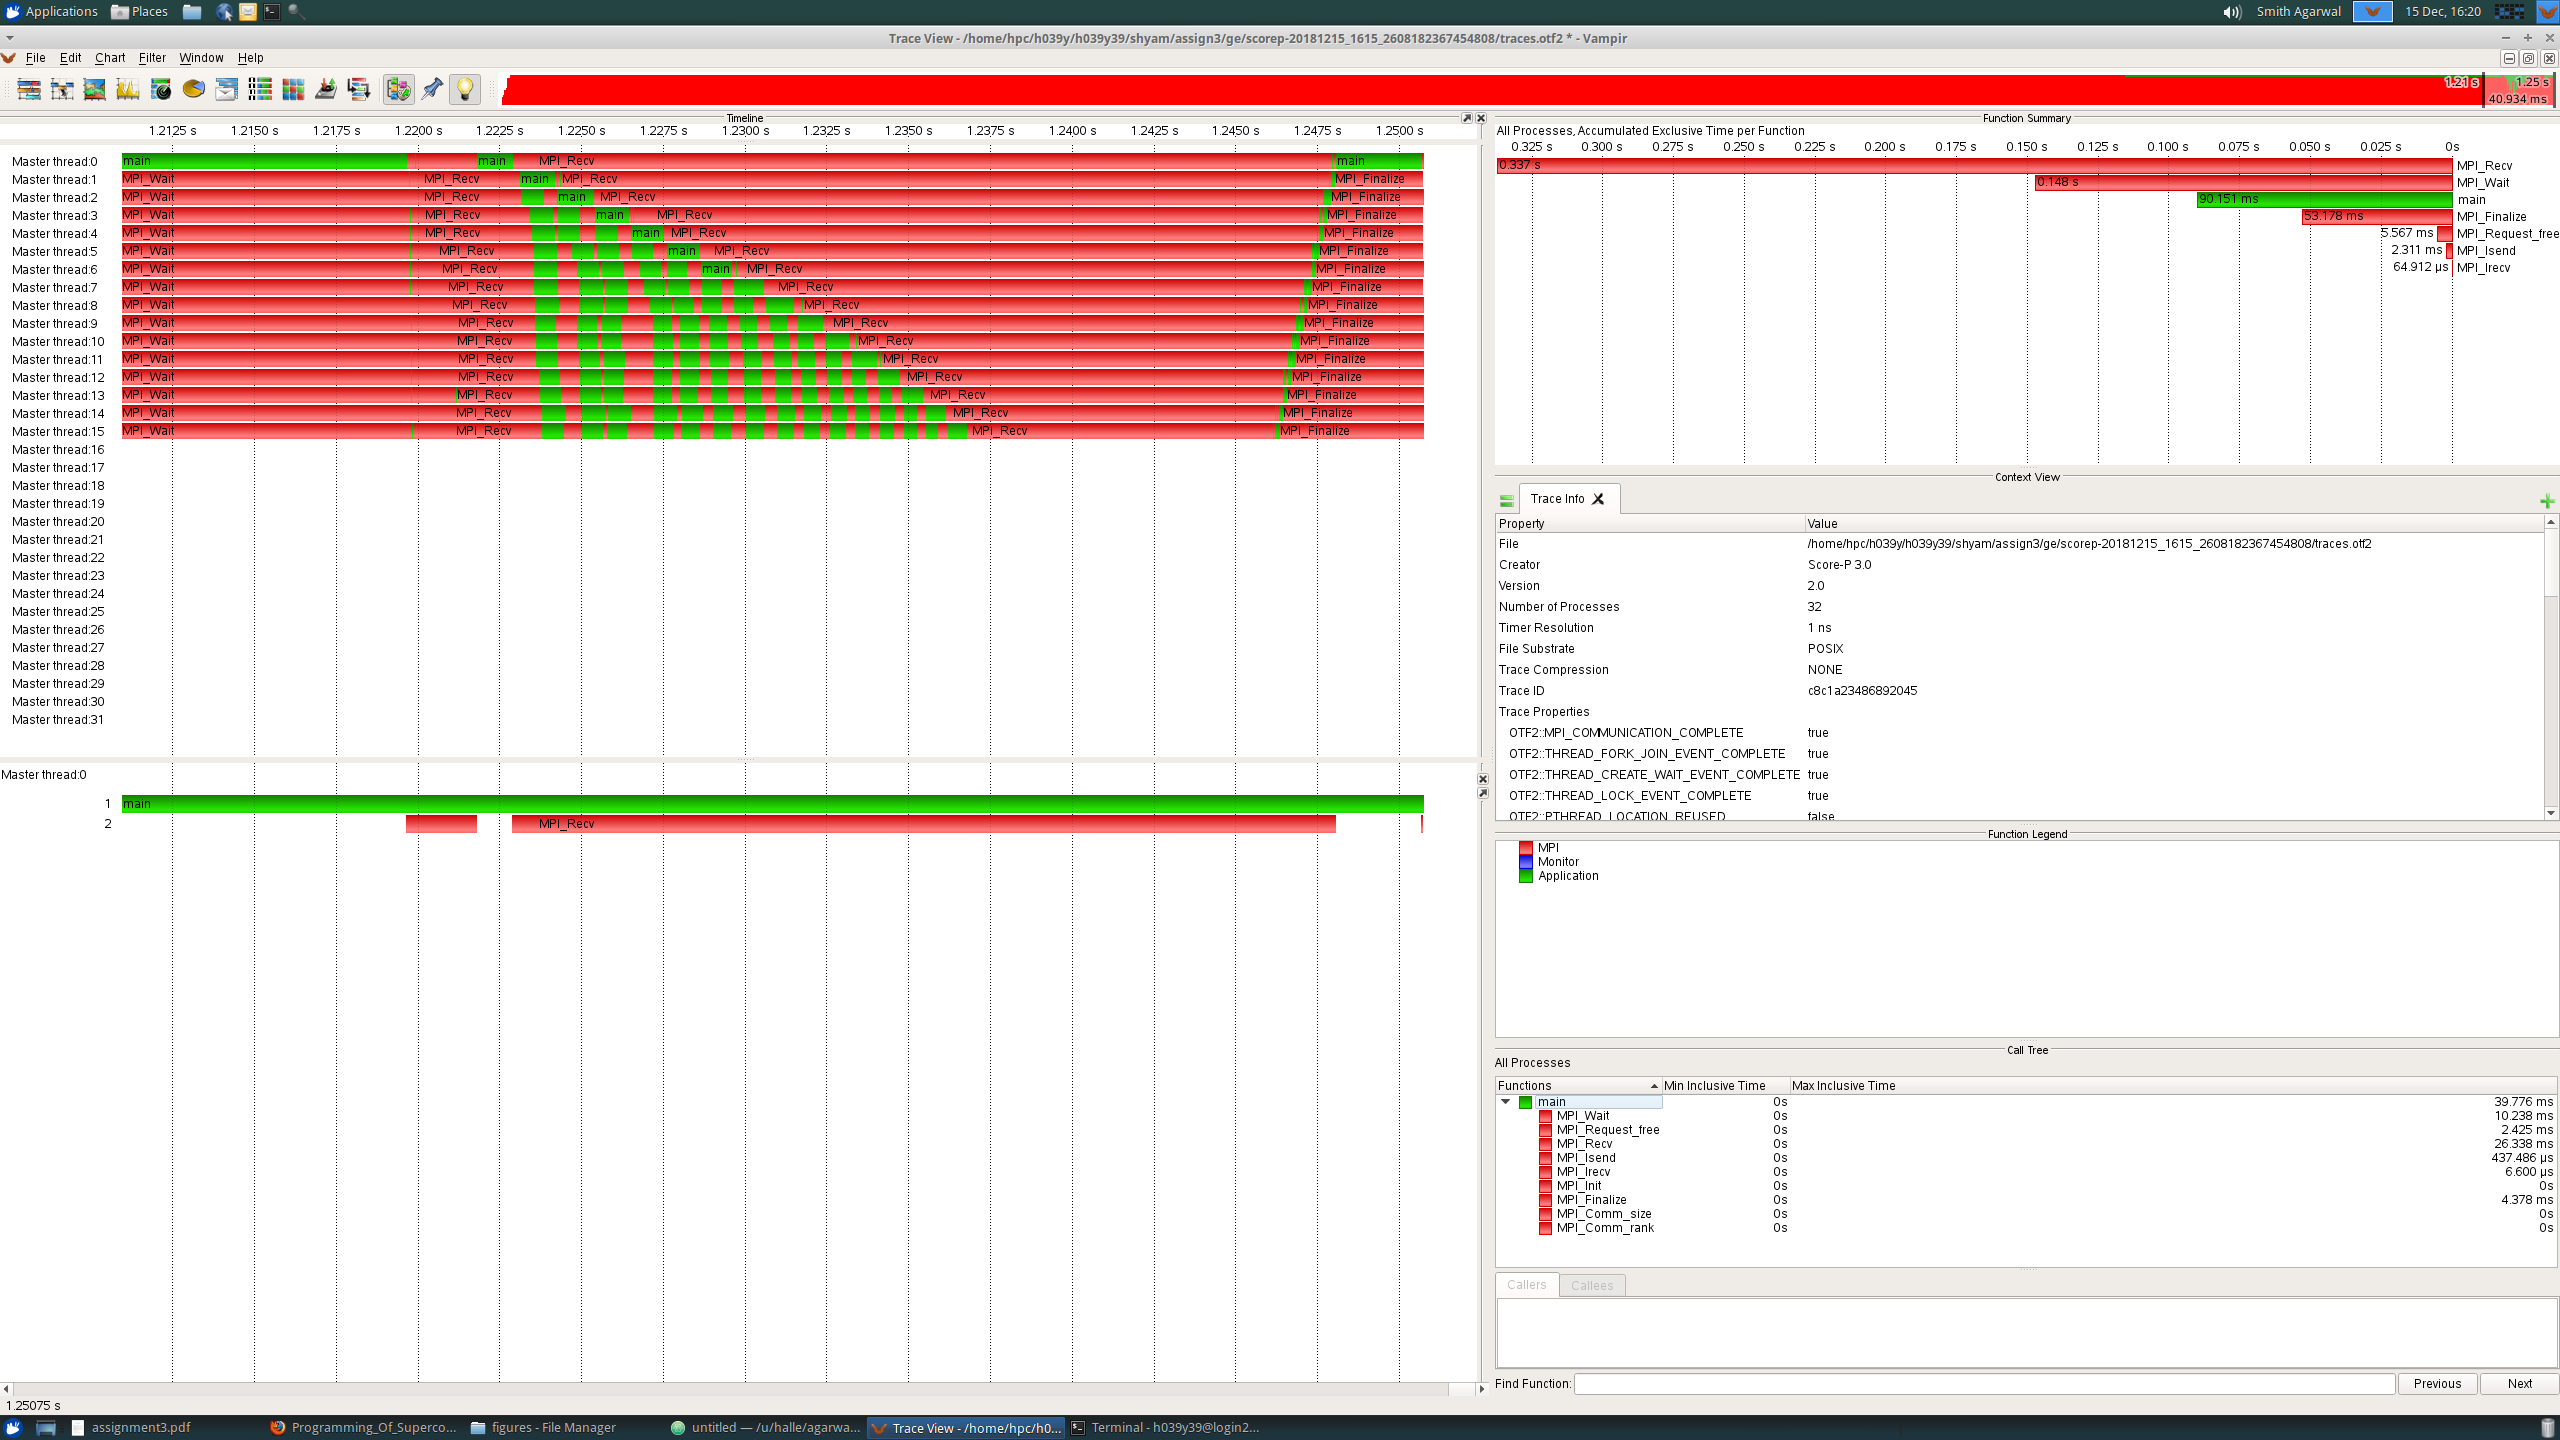
\includegraphics[scale = 0.16]{hw_nonblock_3.png}
\captionsetup{labelformat=empty}
\captionof{figure}{Figure : Vampir output for Point-to-point Haswell} 
\vspace{5mm}
\hspace{7mm}
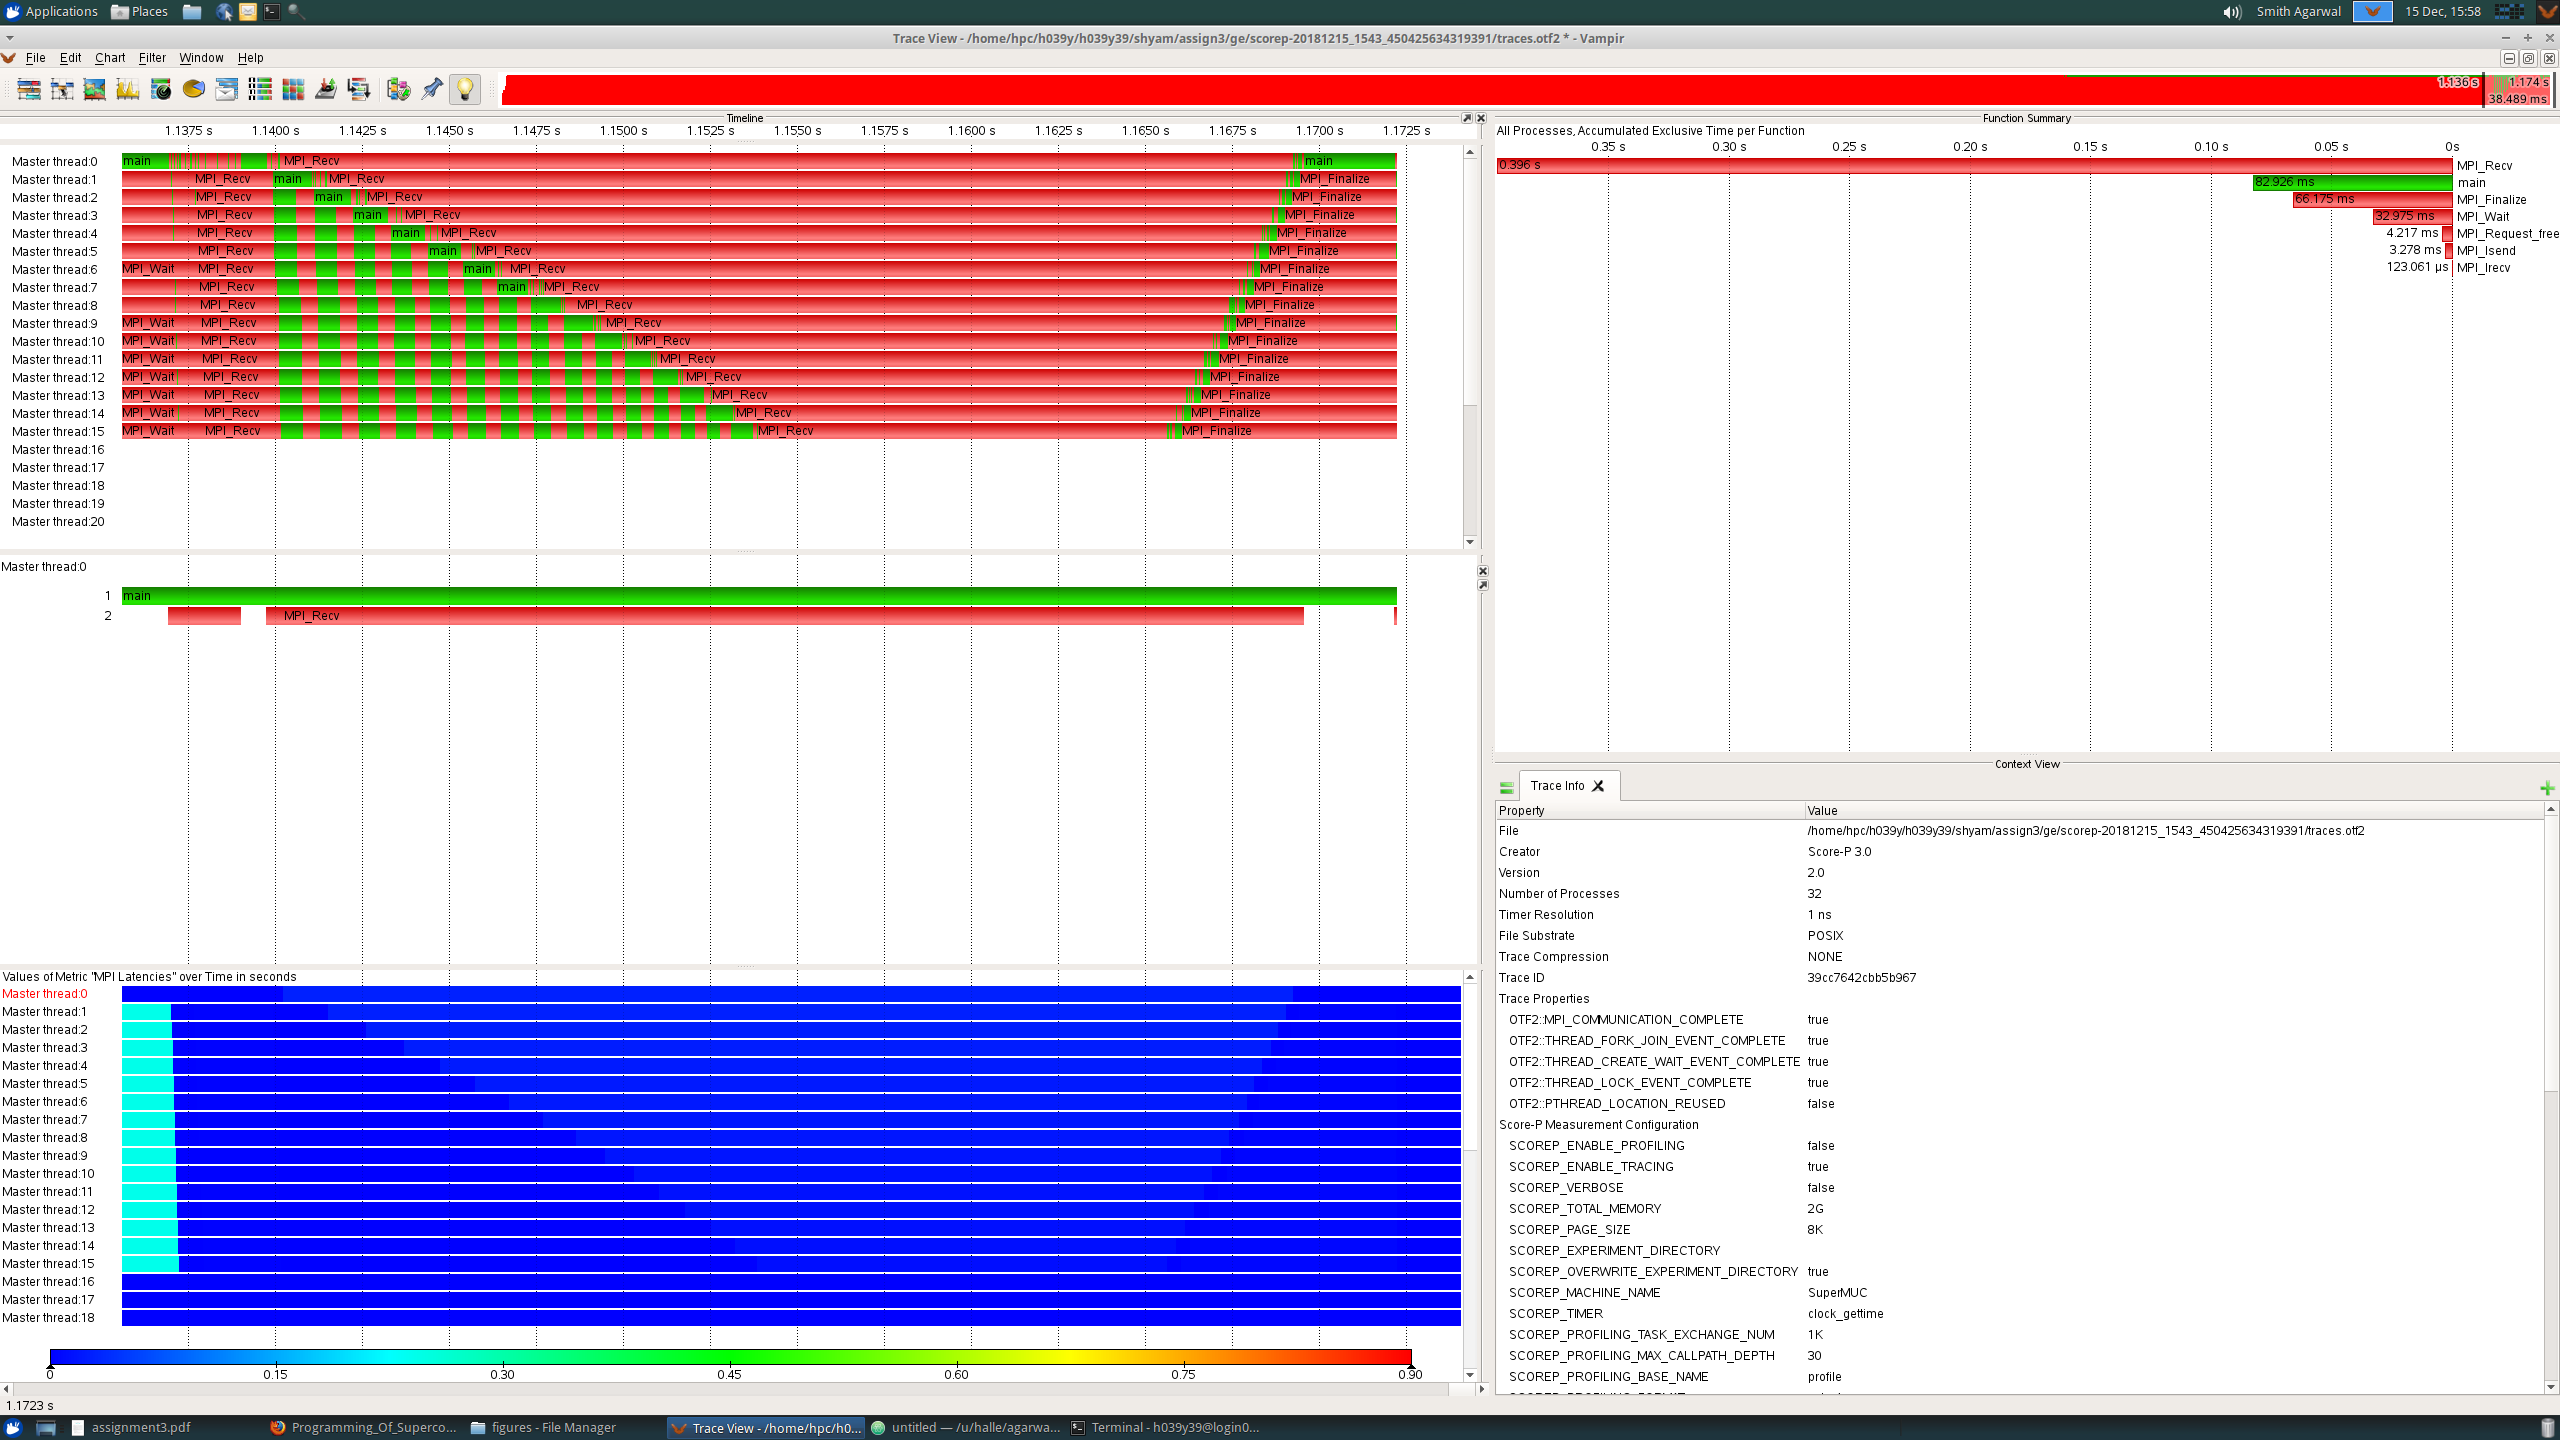
\includegraphics[scale = 0.16]{sb_nonblock_3.png}
\captionsetup{labelformat=empty}
\captionof{figure}{Figure : Vampir output for Point-to-point Sandy Bridge} 
\vspace{20mm}

\item \textbf{Was a speedup observed versus the baseline for the Sandy Bridge and Haswell nodes?} 

\vspace{5mm}
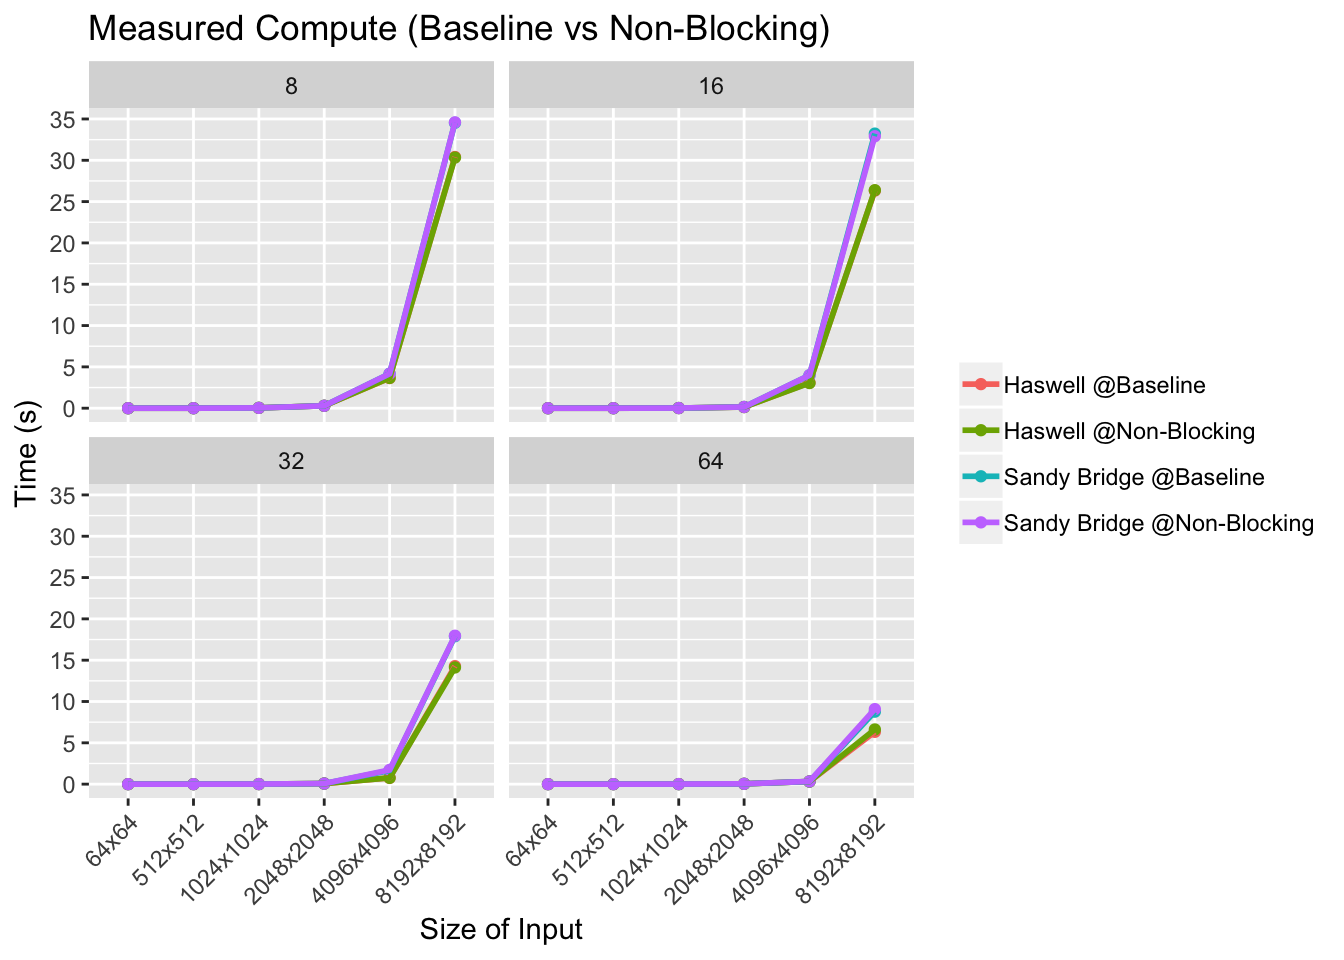
\includegraphics[scale = 0.18]{P2PBaseline_Measured-Compute_Processes.png}
%\captionof{figure}{example code for adding pic} 
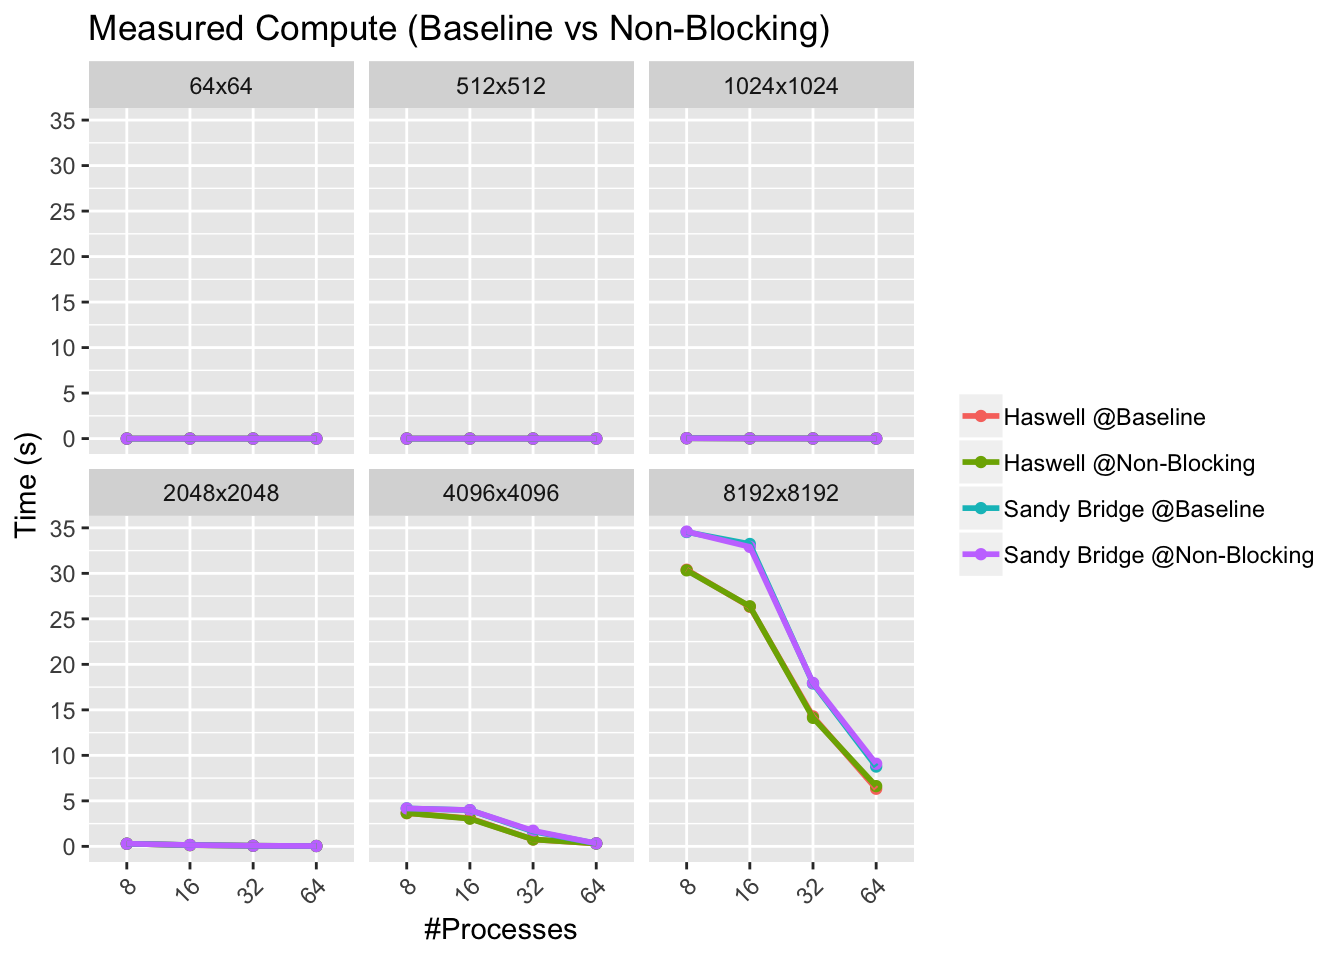
\includegraphics[scale = 0.18]{P2PBaseline_Measured-Compute_InputSize.png}
%\captionof{figure}{example code for adding pic} 
\vspace{5mm}
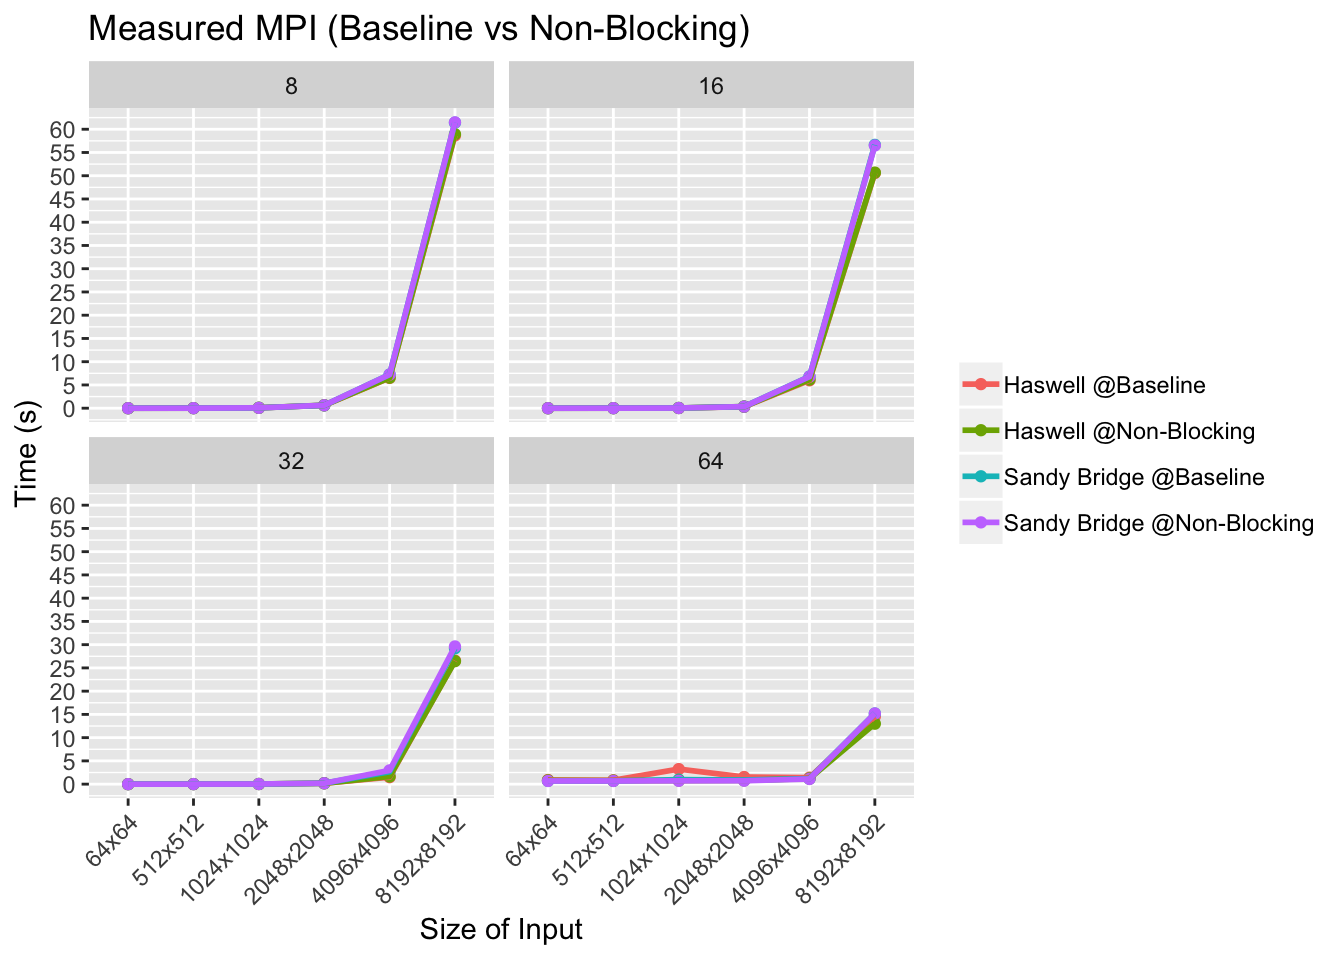
\includegraphics[scale = 0.18]{P2PBaseline_Measured-MPI_Processes.png}
%\captionof{figure}{example code for adding pic} 
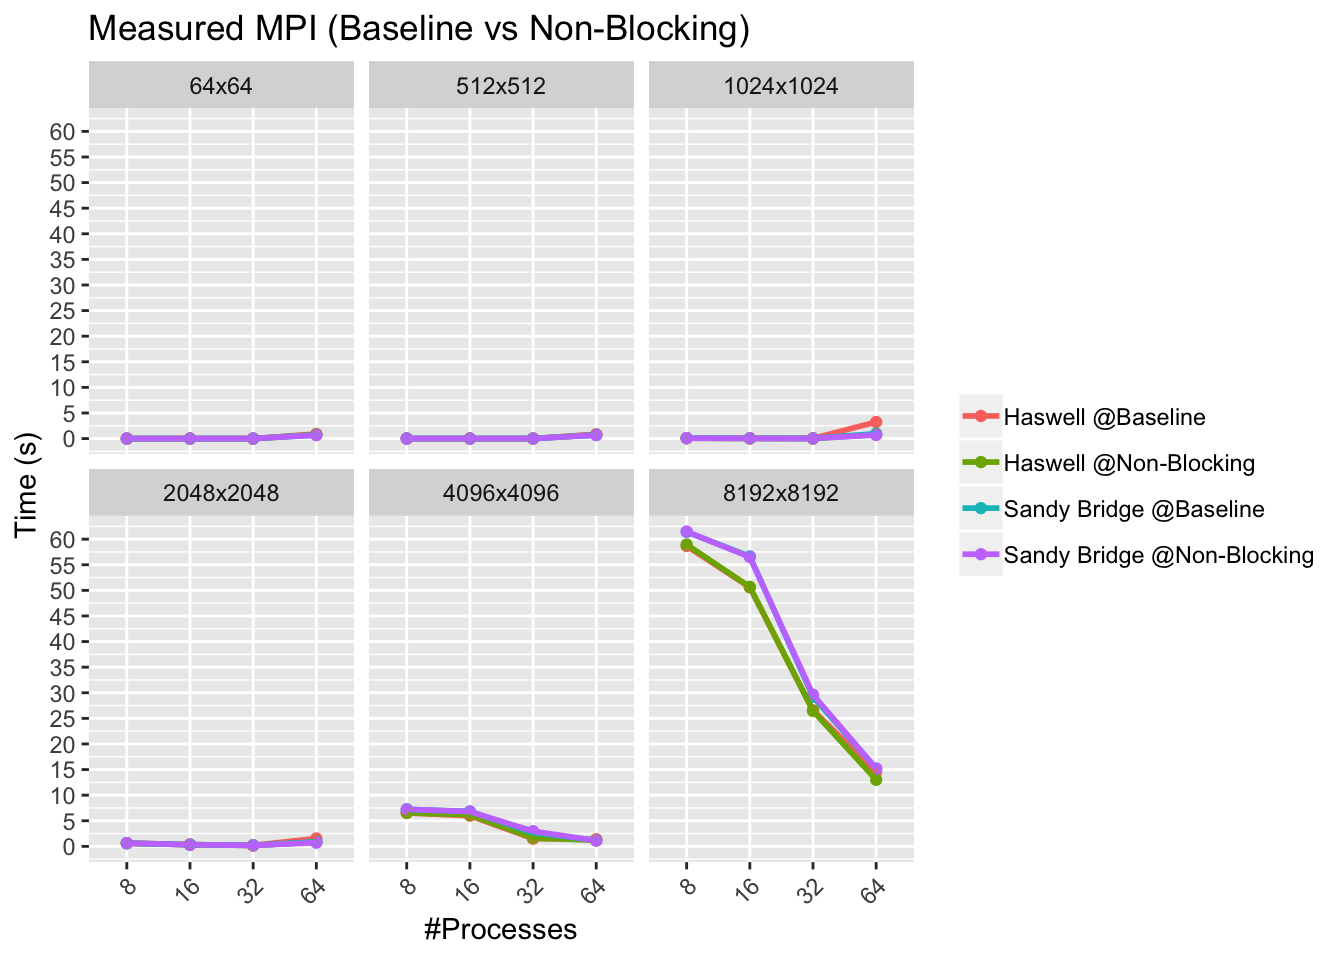
\includegraphics[scale = 0.18]{P2PBaseline_Measured-MPI_InputSize.png}
%\captionof{figure}{example code for adding pic} 
\vspace{5mm}
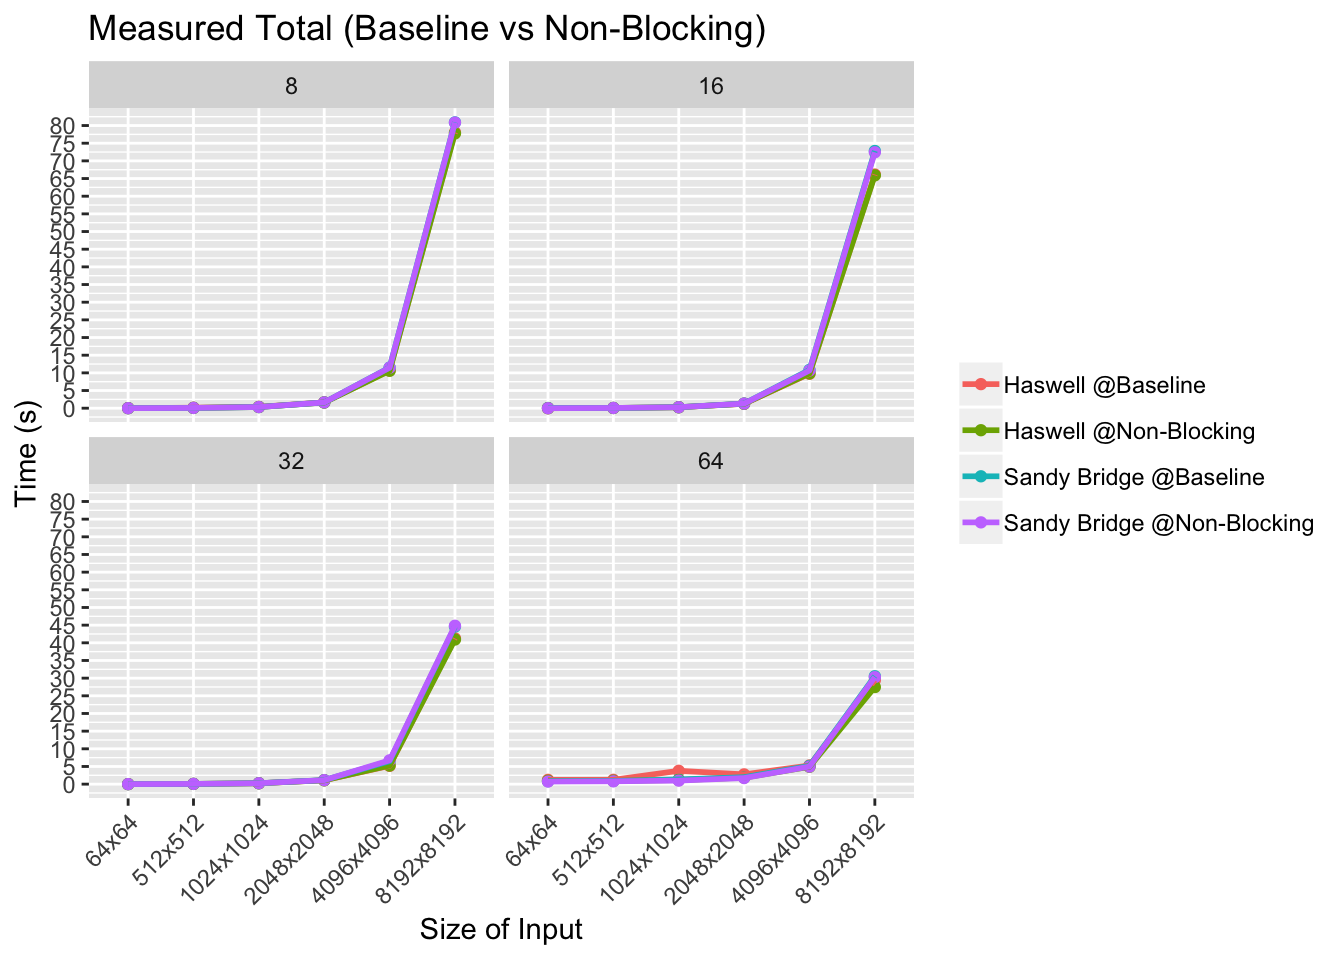
\includegraphics[scale = 0.18]{P2PBaseline_Measured-Total_Processes.png}
%\captionof{figure}{example code for adding pic} 
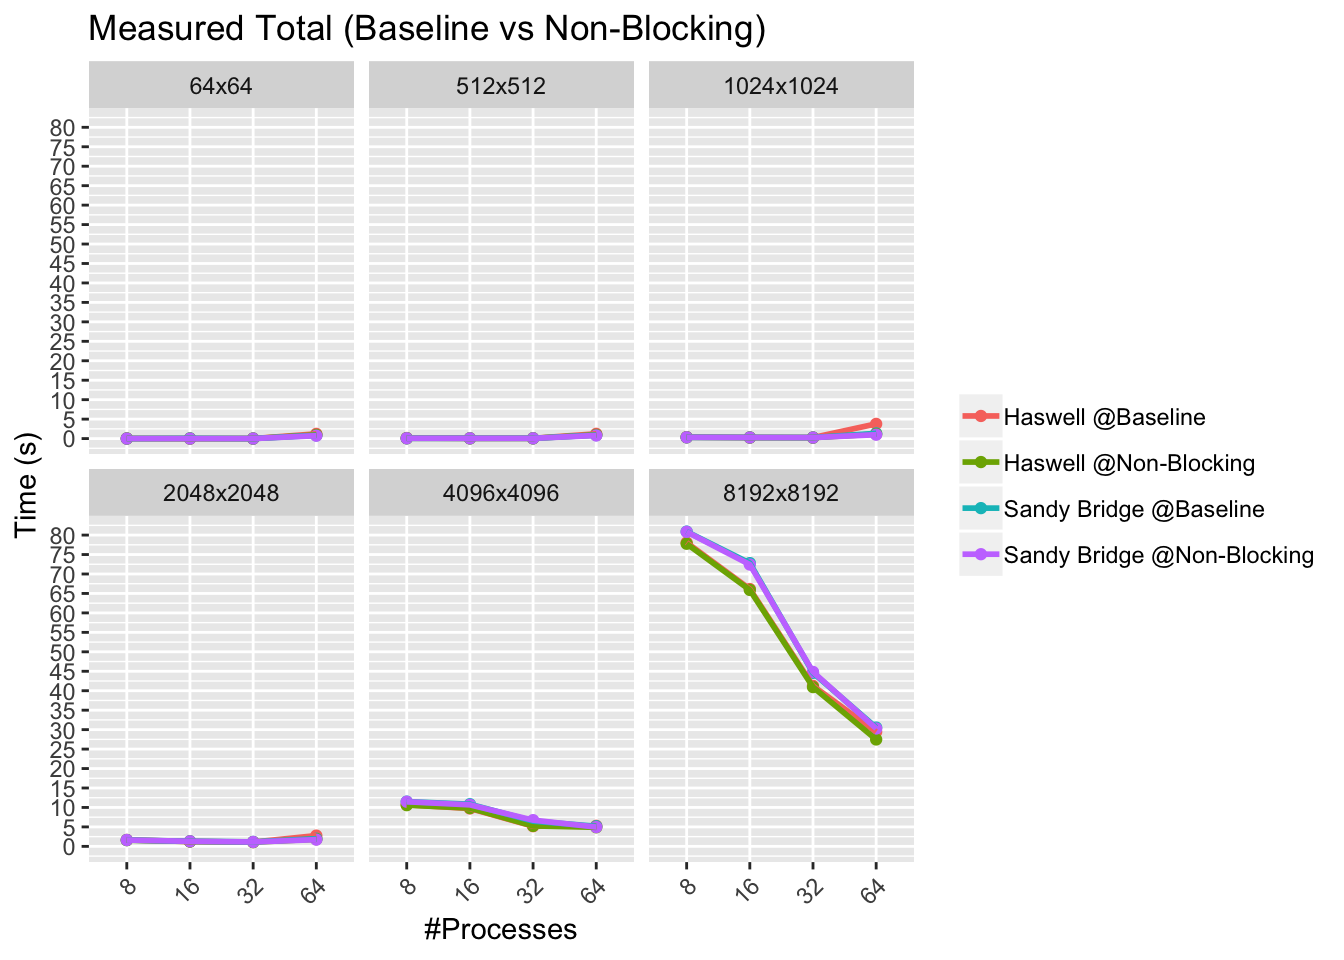
\includegraphics[scale = 0.18]{P2PBaseline_Measured-Total_InputSize.png}
%\captionof{figure}{example code for adding pic} 

Speedup is defined as \verb!time(baseline)! / \verb!time(non-blocking)! . From the plots, we observe than the non-blocking point-to-point communication performed slightly better than the baseline, however speedup was little due to lack of overlap of communication and computation. As we proceed with computation, more processes remain idle because each process requires the data computed by previous loop.

\end{enumerate}

\section{MPI One-Sided Communication}

\subsection{Required submission files}

\begin{enumerate}
\item \textbf{The updated gauss.c file.} 

Refer gauss\_oneside.c file from code scripts of Task 5.1  

\item \textbf{The new performance plots and the description in the report.} 

The various performance plots for MPI One-Sided communication are:\\
\\
\vspace{10mm}
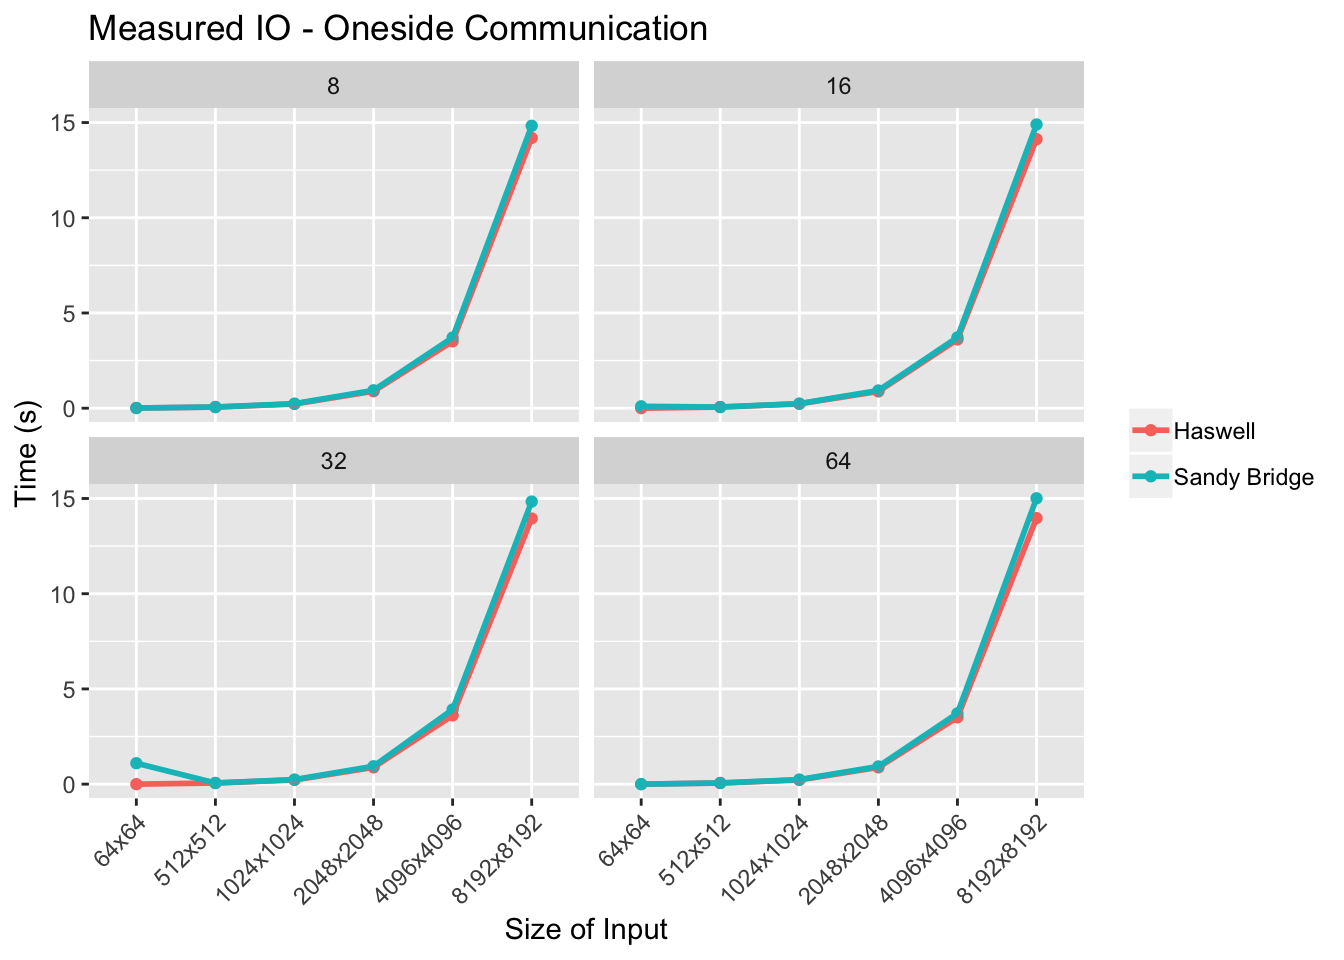
\includegraphics[scale = 0.18]{OS_Measured-IO_Processes.png}
%\captionof{figure}{example code for adding pic} 
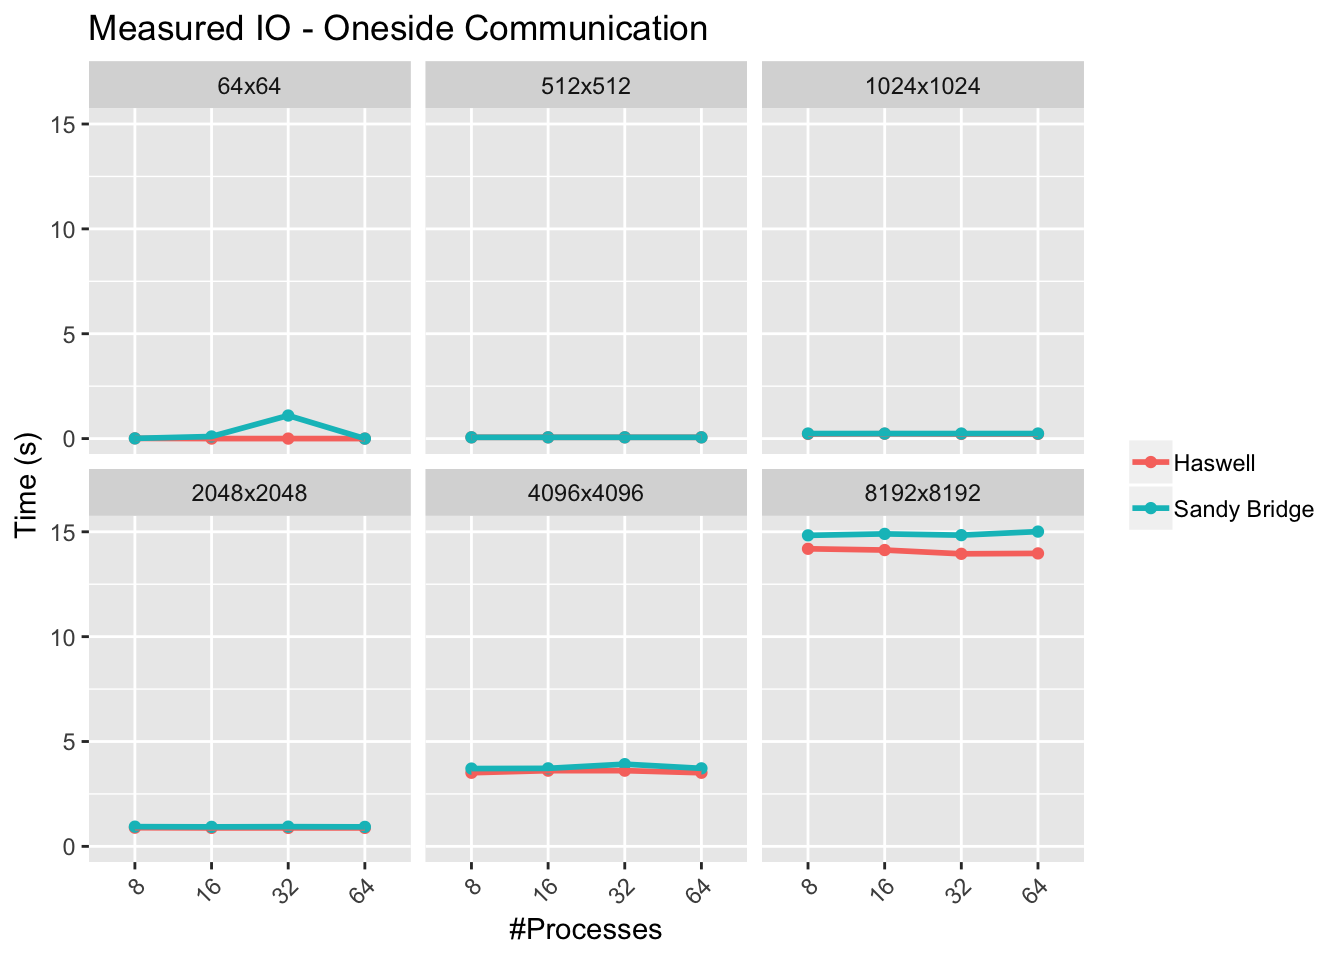
\includegraphics[scale = 0.18]{OS_Measured-IO_InputSize.png}
%\captionof{figure}{example code for adding pic} 
\vspace{10mm}
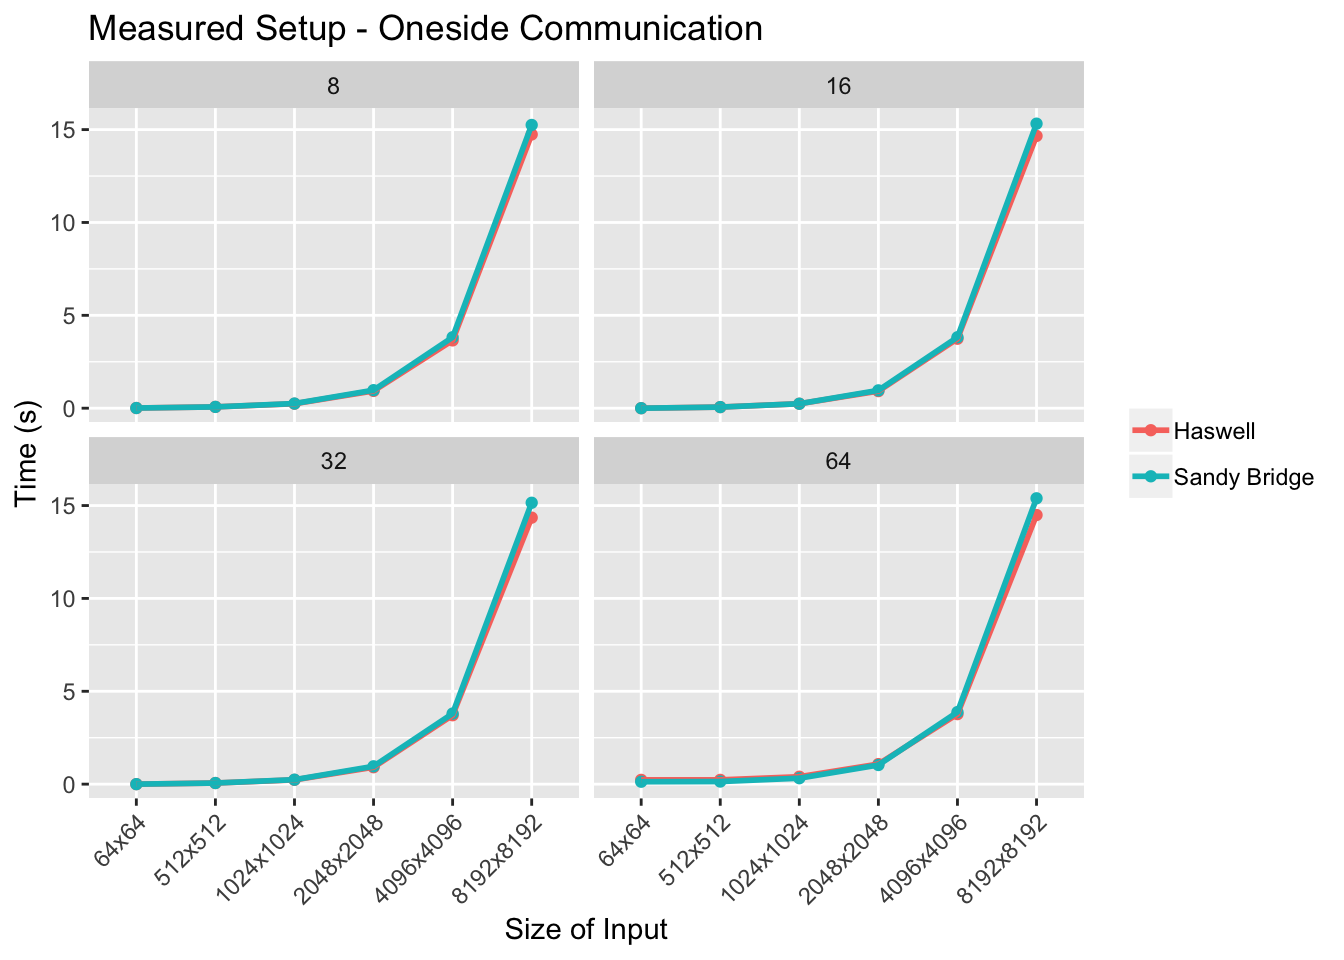
\includegraphics[scale = 0.18]{OS_Measured-Setup_Processes.png}
%\captionof{figure}{example code for adding pic} 
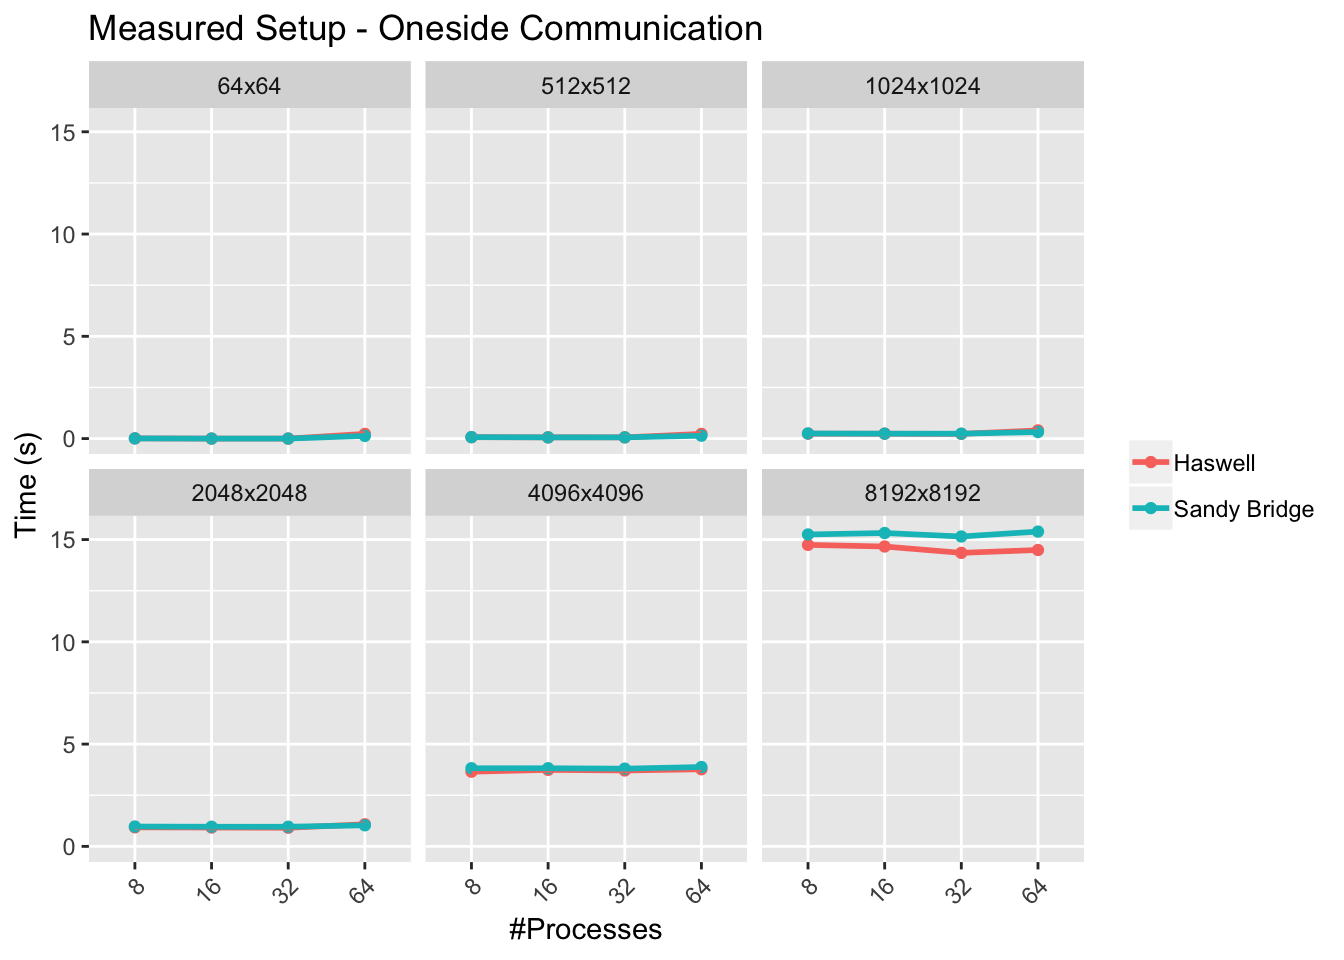
\includegraphics[scale = 0.18]{OS_Measured-Setup_InputSize.png}
%\captionof{figure}{example code for adding pic} 
\vspace{100mm}
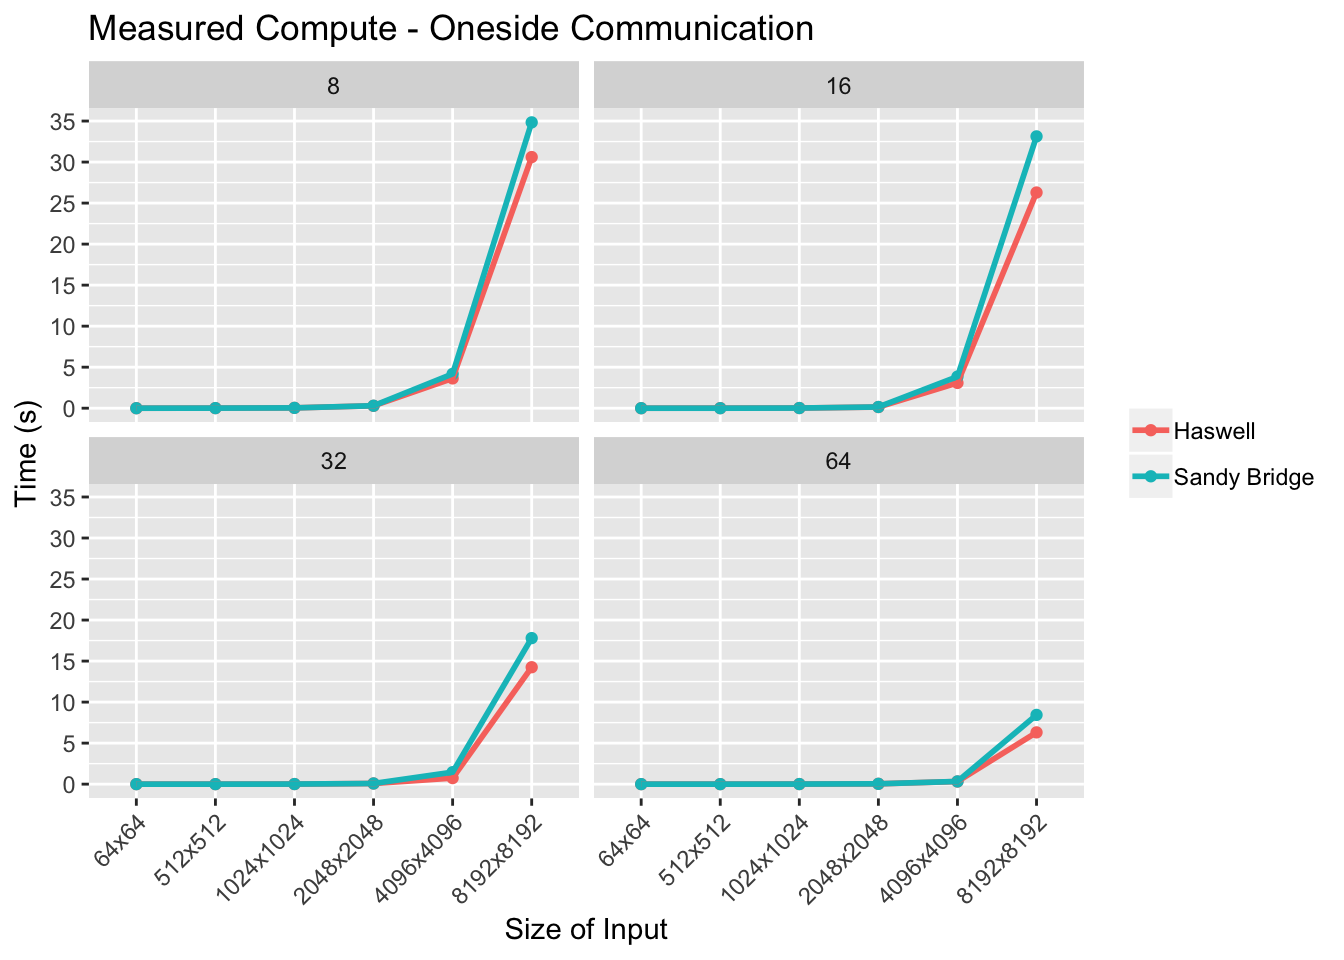
\includegraphics[scale = 0.18]{OS_Measured-Compute_Processes.png}
%\captionof{figure}{example code for adding pic} 
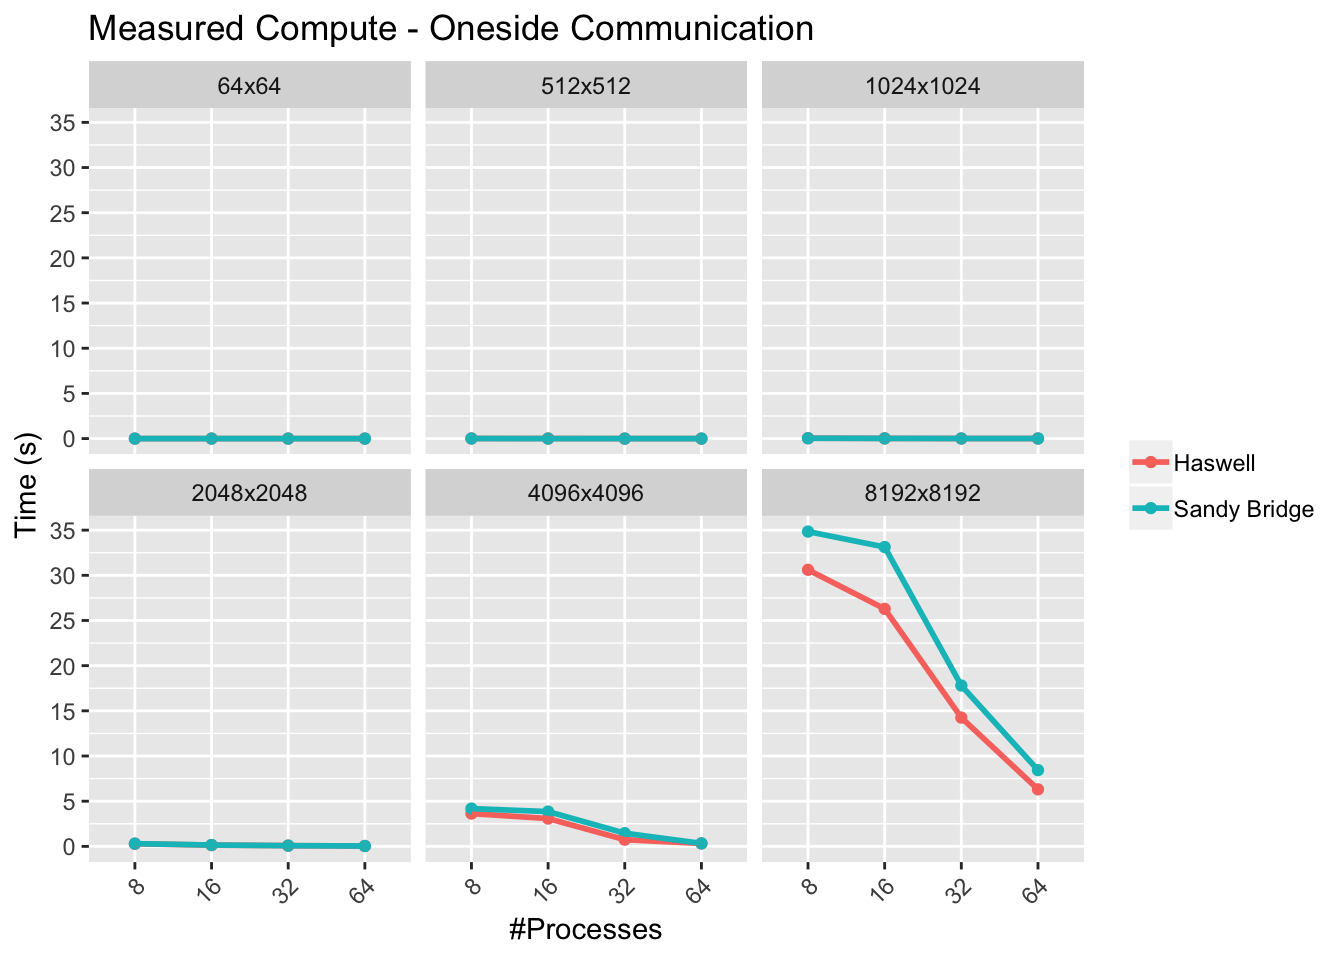
\includegraphics[scale = 0.18]{OS_Measured-Compute_InputSize.png}
%\captionof{figure}{example code for adding pic} 
\vspace{10mm}
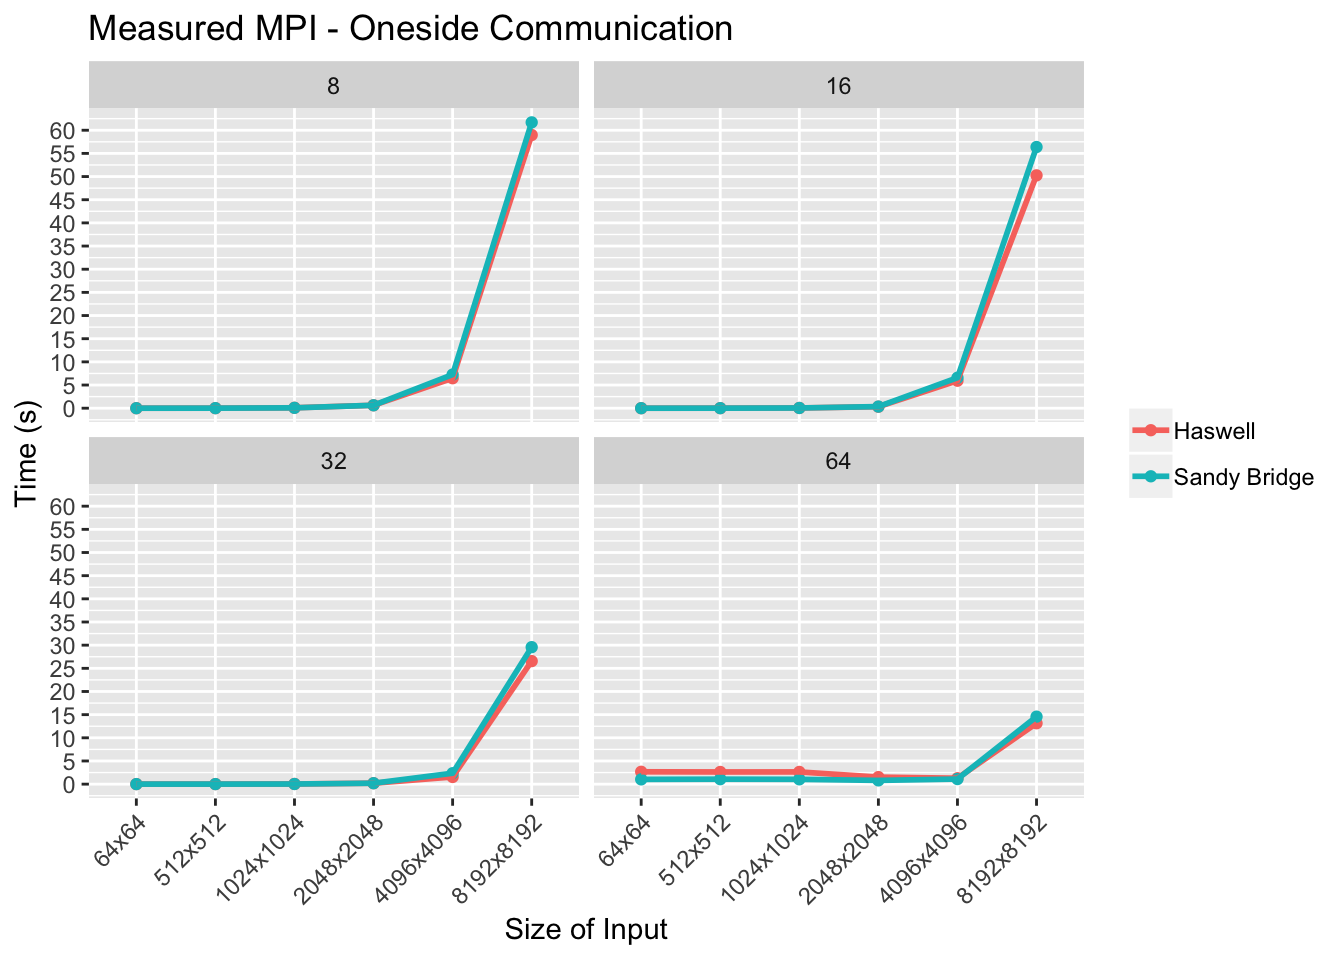
\includegraphics[scale = 0.18]{OS_Measured-MPI_Processes.png}
%\captionof{figure}{example code for adding pic} 
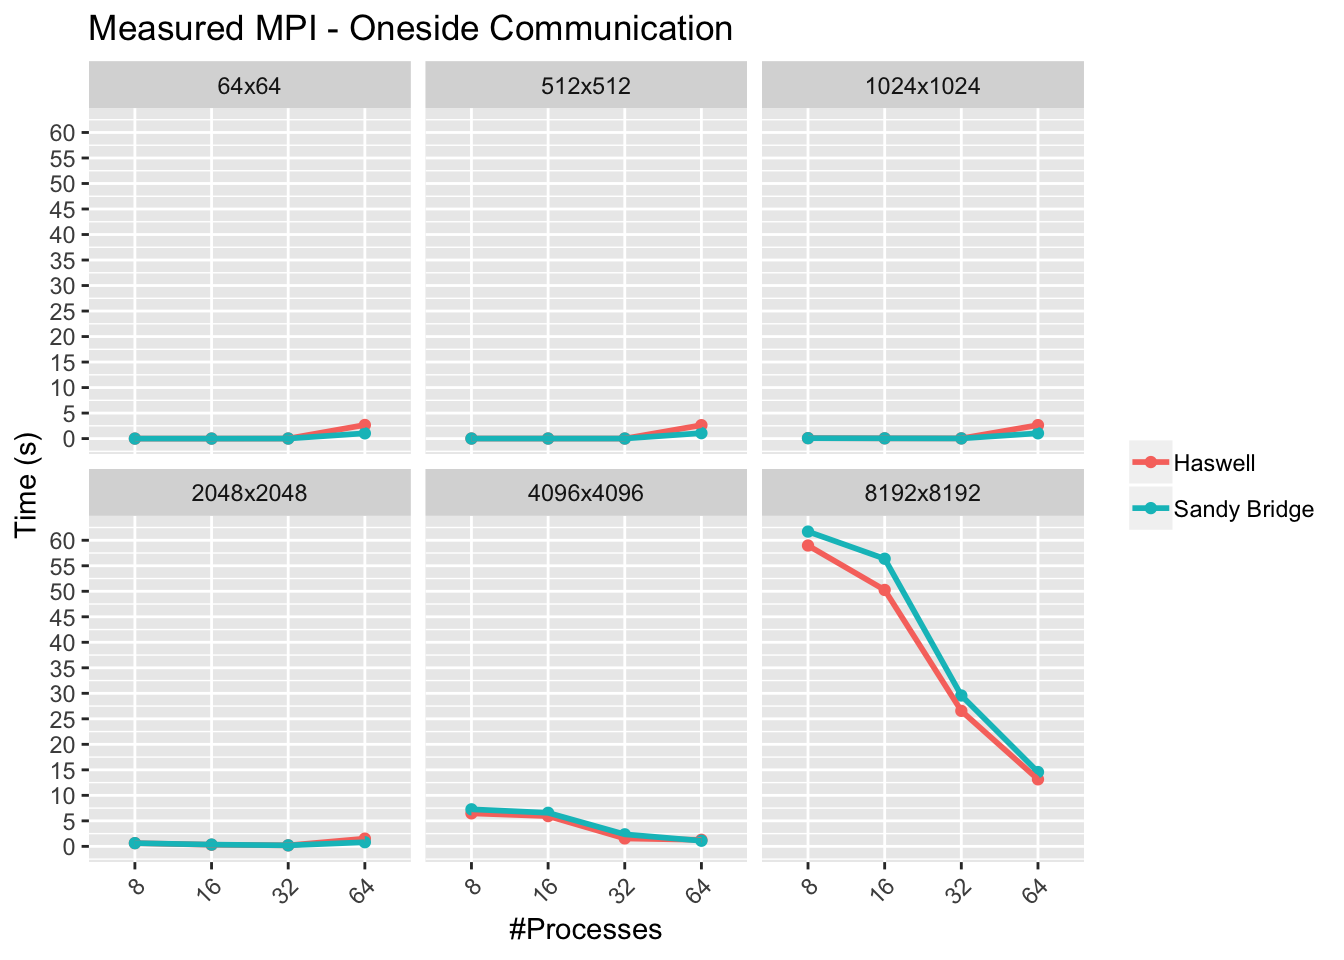
\includegraphics[scale = 0.18]{OS_Measured-MPI_InputSize.png}
%\captionof{figure}{example code for adding pic} 
\vspace{5mm}
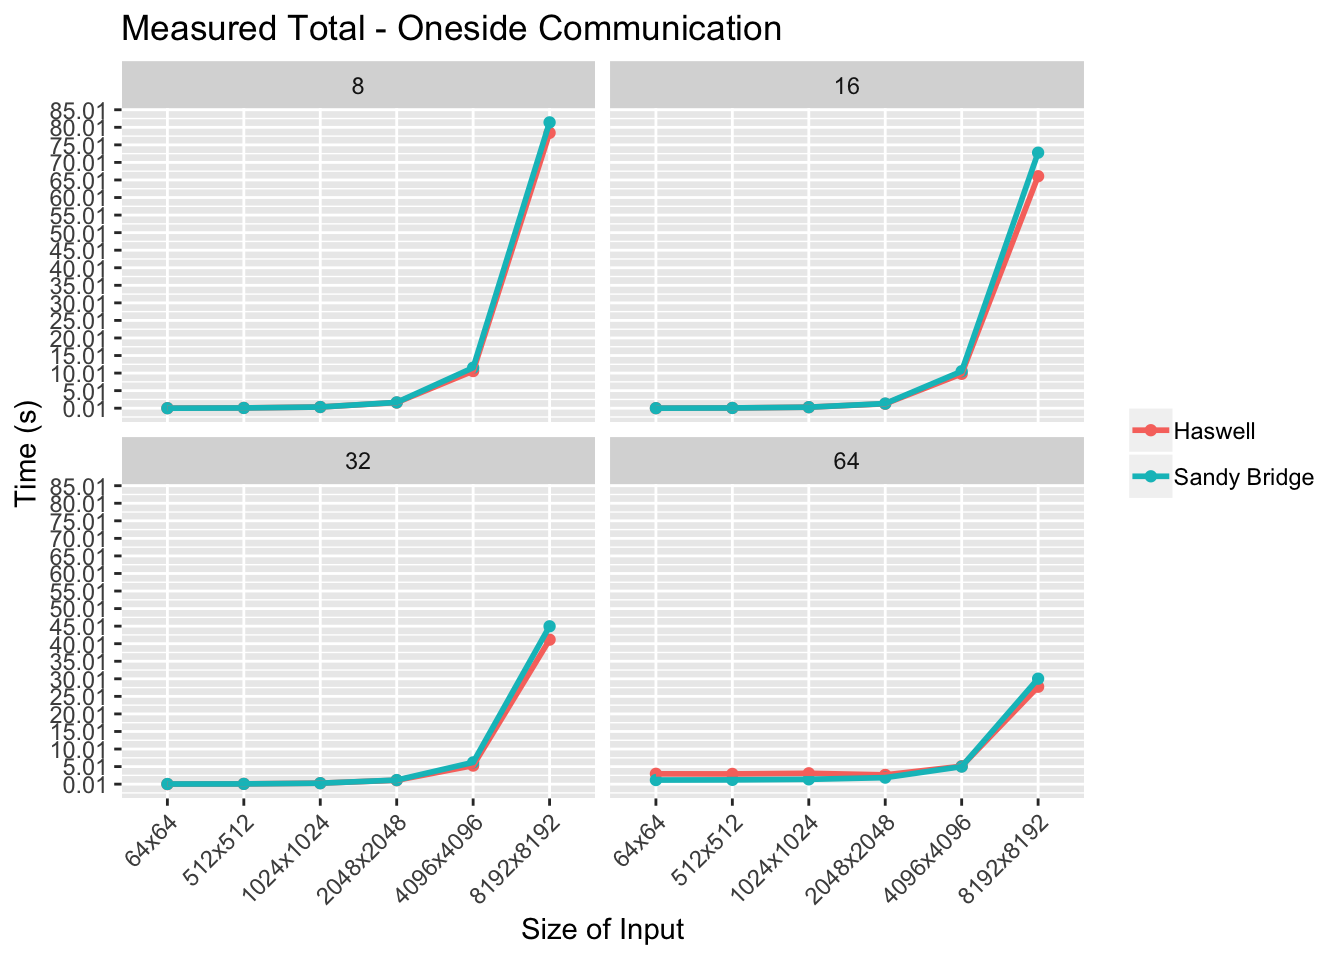
\includegraphics[scale = 0.18]{OS_Measured-Total_Processes.png}
%\captionof{figure}{example code for adding pic} 
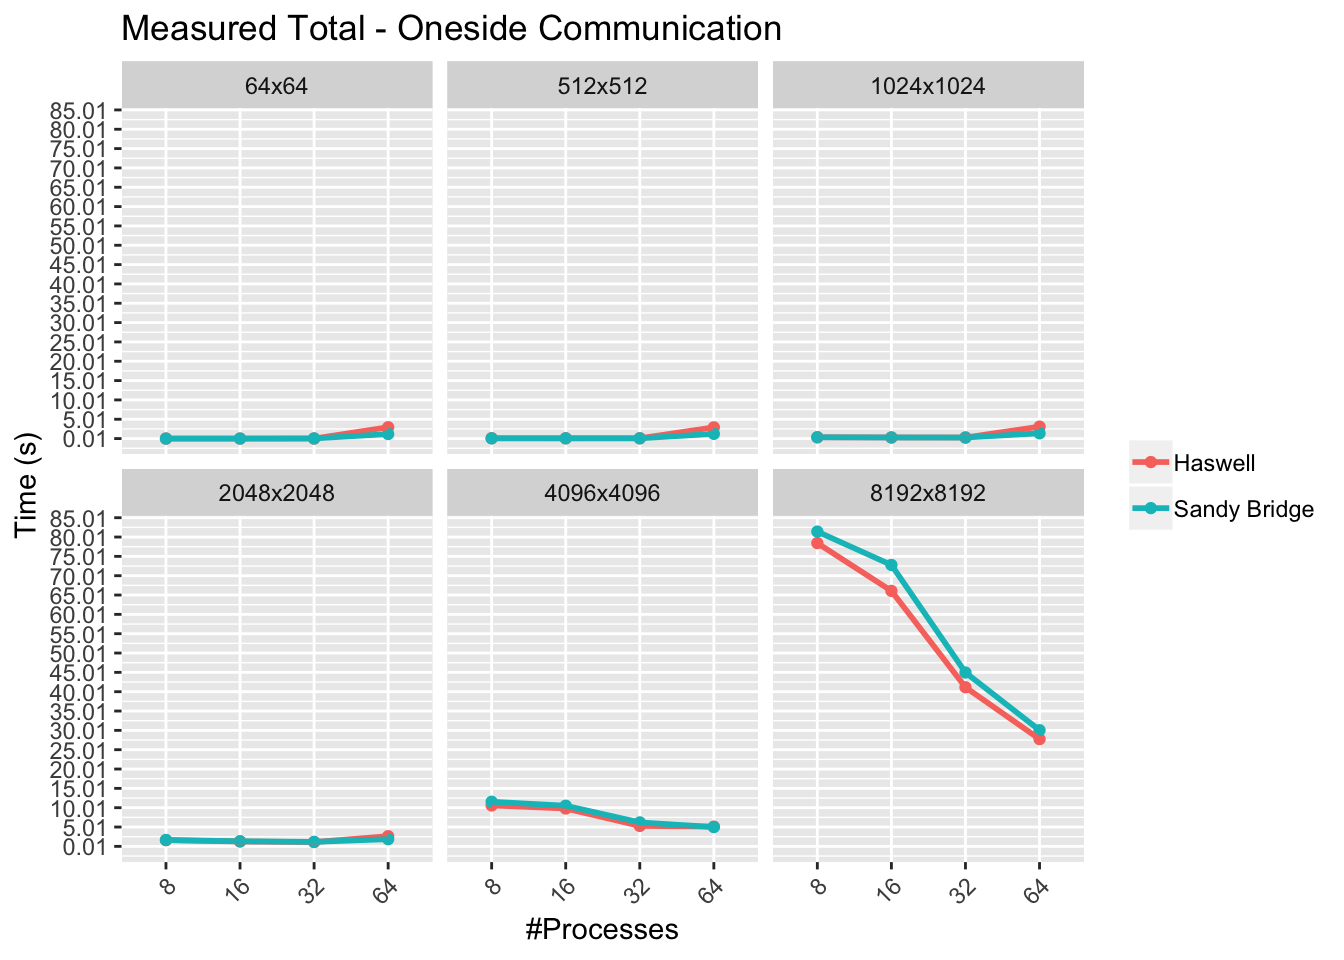
\includegraphics[scale = 0.18]{OS_Measured-Total_InputSize.png}
%\captionof{figure}{example code for adding pic} 
\end{enumerate} 

\subsection{Questions}

\begin{enumerate}
\item\textbf{Which one-sided operations were used? Justify your choice.}

MPI two-sided communication might sometimes cause a delay in sending data, since the sender has to wait for the receiver to be ready to receive the data before it can send it. 

To overcome this drawback, the MPI 2 standard introduced Remote Memory Access RMA, also called 'One-Sided communication' because it requires only one process to transfer data. Basically, the idea of one-sided communication models is to decouple data movement with process synchronization.

We have used Post-Start-Wait-Complete methodology	and following one-sided operations were used :-
\begin{enumerate}
  \item \textbf{MPI\_Win\_create :} it is called by all processes to create a window of shared memory, the window specifies all process memory which is available for remote operations. Each process then initializes its portion of the memory window allowing remote processes read/write access to the pre-defined memory. 
  \item \textbf{MPI\_Win\_allocate :} MPI allocates local memory and returns a pointer to it
  \item \textbf{MPI\_Win\_start :} Starts an RMA access epoch for MPI
  \item \textbf{MPI\_Put :} writes data from local memory into a memory window on a remote process 
  \item \textbf{MPI\_Get :} reads data from a memory window on a remote process into local memory
  \item \textbf{MPI\_Win\_fence :} helps in collective synchronization of all processes. 
  \item \textbf{MPI\_Win\_free :} Terminates the memory window and deallocates window object.
  \item \textbf{MPI\_Finalize :} Cleans up all MPI states and MPI environment. The parallel code ends here.

\end{enumerate} 

\vspace{10mm}

	
\item\textbf{Was communication and computation overlap achieved? Use Vampir.} 

Yes, communication and computation overlap was achieved and this can be observed from the below vampir plots. 

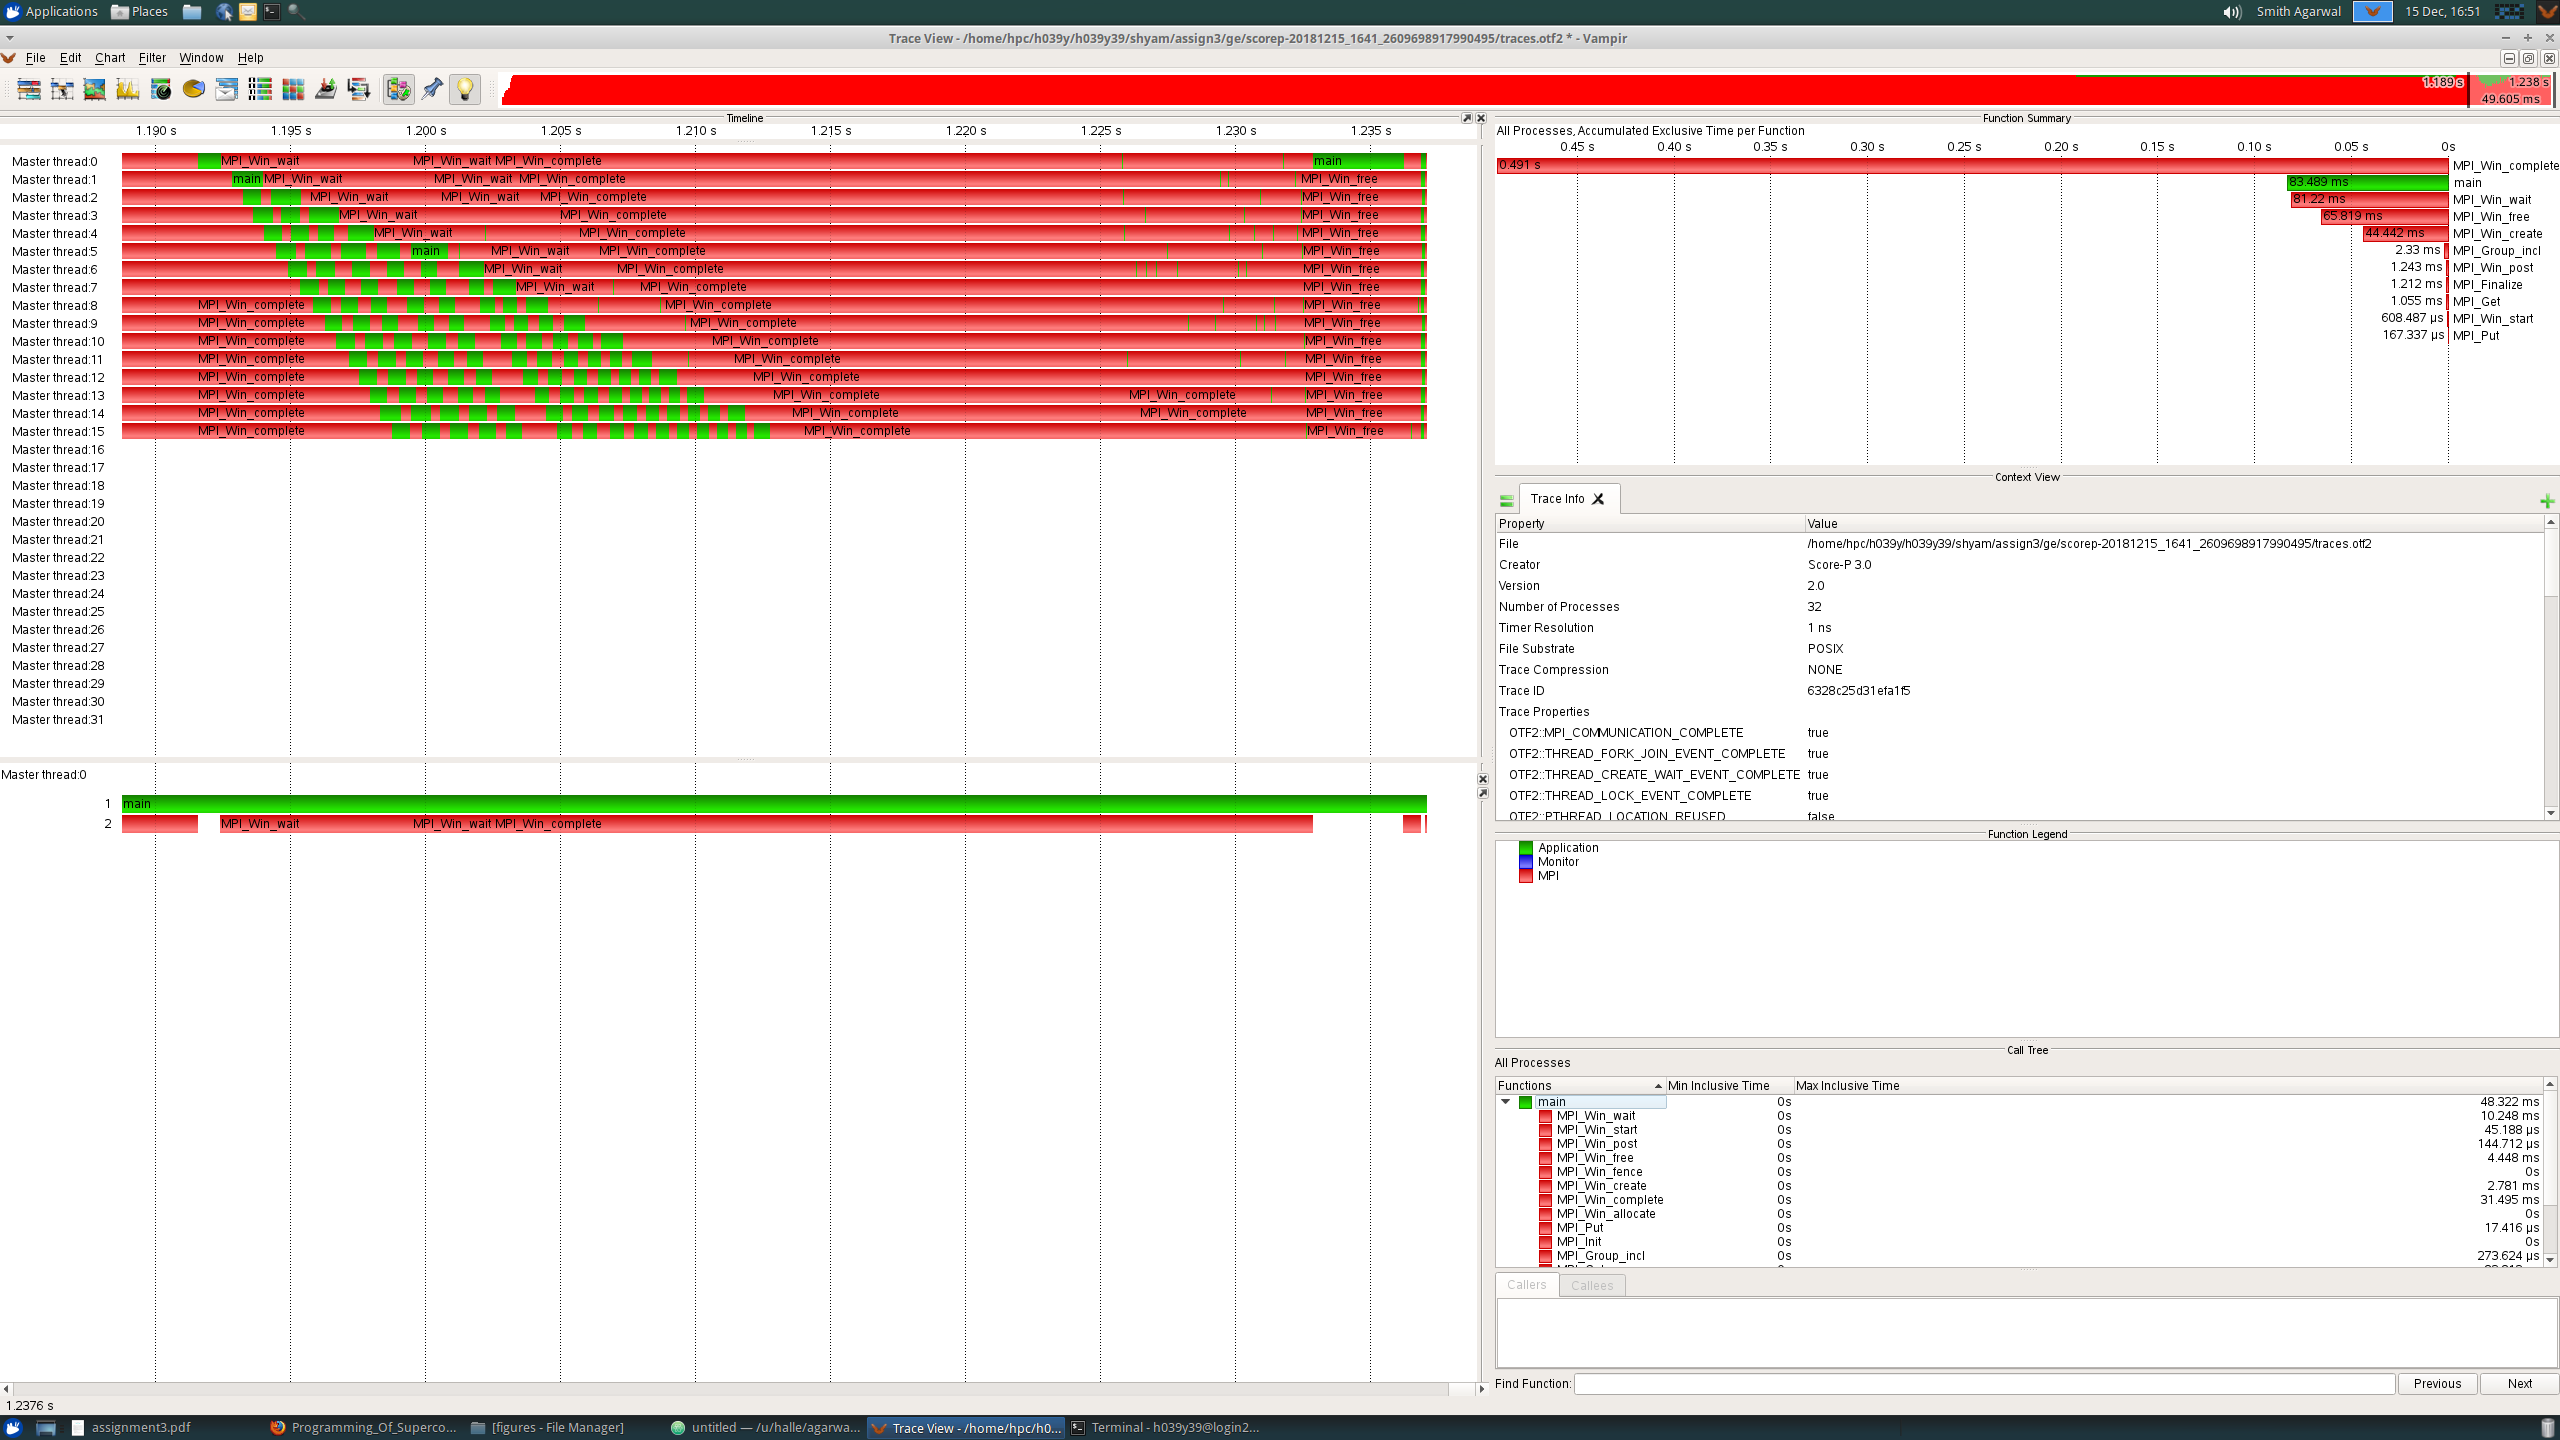
\includegraphics[scale = 0.16]{hw_oneside_3.png}
\captionsetup{labelformat=empty}
\captionof{figure}{Figure : Vampir output for One-sided Haswell} 

\vspace{10mm}
\hspace{7mm}
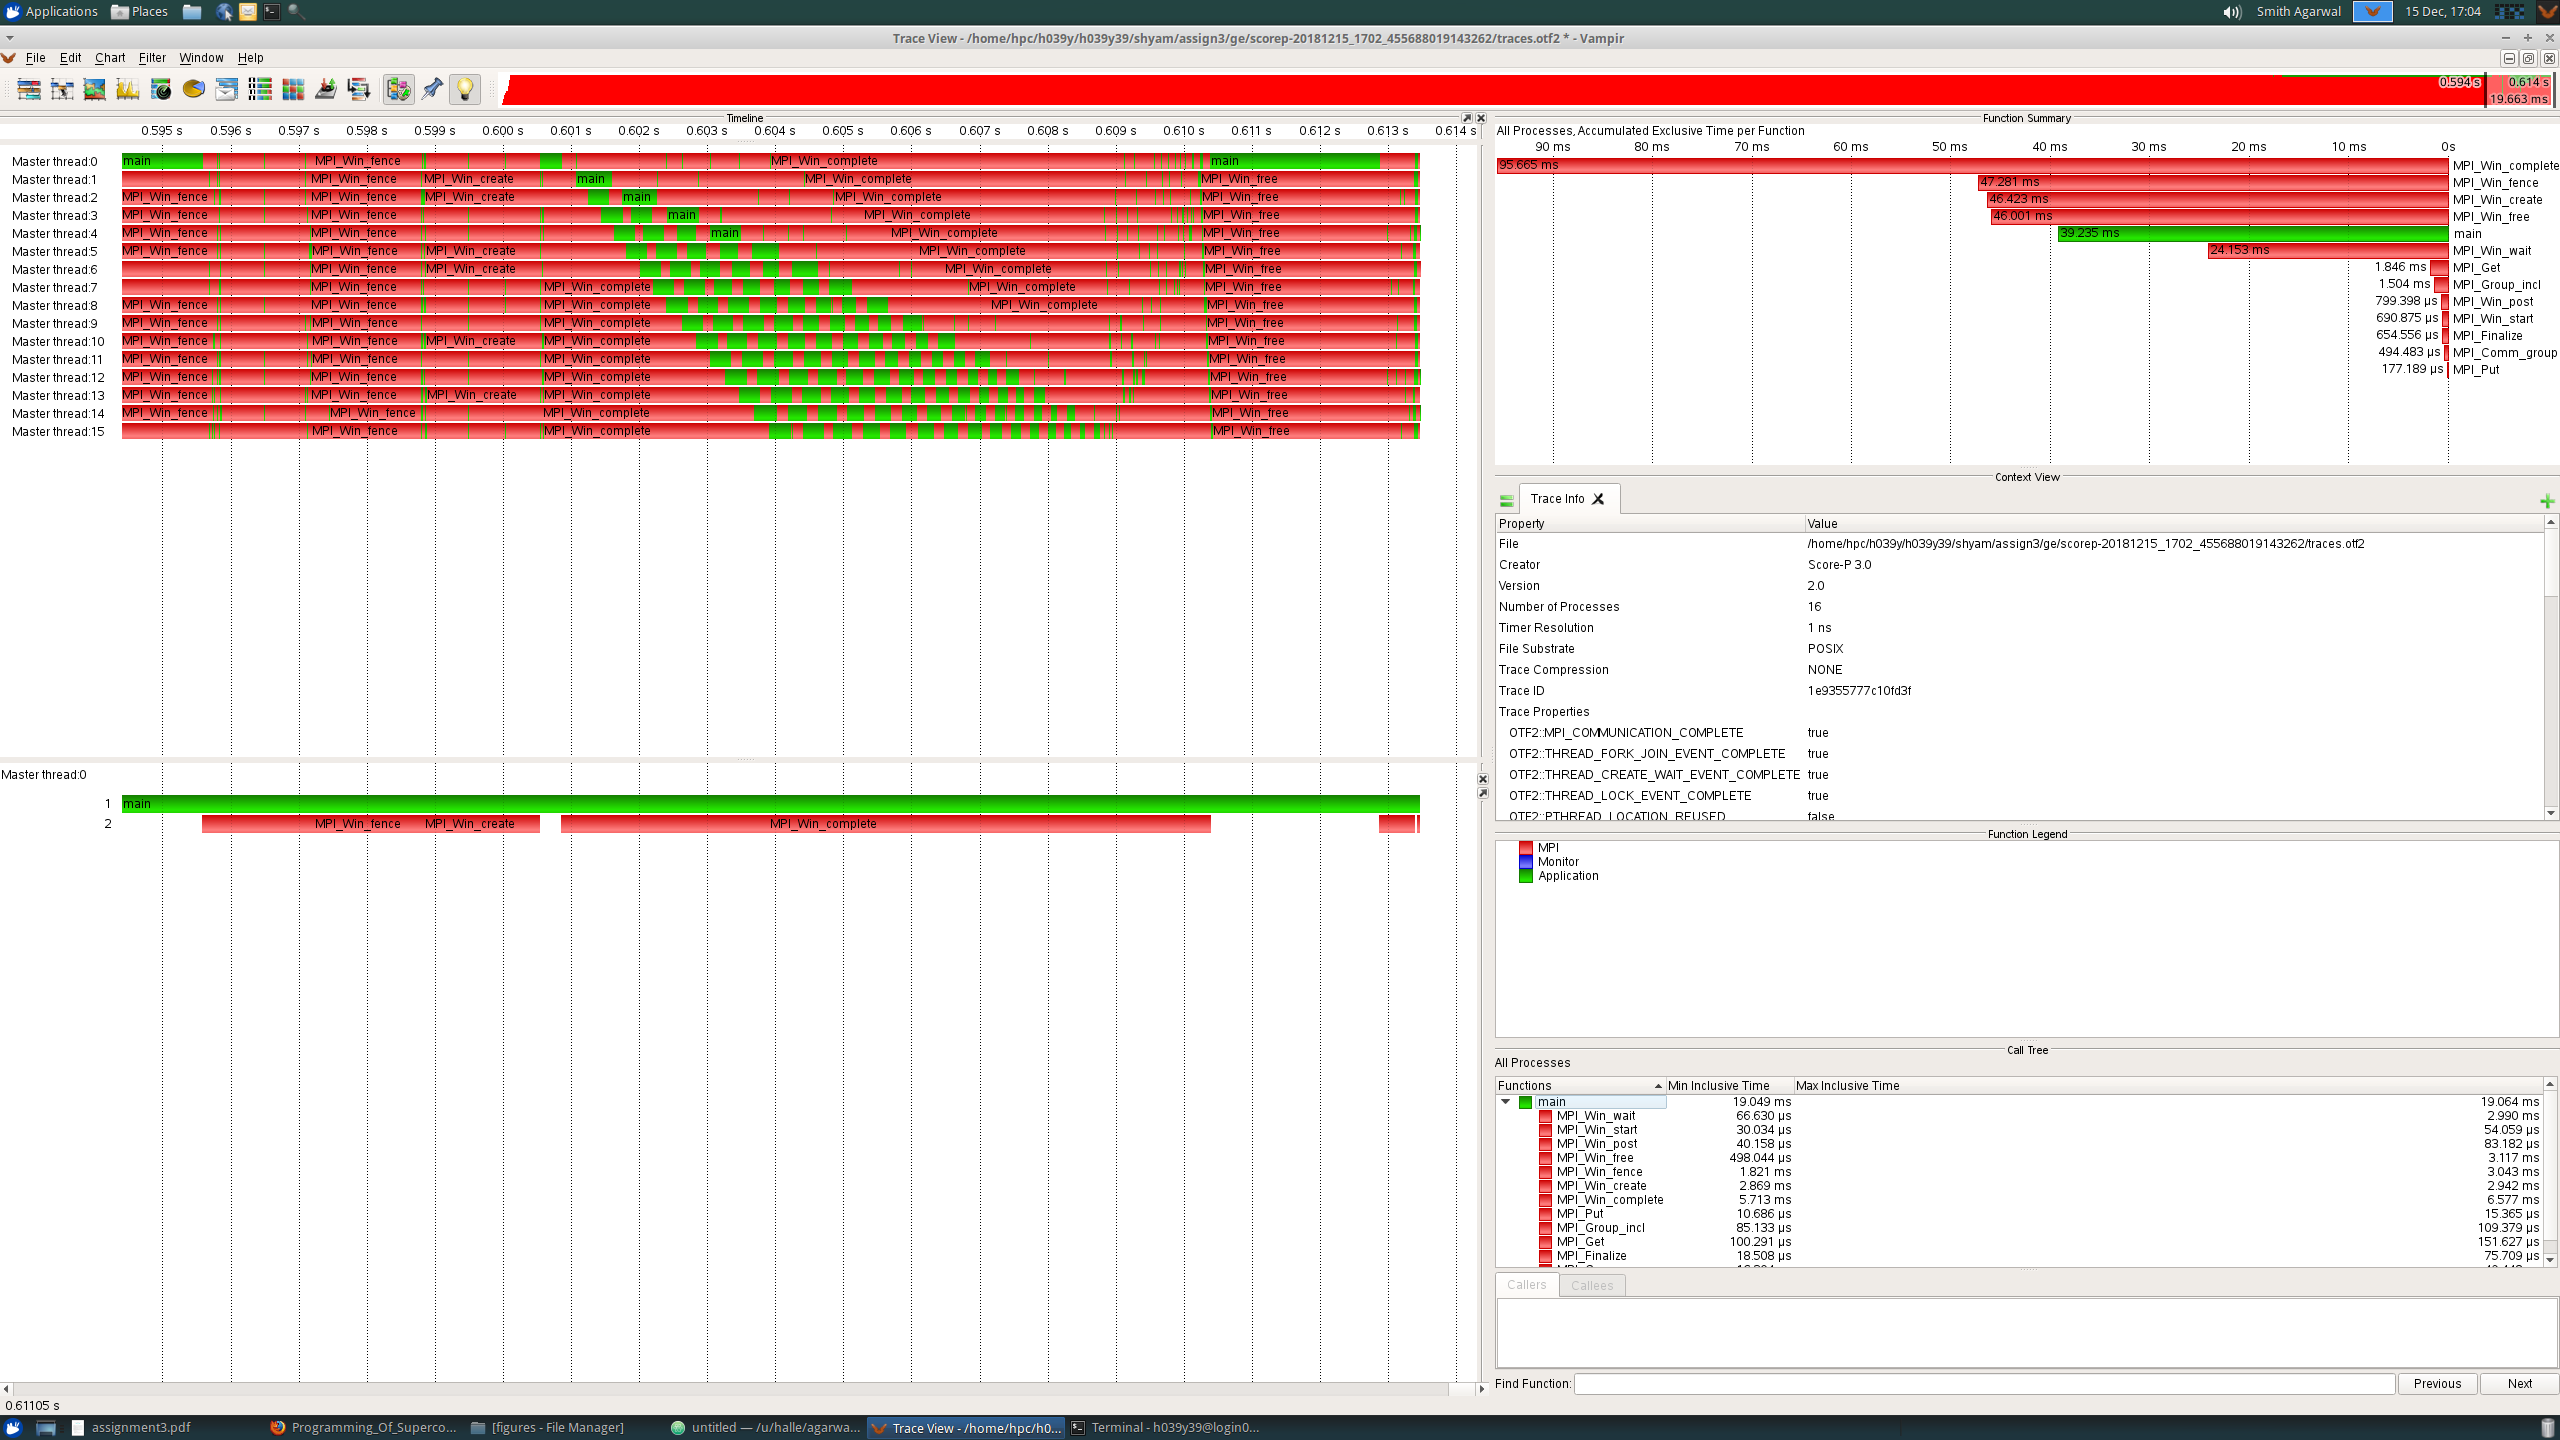
\includegraphics[scale = 0.16]{sb_oneside_2.png}
\captionsetup{labelformat=empty}
\captionof{figure}{Figure : Vampir output for One-sided Sandy Bridge}	


\item \textbf{Was a speedup observed versus the baseline for the Sandy Bridge and Haswell nodes?} \\

Speedup here is defined as \verb!time(baseline)! / \verb!time(one-sided)! . Both Sandy Bridge and Haswell nodes performed almost the same for One-sided communication with respect to baseline. From the plots, we observe that good overlap was achieved, but there was significant performance slow down.

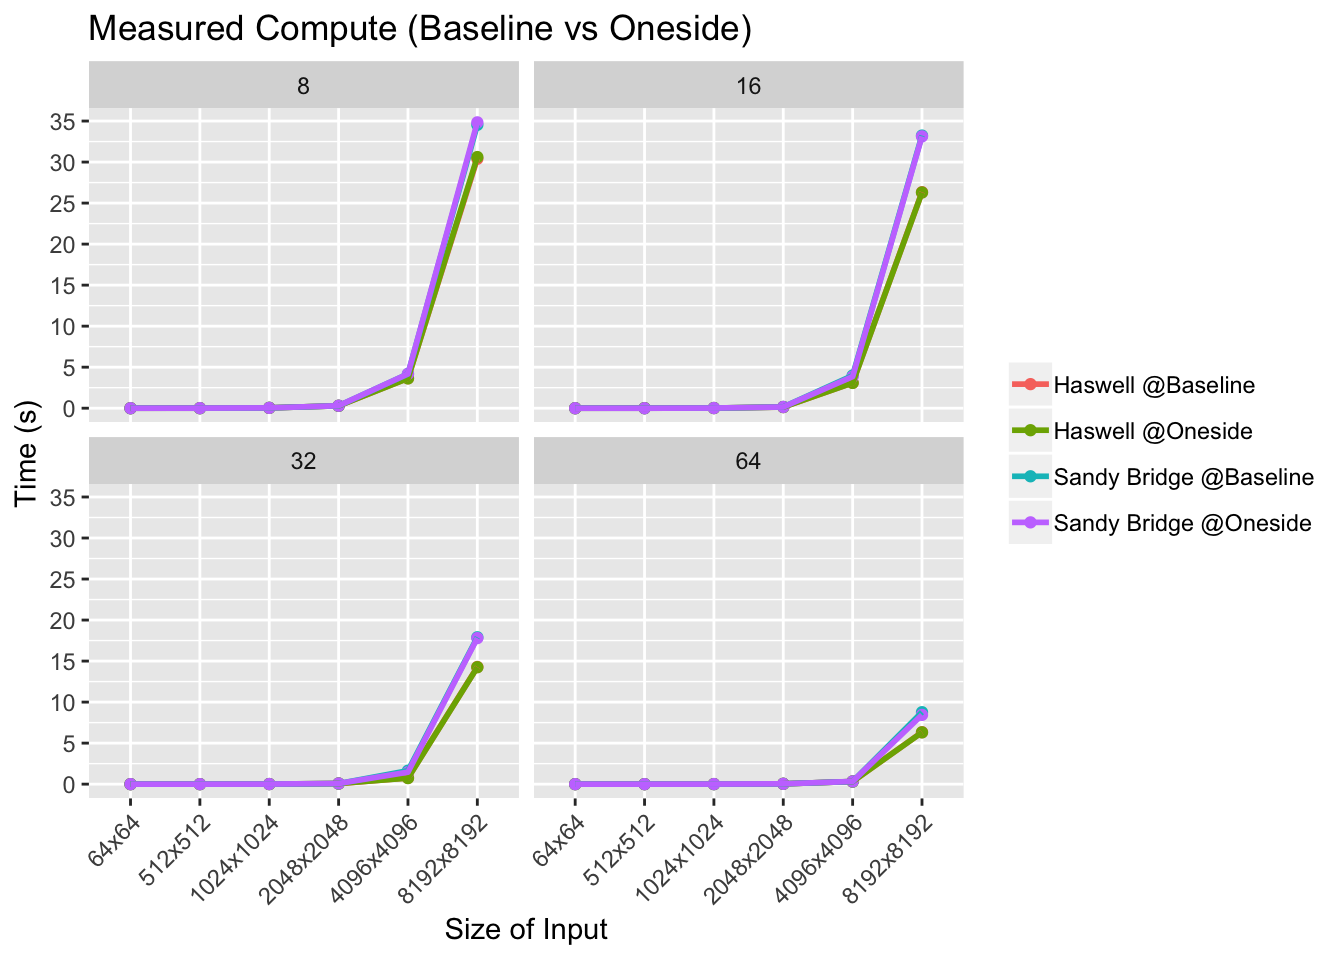
\includegraphics[scale = 0.18]{OSBaseline_Measured-Compute_Processes.png}
%\captionof{figure}{example code for adding pic} 
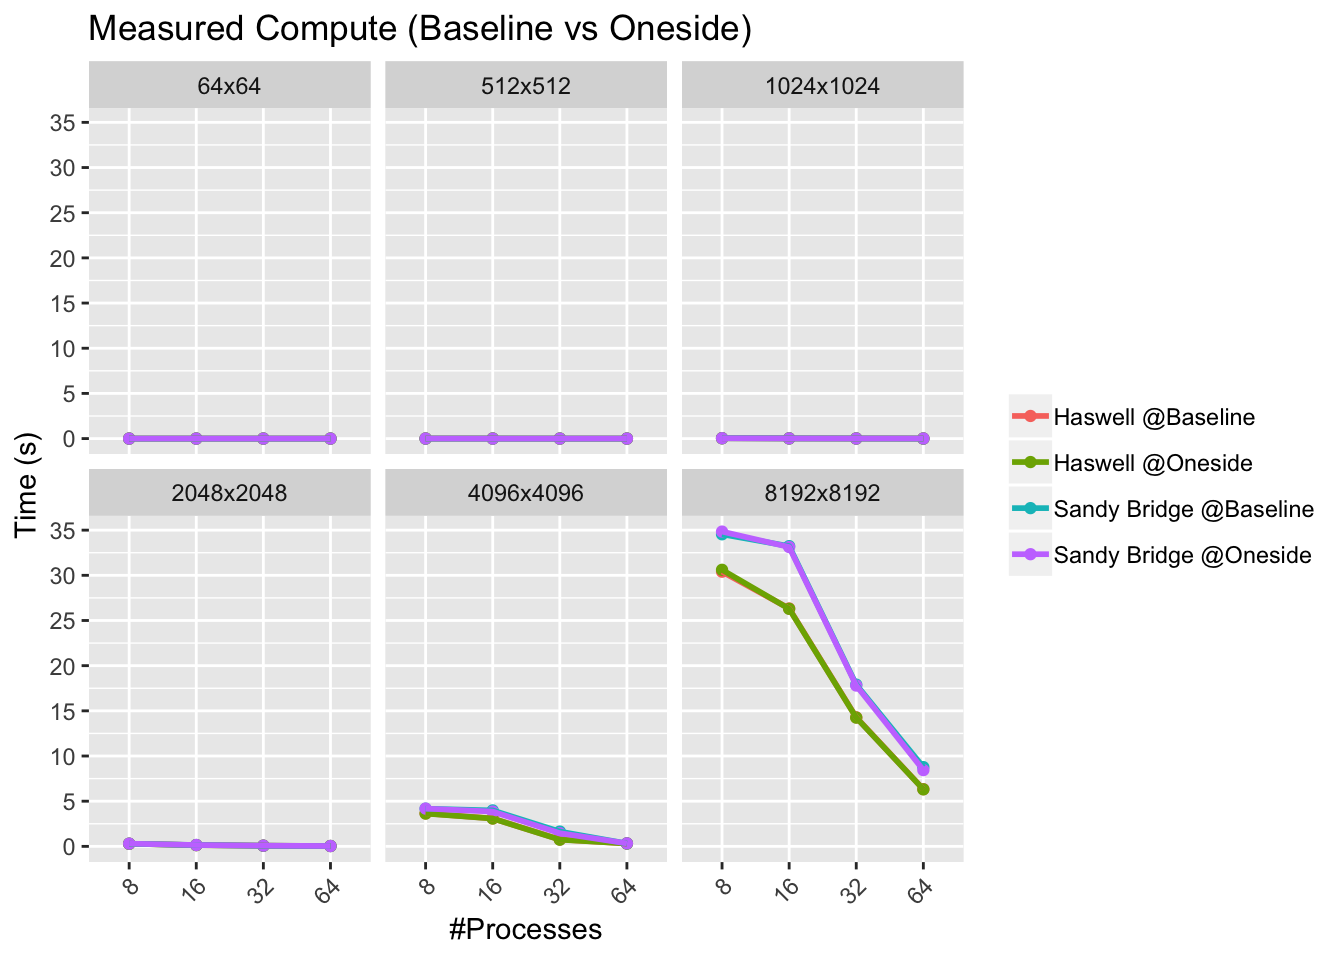
\includegraphics[scale = 0.18]{OSBaseline_Measured-Compute_InputSize.png}
%\captionof{figure}{example code for adding pic} 
\vspace{10mm}
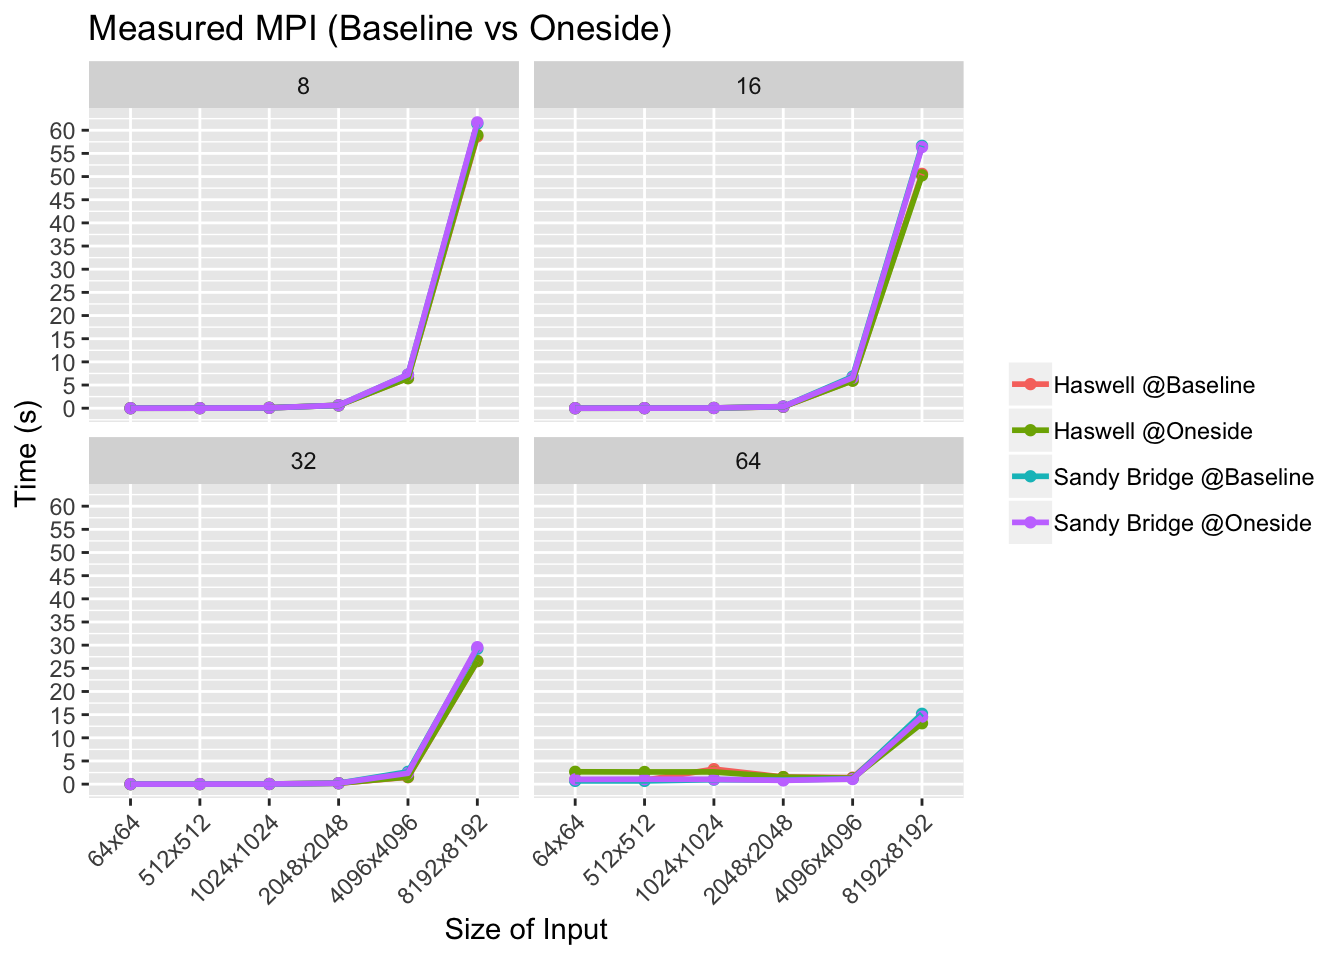
\includegraphics[scale = 0.18]{OSBaseline_Measured-MPI_Processes.png}
%\captionof{figure}{example code for adding pic} 
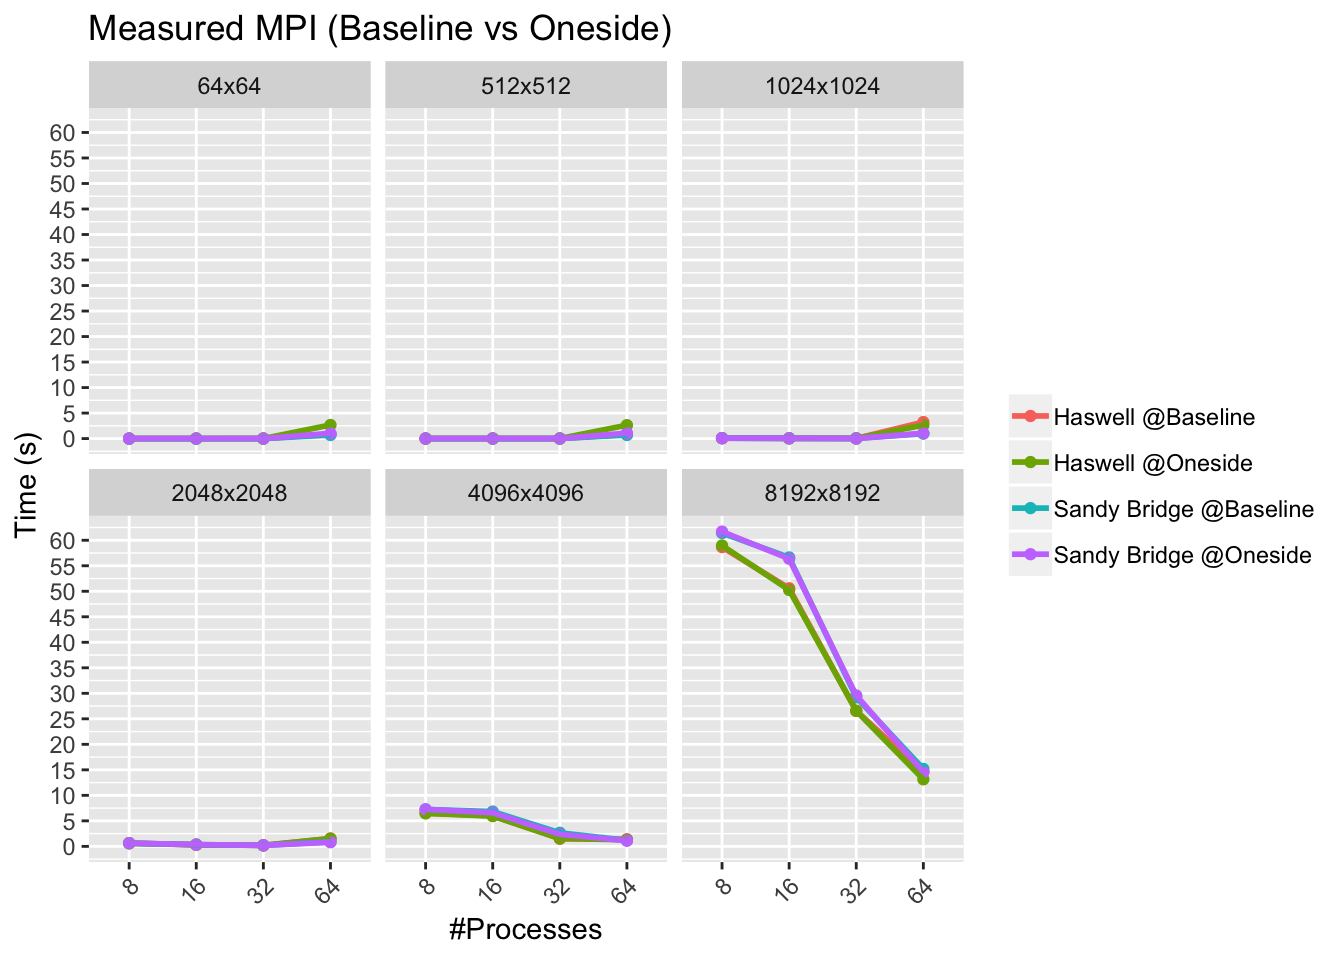
\includegraphics[scale = 0.18]{OSBaseline_Measured-MPI_InputSize.png}
%\captionof{figure}{example code for adding pic} 
\vspace{10mm}
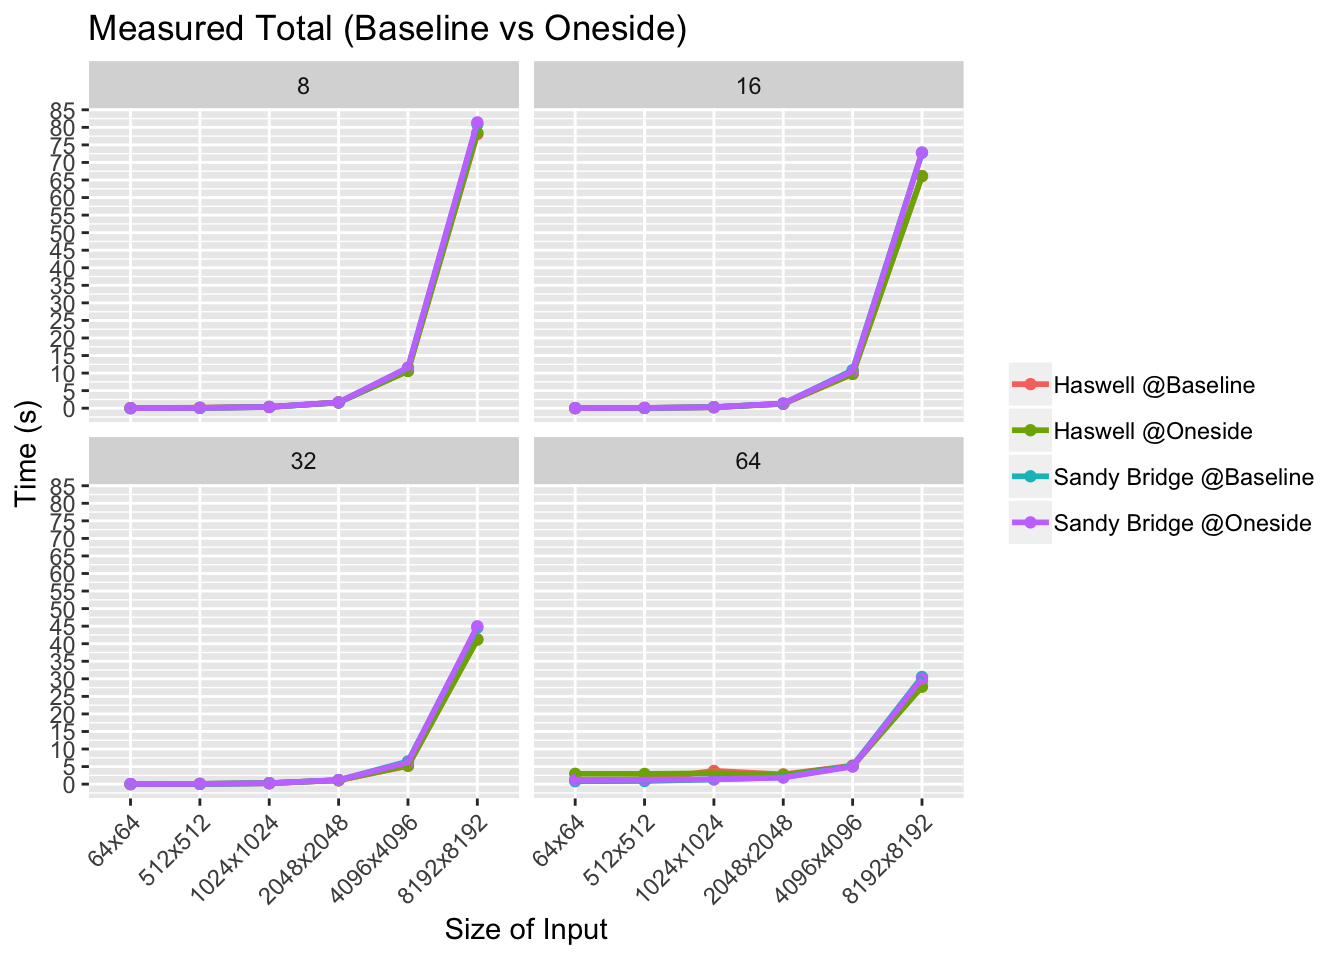
\includegraphics[scale = 0.18]{OSBaseline_Measured-Total_Processes.png}
%\captionof{figure}{example code for adding pic} 
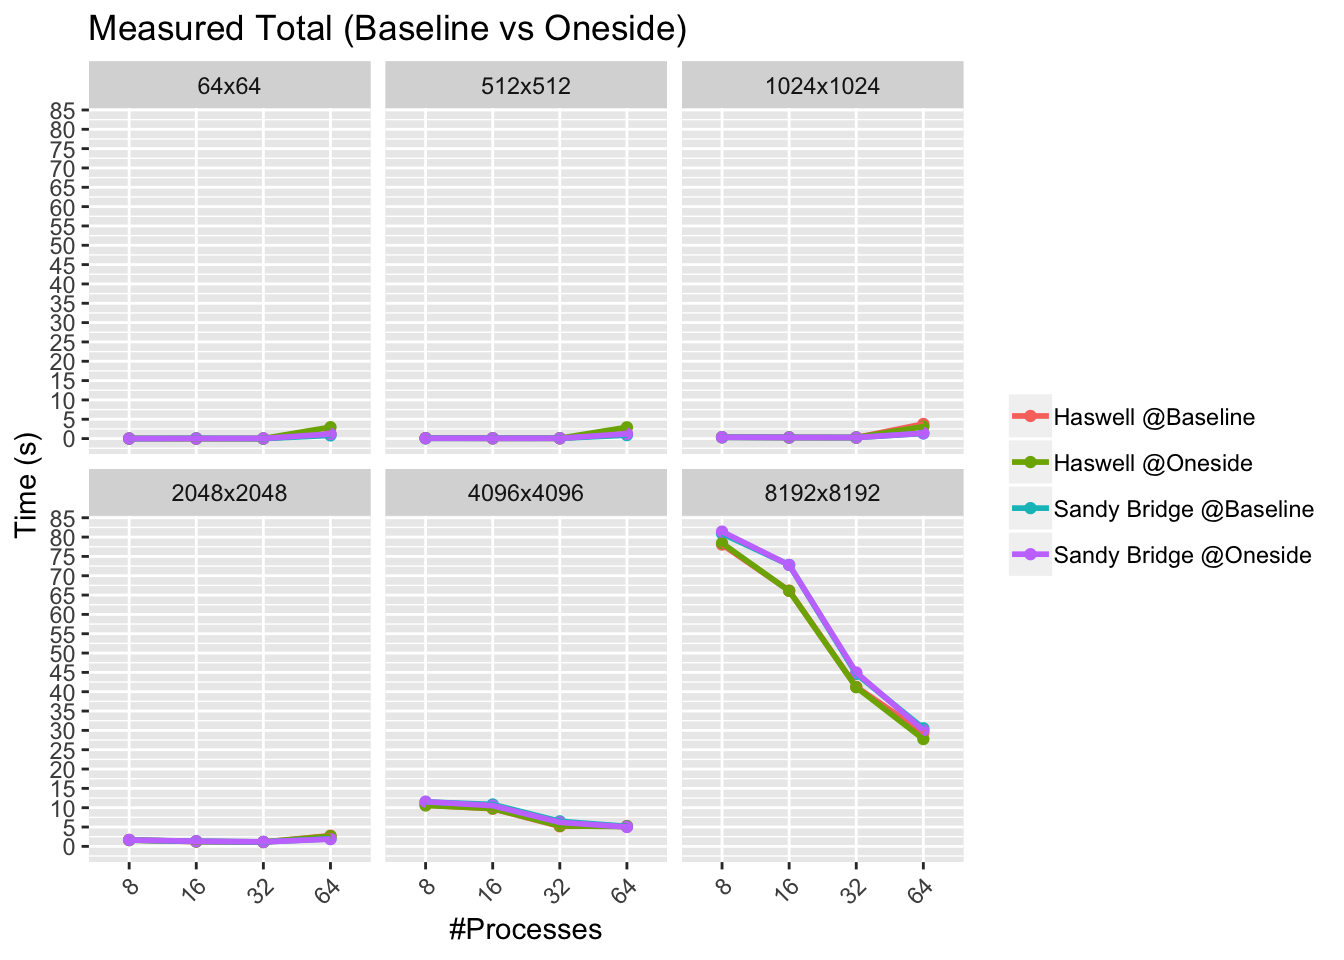
\includegraphics[scale = 0.18]{OSBaseline_Measured-Total_InputSize.png}
%\captionof{figure}{example code for adding pic} 

\item \textbf{Was a speedup observed versus the non-blocking version for the Sandy Bridge and Haswell nodes?} \\

There was little speedup when comparing with the non-blocking version. As we can observe in the plots, the non-blocking communication performed better than the one-sided communication. 

\includegraphics[scale = 0.18]{OSP2P_Measured-Compute_Processes.png}
%\captionof{figure}{example code for adding pic} 
\includegraphics[scale = 0.18]{OSP2P_Measured-Compute_InputSize.png}
%\captionof{figure}{example code for adding pic} 
\vspace{1mm}
\includegraphics[scale = 0.18]{OSP2P_Measured-MPI_Processes.png}
%\captionof{figure}{example code for adding pic} 
\includegraphics[scale = 0.18]{OSP2P_Measured-MPI_InputSize.png}
%\captionof{figure}{example code for adding pic} 
\vspace{1mm}
\includegraphics[scale = 0.18]{OSP2P_Measured-Total_Processes.png}
%\captionof{figure}{example code for adding pic} 
\includegraphics[scale = 0.18]{OSP2P_Measured-Total_InputSize.png}
%\captionof{figure}{example code for adding pic} 
\end{enumerate}

\section{Contribution}

\begin{enumerate}
\item \textbf{Smith} \\ 
 Build and run batch scripts for MPI point-to-point and one-sided communication \\
 Performance analysis with Vampir. \\ 

\item \textbf{Shyam} \\ 
 Understanding of the assignment and final report creation.  \\
 Worked on MPI Point-to-Point Communication\\

\item \textbf{Siddhesh} \\ 
 Worked on MPI One-Sided Communication  \\
\end{enumerate}
\end{titlepage}
\end{document}
